\section{Maxime}

\subsection{Project foundation}
\begin{frame}{Project foundation}
	\begin{center}
	The call center problem 
	\end{center}
\end{frame}

\subsection{Speech}
\begin{frame}{Speech Signal}{Properties}
	\begin{center}
 	\vspace{0.5cm}
	\begin{columns}
		\begin{column}{0.5\textwidth}
		\begin{itemize}		
		\item Voiced Sound
			\begin{itemize}
				\item Periodic 
				\item Low frequencies
			\end{itemize}
		\end{itemize}
		\end{column}
		\begin{column}{0.5\textwidth} 
		\begin{itemize}
		\item Unvoiced Sound 
			\begin{itemize}
				\item Random
				\item High frequencies
			\end{itemize}	
	    \end{itemize}	
		\end{column}
	\end{columns}
	\vspace{1cm}
	We assume the frequency range of speech : 50-4000Hz \\
	Speech can be seen as quasiperiodic and WSS for time frames of 20-30ms 
	\end{center}
\end{frame}

\subsection{Basics of ANC}
\begin{frame}{What Is ANC?}{Introduction}		
	\begin{columns}
		\begin{column}{0.5\textwidth}
				\begin{itemize}
					\item The basic theory of ANC
					\begin{itemize}
						\item  250 Hz
						\item 2500 Hz 
					\end{itemize}	
				\end{itemize}
			\vspace{-2.5mm}	
		\begin{center}
	 		% This file was created by matlab2tikz.
%
%The latest updates can be retrieved from
%  http://www.mathworks.com/matlabcentral/fileexchange/22022-matlab2tikz-matlab2tikz
%where you can also make suggestions and rate matlab2tikz.
%
\definecolor{mycolor1}{rgb}{0.00000,0.44700,0.74100}%
%
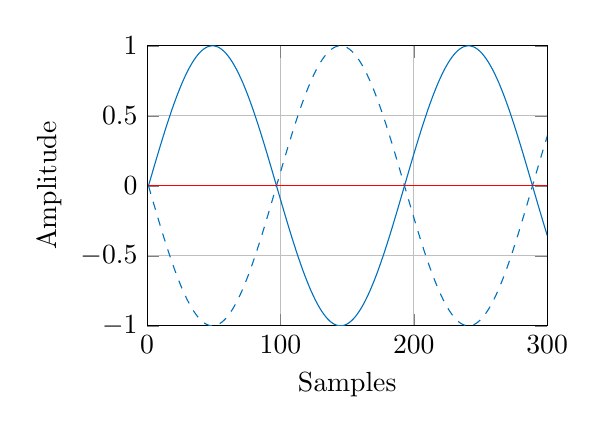
\begin{tikzpicture}

\begin{axis}[%
width=2in,
height=1.4in,
xlabel = {Samples},
ylabel = {Amplitude}, 
scale only axis,
xmin=0,
xmax=300,
xmajorgrids,
ymin=-1,
ymax=1,
ymajorgrids,
axis background/.style={fill=white}
]
\addplot [color=mycolor1,solid,forget plot]
  table[row sep=crcr]{%
1	0\\
2	0.0327190828217761\\
3	0.0654031292301431\\
4	0.0980171403295606\\
5	0.130526192220052\\
6	0.162895473394589\\
7	0.195090322016128\\
8	0.227076263034373\\
9	0.258819045102521\\
10	0.290284677254462\\
11	0.321439465303162\\
12	0.352250047921233\\
13	0.38268343236509\\
14	0.412707029804395\\
15	0.442288690219001\\
16	0.471396736825998\\
17	0.5\\
18	0.528067850650368\\
19	0.555570233019602\\
20	0.582477696867802\\
21	0.608761429008721\\
22	0.634393284163645\\
23	0.659345815100069\\
24	0.683592302022871\\
25	0.707106781186547\\
26	0.729864072697836\\
27	0.751839807478977\\
28	0.773010453362737\\
29	0.793353340291235\\
30	0.812846684591615\\
31	0.831469612302545\\
32	0.849202181526579\\
33	0.866025403784439\\
34	0.881921264348355\\
35	0.896872741532688\\
36	0.910863824921176\\
37	0.923879532511287\\
38	0.935905926757326\\
39	0.946930129495106\\
40	0.956940335732209\\
41	0.965925826289068\\
42	0.973876979277334\\
43	0.98078528040323\\
44	0.986643332084879\\
45	0.99144486137381\\
46	0.995184726672197\\
47	0.997858923238603\\
48	0.999464587476366\\
49	1\\
50	0.999464587476366\\
51	0.997858923238603\\
52	0.995184726672197\\
53	0.99144486137381\\
54	0.986643332084879\\
55	0.980785280403231\\
56	0.973876979277334\\
57	0.965925826289068\\
58	0.956940335732209\\
59	0.946930129495106\\
60	0.935905926757326\\
61	0.923879532511287\\
62	0.910863824921176\\
63	0.896872741532688\\
64	0.881921264348355\\
65	0.866025403784439\\
66	0.849202181526579\\
67	0.831469612302545\\
68	0.812846684591615\\
69	0.793353340291235\\
70	0.773010453362737\\
71	0.751839807478978\\
72	0.729864072697836\\
73	0.707106781186548\\
74	0.683592302022872\\
75	0.659345815100069\\
76	0.634393284163645\\
77	0.60876142900872\\
78	0.582477696867802\\
79	0.555570233019603\\
80	0.528067850650368\\
81	0.5\\
82	0.471396736825998\\
83	0.442288690219002\\
84	0.412707029804395\\
85	0.38268343236509\\
86	0.352250047921233\\
87	0.321439465303161\\
88	0.290284677254463\\
89	0.258819045102521\\
90	0.227076263034374\\
91	0.195090322016129\\
92	0.162895473394589\\
93	0.130526192220052\\
94	0.0980171403295608\\
95	0.0654031292301431\\
96	0.0327190828217764\\
97	1.22464679914735e-16\\
98	-0.0327190828217758\\
99	-0.0654031292301424\\
100	-0.0980171403295606\\
101	-0.130526192220051\\
102	-0.162895473394588\\
103	-0.195090322016128\\
104	-0.227076263034373\\
105	-0.258819045102521\\
106	-0.290284677254462\\
107	-0.321439465303162\\
108	-0.352250047921233\\
109	-0.382683432365089\\
110	-0.412707029804395\\
111	-0.442288690219001\\
112	-0.471396736825998\\
113	-0.5\\
114	-0.528067850650368\\
115	-0.555570233019602\\
116	-0.582477696867802\\
117	-0.608761429008721\\
118	-0.634393284163645\\
119	-0.659345815100069\\
120	-0.683592302022871\\
121	-0.707106781186548\\
122	-0.729864072697836\\
123	-0.751839807478977\\
124	-0.773010453362737\\
125	-0.793353340291235\\
126	-0.812846684591615\\
127	-0.831469612302545\\
128	-0.849202181526579\\
129	-0.866025403784438\\
130	-0.881921264348354\\
131	-0.896872741532688\\
132	-0.910863824921175\\
133	-0.923879532511287\\
134	-0.935905926757326\\
135	-0.946930129495106\\
136	-0.956940335732209\\
137	-0.965925826289068\\
138	-0.973876979277334\\
139	-0.98078528040323\\
140	-0.986643332084879\\
141	-0.99144486137381\\
142	-0.995184726672197\\
143	-0.997858923238603\\
144	-0.999464587476366\\
145	-1\\
146	-0.999464587476366\\
147	-0.997858923238604\\
148	-0.995184726672197\\
149	-0.99144486137381\\
150	-0.986643332084879\\
151	-0.98078528040323\\
152	-0.973876979277334\\
153	-0.965925826289068\\
154	-0.956940335732209\\
155	-0.946930129495105\\
156	-0.935905926757326\\
157	-0.923879532511287\\
158	-0.910863824921176\\
159	-0.896872741532688\\
160	-0.881921264348355\\
161	-0.866025403784439\\
162	-0.849202181526579\\
163	-0.831469612302545\\
164	-0.812846684591615\\
165	-0.793353340291236\\
166	-0.773010453362737\\
167	-0.751839807478978\\
168	-0.729864072697836\\
169	-0.707106781186548\\
170	-0.683592302022872\\
171	-0.659345815100069\\
172	-0.634393284163646\\
173	-0.60876142900872\\
174	-0.582477696867802\\
175	-0.555570233019603\\
176	-0.528067850650368\\
177	-0.5\\
178	-0.471396736825998\\
179	-0.442288690219002\\
180	-0.412707029804395\\
181	-0.38268343236509\\
182	-0.352250047921234\\
183	-0.321439465303162\\
184	-0.290284677254463\\
185	-0.258819045102522\\
186	-0.227076263034374\\
187	-0.195090322016129\\
188	-0.162895473394589\\
189	-0.130526192220052\\
190	-0.0980171403295605\\
191	-0.0654031292301437\\
192	-0.0327190828217766\\
193	-2.44929359829471e-16\\
194	0.0327190828217752\\
195	0.0654031292301423\\
196	0.0980171403295609\\
197	0.13052619222005\\
198	0.162895473394589\\
199	0.195090322016128\\
200	0.227076263034373\\
201	0.25881904510252\\
202	0.290284677254462\\
203	0.321439465303161\\
204	0.352250047921233\\
205	0.382683432365089\\
206	0.412707029804394\\
207	0.442288690219002\\
208	0.471396736825997\\
209	0.5\\
210	0.528067850650368\\
211	0.555570233019601\\
212	0.582477696867802\\
213	0.608761429008721\\
214	0.634393284163645\\
215	0.659345815100068\\
216	0.683592302022872\\
217	0.707106781186547\\
218	0.729864072697836\\
219	0.751839807478978\\
220	0.773010453362736\\
221	0.793353340291235\\
222	0.812846684591615\\
223	0.831469612302545\\
224	0.849202181526578\\
225	0.866025403784438\\
226	0.881921264348355\\
227	0.896872741532689\\
228	0.910863824921175\\
229	0.923879532511287\\
230	0.935905926757326\\
231	0.946930129495105\\
232	0.956940335732209\\
233	0.965925826289068\\
234	0.973876979277334\\
235	0.98078528040323\\
236	0.986643332084879\\
237	0.99144486137381\\
238	0.995184726672197\\
239	0.997858923238603\\
240	0.999464587476366\\
241	1\\
242	0.999464587476366\\
243	0.997858923238603\\
244	0.995184726672197\\
245	0.99144486137381\\
246	0.986643332084879\\
247	0.98078528040323\\
248	0.973876979277334\\
249	0.965925826289068\\
250	0.956940335732209\\
251	0.946930129495106\\
252	0.935905926757325\\
253	0.923879532511287\\
254	0.910863824921176\\
255	0.896872741532688\\
256	0.881921264348355\\
257	0.866025403784439\\
258	0.849202181526579\\
259	0.831469612302547\\
260	0.812846684591615\\
261	0.793353340291235\\
262	0.773010453362738\\
263	0.751839807478978\\
264	0.729864072697835\\
265	0.707106781186548\\
266	0.683592302022871\\
267	0.65934581510007\\
268	0.634393284163647\\
269	0.608761429008721\\
270	0.582477696867803\\
271	0.555570233019602\\
272	0.528067850650369\\
273	0.5\\
274	0.471396736825998\\
275	0.442288690219001\\
276	0.412707029804396\\
277	0.382683432365091\\
278	0.352250047921233\\
279	0.321439465303162\\
280	0.290284677254463\\
281	0.258819045102523\\
282	0.227076263034374\\
283	0.195090322016128\\
284	0.162895473394589\\
285	0.130526192220053\\
286	0.0980171403295624\\
287	0.0654031292301438\\
288	0.0327190828217758\\
289	3.67394039744206e-16\\
290	-0.0327190828217751\\
291	-0.0654031292301431\\
292	-0.0980171403295617\\
293	-0.13052619222005\\
294	-0.162895473394588\\
295	-0.195090322016126\\
296	-0.227076263034373\\
297	-0.25881904510252\\
298	-0.290284677254461\\
299	-0.32143946530316\\
300	-0.352250047921234\\
301	-0.38268343236509\\
302	-0.412707029804394\\
303	-0.442288690219\\
304	-0.471396736825996\\
305	-0.500000000000001\\
306	-0.528067850650368\\
307	-0.555570233019602\\
308	-0.582477696867801\\
309	-0.608761429008722\\
310	-0.634393284163645\\
311	-0.659345815100069\\
312	-0.68359230202287\\
313	-0.707106781186547\\
314	-0.729864072697835\\
315	-0.751839807478977\\
316	-0.773010453362736\\
317	-0.793353340291235\\
318	-0.812846684591614\\
319	-0.831469612302545\\
320	-0.849202181526578\\
321	-0.866025403784438\\
322	-0.881921264348355\\
323	-0.896872741532689\\
324	-0.910863824921176\\
325	-0.923879532511286\\
326	-0.935905926757325\\
327	-0.946930129495105\\
328	-0.956940335732209\\
329	-0.965925826289068\\
330	-0.973876979277333\\
331	-0.98078528040323\\
332	-0.986643332084879\\
333	-0.99144486137381\\
334	-0.995184726672197\\
335	-0.997858923238603\\
336	-0.999464587476366\\
337	-1\\
338	-0.999464587476366\\
339	-0.997858923238604\\
340	-0.995184726672197\\
341	-0.99144486137381\\
342	-0.986643332084879\\
343	-0.980785280403231\\
344	-0.973876979277334\\
345	-0.965925826289068\\
346	-0.956940335732209\\
347	-0.946930129495106\\
348	-0.935905926757326\\
349	-0.923879532511287\\
350	-0.910863824921176\\
351	-0.896872741532688\\
352	-0.881921264348356\\
353	-0.866025403784439\\
354	-0.849202181526579\\
355	-0.831469612302546\\
356	-0.812846684591616\\
357	-0.793353340291236\\
358	-0.773010453362738\\
359	-0.751839807478977\\
360	-0.729864072697836\\
361	-0.707106781186548\\
362	-0.683592302022871\\
363	-0.65934581510007\\
364	-0.634393284163645\\
365	-0.608761429008721\\
366	-0.582477696867803\\
367	-0.555570233019604\\
368	-0.528067850650367\\
369	-0.500000000000001\\
370	-0.471396736825998\\
371	-0.442288690219002\\
372	-0.412707029804395\\
373	-0.382683432365091\\
374	-0.352250047921235\\
375	-0.321439465303162\\
376	-0.290284677254464\\
377	-0.258819045102521\\
378	-0.227076263034376\\
379	-0.195090322016128\\
380	-0.162895473394591\\
381	-0.130526192220053\\
382	-0.0980171403295608\\
383	-0.0654031292301439\\
384	-0.0327190828217795\\
385	-4.89858719658941e-16\\
386	0.032719082821775\\
387	0.0654031292301412\\
388	0.0980171403295598\\
389	0.13052619222005\\
390	0.162895473394588\\
391	0.195090322016129\\
392	0.227076263034373\\
393	0.258819045102518\\
394	0.290284677254461\\
395	0.321439465303161\\
396	0.352250047921232\\
397	0.38268343236509\\
398	0.412707029804394\\
399	0.442288690219\\
400	0.471396736825999\\
401	0.499999999999999\\
402	0.528067850650366\\
403	0.555570233019602\\
404	0.582477696867802\\
405	0.608761429008719\\
406	0.634393284163646\\
407	0.659345815100068\\
408	0.683592302022871\\
409	0.707106781186547\\
410	0.729864072697835\\
411	0.751839807478977\\
412	0.773010453362735\\
413	0.793353340291236\\
414	0.812846684591614\\
415	0.831469612302544\\
416	0.849202181526578\\
417	0.866025403784439\\
418	0.881921264348354\\
419	0.896872741532688\\
420	0.910863824921175\\
421	0.923879532511286\\
422	0.935905926757326\\
423	0.946930129495105\\
424	0.956940335732208\\
425	0.965925826289068\\
426	0.973876979277333\\
427	0.98078528040323\\
428	0.986643332084879\\
429	0.99144486137381\\
430	0.995184726672197\\
431	0.997858923238604\\
432	0.999464587476366\\
433	1\\
434	0.999464587476366\\
435	0.997858923238603\\
436	0.995184726672197\\
437	0.99144486137381\\
438	0.986643332084879\\
439	0.980785280403231\\
440	0.973876979277334\\
441	0.965925826289069\\
442	0.956940335732209\\
443	0.946930129495106\\
444	0.935905926757326\\
445	0.923879532511287\\
446	0.910863824921177\\
447	0.896872741532689\\
448	0.881921264348356\\
449	0.866025403784439\\
450	0.849202181526579\\
451	0.831469612302546\\
452	0.812846684591617\\
453	0.793353340291234\\
454	0.773010453362738\\
455	0.751839807478979\\
456	0.729864072697836\\
457	0.707106781186549\\
458	0.683592302022873\\
459	0.659345815100068\\
460	0.634393284163647\\
461	0.608761429008723\\
462	0.582477696867802\\
463	0.555570233019603\\
464	0.528067850650369\\
465	0.5\\
466	0.471396736825998\\
467	0.442288690219003\\
468	0.412707029804397\\
469	0.382683432365091\\
470	0.352250047921235\\
471	0.321439465303164\\
472	0.290284677254462\\
473	0.258819045102523\\
474	0.227076263034376\\
475	0.19509032201613\\
476	0.162895473394589\\
477	0.130526192220053\\
478	0.0980171403295609\\
479	0.0654031292301458\\
480	0.0327190828217761\\
481	-1.16403343982657e-15\\
482	-0.0327190828217784\\
483	-0.0654031292301428\\
484	-0.0980171403295579\\
485	-0.130526192220055\\
486	-0.16289547339459\\
487	-0.195090322016127\\
488	-0.227076263034373\\
489	-0.258819045102523\\
490	-0.290284677254461\\
491	-0.321439465303161\\
492	-0.352250047921237\\
493	-0.382683432365091\\
494	-0.412707029804397\\
495	-0.442288690219001\\
496	-0.471396736825999\\
497	-0.499999999999999\\
498	-0.528067850650368\\
499	-0.5555702330196\\
500	-0.582477696867804\\
501	-0.608761429008723\\
502	-0.634393284163646\\
503	-0.65934581510007\\
504	-0.683592302022873\\
505	-0.707106781186548\\
506	-0.729864072697834\\
507	-0.751839807478977\\
508	-0.773010453362737\\
509	-0.793353340291236\\
510	-0.812846684591616\\
511	-0.831469612302547\\
512	-0.849202181526579\\
513	-0.866025403784439\\
514	-0.881921264348355\\
515	-0.896872741532688\\
516	-0.910863824921176\\
517	-0.923879532511286\\
518	-0.935905926757326\\
519	-0.946930129495107\\
520	-0.956940335732209\\
521	-0.965925826289068\\
522	-0.973876979277334\\
523	-0.980785280403231\\
524	-0.986643332084879\\
525	-0.99144486137381\\
526	-0.995184726672197\\
527	-0.997858923238604\\
528	-0.999464587476366\\
529	-1\\
530	-0.999464587476366\\
531	-0.997858923238603\\
532	-0.995184726672197\\
533	-0.991444861373811\\
534	-0.986643332084879\\
535	-0.98078528040323\\
536	-0.973876979277333\\
537	-0.965925826289069\\
538	-0.956940335732208\\
539	-0.946930129495105\\
540	-0.935905926757326\\
541	-0.923879532511287\\
542	-0.910863824921175\\
543	-0.896872741532689\\
544	-0.881921264348355\\
545	-0.866025403784438\\
546	-0.849202181526578\\
547	-0.831469612302544\\
548	-0.812846684591615\\
549	-0.793353340291234\\
550	-0.773010453362736\\
551	-0.751839807478978\\
552	-0.729864072697837\\
553	-0.707106781186546\\
554	-0.683592302022869\\
555	-0.659345815100069\\
556	-0.634393284163644\\
557	-0.608761429008719\\
558	-0.582477696867802\\
559	-0.555570233019604\\
560	-0.528067850650369\\
561	-0.5\\
562	-0.471396736826\\
563	-0.442288690218999\\
564	-0.412707029804392\\
565	-0.382683432365089\\
566	-0.352250047921232\\
567	-0.321439465303162\\
568	-0.290284677254462\\
569	-0.258819045102519\\
570	-0.227076263034374\\
571	-0.195090322016132\\
572	-0.162895473394588\\
573	-0.13052619222005\\
574	-0.098017140329561\\
575	-0.0654031292301424\\
576	-0.0327190828217744\\
577	-7.34788079488412e-16\\
578	0.0327190828217765\\
579	0.0654031292301409\\
580	0.0980171403295595\\
581	0.130526192220055\\
582	0.16289547339459\\
583	0.19509032201613\\
584	0.227076263034376\\
585	0.258819045102521\\
586	0.290284677254461\\
587	0.321439465303164\\
588	0.352250047921234\\
589	0.382683432365088\\
590	0.412707029804397\\
591	0.442288690219005\\
592	0.471396736825999\\
593	0.500000000000002\\
594	0.528067850650368\\
595	0.555570233019603\\
596	0.582477696867804\\
597	0.608761429008717\\
598	0.634393284163646\\
599	0.65934581510007\\
600	0.683592302022871\\
601	0.707106781186548\\
602	0.729864072697836\\
603	0.751839807478977\\
604	0.773010453362737\\
605	0.793353340291236\\
606	0.812846684591614\\
607	0.831469612302545\\
608	0.849202181526579\\
609	0.866025403784439\\
610	0.881921264348356\\
611	0.896872741532688\\
612	0.910863824921175\\
613	0.923879532511286\\
614	0.935905926757326\\
615	0.946930129495105\\
616	0.956940335732208\\
617	0.965925826289069\\
618	0.973876979277334\\
619	0.980785280403231\\
620	0.986643332084879\\
621	0.99144486137381\\
622	0.995184726672197\\
623	0.997858923238603\\
624	0.999464587476366\\
625	1\\
626	0.999464587476366\\
627	0.997858923238604\\
628	0.995184726672197\\
629	0.99144486137381\\
630	0.986643332084879\\
631	0.98078528040323\\
632	0.973876979277334\\
633	0.965925826289069\\
634	0.956940335732209\\
635	0.946930129495105\\
636	0.935905926757325\\
637	0.923879532511286\\
638	0.910863824921176\\
639	0.896872741532689\\
640	0.881921264348354\\
641	0.866025403784438\\
642	0.84920218152658\\
643	0.831469612302546\\
644	0.812846684591613\\
645	0.793353340291235\\
646	0.773010453362736\\
647	0.751839807478978\\
648	0.729864072697835\\
649	0.707106781186546\\
650	0.683592302022872\\
651	0.659345815100069\\
652	0.634393284163644\\
653	0.608761429008721\\
654	0.582477696867802\\
655	0.555570233019601\\
656	0.528067850650369\\
657	0.5\\
658	0.471396736825997\\
659	0.442288690219003\\
660	0.412707029804395\\
661	0.382683432365089\\
662	0.352250047921232\\
663	0.321439465303159\\
664	0.290284677254459\\
665	0.258819045102523\\
666	0.227076263034374\\
667	0.195090322016125\\
668	0.162895473394591\\
669	0.130526192220053\\
670	0.0980171403295611\\
671	0.0654031292301425\\
672	0.0327190828217745\\
673	8.57252759403147e-16\\
674	-0.0327190828217764\\
675	-0.0654031292301444\\
676	-0.0980171403295594\\
677	-0.130526192220048\\
678	-0.16289547339459\\
679	-0.195090322016127\\
680	-0.227076263034373\\
681	-0.258819045102521\\
682	-0.290284677254464\\
683	-0.321439465303161\\
684	-0.352250047921234\\
685	-0.382683432365091\\
686	-0.412707029804394\\
687	-0.442288690219001\\
688	-0.471396736825995\\
689	-0.500000000000002\\
690	-0.528067850650371\\
691	-0.555570233019603\\
692	-0.582477696867801\\
693	-0.608761429008723\\
694	-0.634393284163646\\
695	-0.659345815100067\\
696	-0.68359230202287\\
697	-0.707106781186548\\
698	-0.729864072697836\\
699	-0.751839807478979\\
700	-0.773010453362737\\
701	-0.793353340291236\\
702	-0.812846684591616\\
703	-0.831469612302545\\
704	-0.849202181526579\\
705	-0.866025403784439\\
706	-0.881921264348355\\
707	-0.896872741532688\\
708	-0.910863824921176\\
709	-0.923879532511288\\
710	-0.935905926757326\\
711	-0.946930129495106\\
712	-0.956940335732209\\
713	-0.965925826289068\\
714	-0.973876979277334\\
715	-0.98078528040323\\
716	-0.986643332084879\\
717	-0.991444861373811\\
718	-0.995184726672197\\
719	-0.997858923238603\\
720	-0.999464587476366\\
721	-1\\
722	-0.999464587476366\\
723	-0.997858923238604\\
724	-0.995184726672197\\
725	-0.99144486137381\\
726	-0.986643332084879\\
727	-0.98078528040323\\
728	-0.973876979277333\\
729	-0.965925826289069\\
730	-0.956940335732209\\
731	-0.946930129495105\\
732	-0.935905926757326\\
733	-0.923879532511288\\
734	-0.910863824921176\\
735	-0.896872741532688\\
736	-0.881921264348355\\
737	-0.866025403784438\\
738	-0.849202181526578\\
739	-0.831469612302546\\
740	-0.812846684591615\\
741	-0.793353340291237\\
742	-0.773010453362738\\
743	-0.751839807478975\\
744	-0.729864072697835\\
745	-0.707106781186549\\
746	-0.683592302022869\\
747	-0.659345815100069\\
748	-0.634393284163647\\
749	-0.608761429008722\\
750	-0.582477696867802\\
751	-0.555570233019604\\
752	-0.528067850650366\\
753	-0.499999999999997\\
754	-0.471396736825997\\
755	-0.442288690219\\
756	-0.412707029804392\\
757	-0.382683432365089\\
758	-0.352250047921232\\
759	-0.321439465303159\\
760	-0.290284677254466\\
761	-0.25881904510252\\
762	-0.227076263034368\\
763	-0.195090322016129\\
764	-0.162895473394588\\
765	-0.13052619222005\\
766	-0.0980171403295612\\
767	-0.0654031292301426\\
768	-0.0327190828217746\\
769	-9.79717439317883e-16\\
770	0.0327190828217798\\
771	0.0654031292301478\\
772	0.0980171403295593\\
773	0.130526192220055\\
774	0.162895473394586\\
775	0.195090322016127\\
776	0.227076263034373\\
777	0.258819045102518\\
778	0.29028467725446\\
779	0.321439465303164\\
780	0.352250047921234\\
781	0.382683432365091\\
782	0.412707029804397\\
783	0.442288690219001\\
784	0.471396736825998\\
785	0.500000000000002\\
786	0.528067850650365\\
787	0.5555702330196\\
788	0.582477696867806\\
789	0.60876142900872\\
790	0.634393284163646\\
791	0.65934581510007\\
792	0.68359230202287\\
793	0.707106781186547\\
794	0.729864072697836\\
795	0.751839807478976\\
796	0.773010453362737\\
797	0.793353340291238\\
798	0.812846684591614\\
799	0.831469612302547\\
800	0.849202181526577\\
801	0.866025403784437\\
802	0.881921264348354\\
803	0.896872741532687\\
804	0.910863824921175\\
805	0.923879532511286\\
806	0.935905926757326\\
807	0.946930129495106\\
808	0.956940335732209\\
809	0.965925826289067\\
810	0.973876979277334\\
811	0.980785280403231\\
812	0.986643332084878\\
813	0.99144486137381\\
814	0.995184726672197\\
815	0.997858923238603\\
816	0.999464587476366\\
817	1\\
818	0.999464587476366\\
819	0.997858923238604\\
820	0.995184726672197\\
821	0.991444861373811\\
822	0.986643332084879\\
823	0.98078528040323\\
824	0.973876979277334\\
825	0.965925826289068\\
826	0.956940335732208\\
827	0.946930129495107\\
828	0.935905926757326\\
829	0.923879532511287\\
830	0.910863824921177\\
831	0.896872741532689\\
832	0.881921264348355\\
833	0.866025403784439\\
834	0.849202181526578\\
835	0.831469612302544\\
836	0.812846684591615\\
837	0.793353340291235\\
838	0.773010453362736\\
839	0.75183980747898\\
840	0.729864072697838\\
841	0.707106781186546\\
842	0.683592302022872\\
843	0.659345815100069\\
844	0.634393284163644\\
845	0.608761429008722\\
846	0.582477696867802\\
847	0.555570233019602\\
848	0.528067850650369\\
849	0.5\\
850	0.471396736825997\\
851	0.442288690219003\\
852	0.412707029804392\\
853	0.382683432365086\\
854	0.352250047921236\\
855	0.321439465303163\\
856	0.290284677254462\\
857	0.258819045102523\\
858	0.227076263034375\\
859	0.195090322016129\\
860	0.162895473394588\\
861	0.13052619222005\\
862	0.0980171403295578\\
863	0.0654031292301428\\
864	0.0327190828217748\\
865	-2.45053155956788e-15\\
866	-0.0327190828217726\\
867	-0.0654031292301441\\
868	-0.0980171403295627\\
869	-0.130526192220051\\
870	-0.162895473394589\\
871	-0.19509032201613\\
872	-0.227076263034373\\
873	-0.258819045102521\\
874	-0.290284677254464\\
875	-0.321439465303161\\
876	-0.352250047921234\\
877	-0.382683432365084\\
878	-0.412707029804397\\
879	-0.442288690219004\\
880	-0.471396736825995\\
881	-0.499999999999999\\
882	-0.528067850650367\\
883	-0.5555702330196\\
884	-0.5824776968678\\
885	-0.60876142900872\\
886	-0.634393284163643\\
887	-0.65934581510007\\
888	-0.683592302022873\\
889	-0.707106781186547\\
890	-0.729864072697836\\
891	-0.751839807478979\\
892	-0.773010453362734\\
893	-0.793353340291233\\
894	-0.812846684591616\\
895	-0.831469612302543\\
896	-0.849202181526579\\
897	-0.866025403784439\\
898	-0.881921264348354\\
899	-0.896872741532688\\
900	-0.910863824921176\\
901	-0.923879532511286\\
902	-0.935905926757326\\
903	-0.946930129495106\\
904	-0.956940335732207\\
905	-0.965925826289069\\
906	-0.973876979277335\\
907	-0.98078528040323\\
908	-0.986643332084879\\
909	-0.99144486137381\\
910	-0.995184726672197\\
911	-0.997858923238603\\
912	-0.999464587476366\\
913	-1\\
914	-0.999464587476366\\
915	-0.997858923238603\\
916	-0.995184726672197\\
917	-0.99144486137381\\
918	-0.986643332084879\\
919	-0.980785280403231\\
920	-0.973876979277333\\
921	-0.965925826289068\\
922	-0.95694033573221\\
923	-0.946930129495105\\
924	-0.935905926757325\\
925	-0.923879532511287\\
926	-0.910863824921176\\
927	-0.896872741532688\\
928	-0.881921264348355\\
929	-0.866025403784439\\
930	-0.849202181526582\\
931	-0.831469612302546\\
932	-0.812846684591613\\
933	-0.793353340291237\\
934	-0.773010453362738\\
935	-0.751839807478978\\
936	-0.729864072697838\\
937	-0.707106781186549\\
938	-0.683592302022872\\
939	-0.659345815100072\\
940	-0.634393284163647\\
941	-0.608761429008719\\
942	-0.582477696867802\\
943	-0.555570233019602\\
944	-0.528067850650366\\
945	-0.500000000000004\\
946	-0.471396736826\\
947	-0.442288690219\\
948	-0.412707029804399\\
949	-0.382683432365093\\
950	-0.352250047921232\\
951	-0.321439465303163\\
952	-0.290284677254463\\
953	-0.25881904510252\\
954	-0.227076263034375\\
955	-0.195090322016129\\
956	-0.162895473394592\\
957	-0.130526192220057\\
958	-0.0980171403295615\\
959	-0.0654031292301429\\
960	-0.0327190828217784\\
961	2.32806687965315e-15\\
};
\addplot [color=mycolor1,dashed,forget plot]
  table[row sep=crcr]{%
1	-0\\
2	-0.0327190828217761\\
3	-0.0654031292301431\\
4	-0.0980171403295606\\
5	-0.130526192220052\\
6	-0.162895473394589\\
7	-0.195090322016128\\
8	-0.227076263034373\\
9	-0.258819045102521\\
10	-0.290284677254462\\
11	-0.321439465303162\\
12	-0.352250047921233\\
13	-0.38268343236509\\
14	-0.412707029804395\\
15	-0.442288690219001\\
16	-0.471396736825998\\
17	-0.5\\
18	-0.528067850650368\\
19	-0.555570233019602\\
20	-0.582477696867802\\
21	-0.608761429008721\\
22	-0.634393284163645\\
23	-0.659345815100069\\
24	-0.683592302022871\\
25	-0.707106781186547\\
26	-0.729864072697836\\
27	-0.751839807478977\\
28	-0.773010453362737\\
29	-0.793353340291235\\
30	-0.812846684591615\\
31	-0.831469612302545\\
32	-0.849202181526579\\
33	-0.866025403784439\\
34	-0.881921264348355\\
35	-0.896872741532688\\
36	-0.910863824921176\\
37	-0.923879532511287\\
38	-0.935905926757326\\
39	-0.946930129495106\\
40	-0.956940335732209\\
41	-0.965925826289068\\
42	-0.973876979277334\\
43	-0.98078528040323\\
44	-0.986643332084879\\
45	-0.99144486137381\\
46	-0.995184726672197\\
47	-0.997858923238603\\
48	-0.999464587476366\\
49	-1\\
50	-0.999464587476366\\
51	-0.997858923238603\\
52	-0.995184726672197\\
53	-0.99144486137381\\
54	-0.986643332084879\\
55	-0.980785280403231\\
56	-0.973876979277334\\
57	-0.965925826289068\\
58	-0.956940335732209\\
59	-0.946930129495106\\
60	-0.935905926757326\\
61	-0.923879532511287\\
62	-0.910863824921176\\
63	-0.896872741532688\\
64	-0.881921264348355\\
65	-0.866025403784439\\
66	-0.849202181526579\\
67	-0.831469612302545\\
68	-0.812846684591615\\
69	-0.793353340291235\\
70	-0.773010453362737\\
71	-0.751839807478978\\
72	-0.729864072697836\\
73	-0.707106781186548\\
74	-0.683592302022872\\
75	-0.659345815100069\\
76	-0.634393284163645\\
77	-0.60876142900872\\
78	-0.582477696867802\\
79	-0.555570233019603\\
80	-0.528067850650368\\
81	-0.5\\
82	-0.471396736825998\\
83	-0.442288690219002\\
84	-0.412707029804395\\
85	-0.38268343236509\\
86	-0.352250047921233\\
87	-0.321439465303161\\
88	-0.290284677254463\\
89	-0.258819045102521\\
90	-0.227076263034374\\
91	-0.195090322016129\\
92	-0.162895473394589\\
93	-0.130526192220052\\
94	-0.0980171403295608\\
95	-0.0654031292301431\\
96	-0.0327190828217764\\
97	-1.22464679914735e-16\\
98	0.0327190828217758\\
99	0.0654031292301424\\
100	0.0980171403295606\\
101	0.130526192220051\\
102	0.162895473394588\\
103	0.195090322016128\\
104	0.227076263034373\\
105	0.258819045102521\\
106	0.290284677254462\\
107	0.321439465303162\\
108	0.352250047921233\\
109	0.382683432365089\\
110	0.412707029804395\\
111	0.442288690219001\\
112	0.471396736825998\\
113	0.5\\
114	0.528067850650368\\
115	0.555570233019602\\
116	0.582477696867802\\
117	0.608761429008721\\
118	0.634393284163645\\
119	0.659345815100069\\
120	0.683592302022871\\
121	0.707106781186548\\
122	0.729864072697836\\
123	0.751839807478977\\
124	0.773010453362737\\
125	0.793353340291235\\
126	0.812846684591615\\
127	0.831469612302545\\
128	0.849202181526579\\
129	0.866025403784438\\
130	0.881921264348354\\
131	0.896872741532688\\
132	0.910863824921175\\
133	0.923879532511287\\
134	0.935905926757326\\
135	0.946930129495106\\
136	0.956940335732209\\
137	0.965925826289068\\
138	0.973876979277334\\
139	0.98078528040323\\
140	0.986643332084879\\
141	0.99144486137381\\
142	0.995184726672197\\
143	0.997858923238603\\
144	0.999464587476366\\
145	1\\
146	0.999464587476366\\
147	0.997858923238604\\
148	0.995184726672197\\
149	0.99144486137381\\
150	0.986643332084879\\
151	0.98078528040323\\
152	0.973876979277334\\
153	0.965925826289068\\
154	0.956940335732209\\
155	0.946930129495105\\
156	0.935905926757326\\
157	0.923879532511287\\
158	0.910863824921176\\
159	0.896872741532688\\
160	0.881921264348355\\
161	0.866025403784439\\
162	0.849202181526579\\
163	0.831469612302545\\
164	0.812846684591615\\
165	0.793353340291236\\
166	0.773010453362737\\
167	0.751839807478978\\
168	0.729864072697836\\
169	0.707106781186548\\
170	0.683592302022872\\
171	0.659345815100069\\
172	0.634393284163646\\
173	0.60876142900872\\
174	0.582477696867802\\
175	0.555570233019603\\
176	0.528067850650368\\
177	0.5\\
178	0.471396736825998\\
179	0.442288690219002\\
180	0.412707029804395\\
181	0.38268343236509\\
182	0.352250047921234\\
183	0.321439465303162\\
184	0.290284677254463\\
185	0.258819045102522\\
186	0.227076263034374\\
187	0.195090322016129\\
188	0.162895473394589\\
189	0.130526192220052\\
190	0.0980171403295605\\
191	0.0654031292301437\\
192	0.0327190828217766\\
193	2.44929359829471e-16\\
194	-0.0327190828217752\\
195	-0.0654031292301423\\
196	-0.0980171403295609\\
197	-0.13052619222005\\
198	-0.162895473394589\\
199	-0.195090322016128\\
200	-0.227076263034373\\
201	-0.25881904510252\\
202	-0.290284677254462\\
203	-0.321439465303161\\
204	-0.352250047921233\\
205	-0.382683432365089\\
206	-0.412707029804394\\
207	-0.442288690219002\\
208	-0.471396736825997\\
209	-0.5\\
210	-0.528067850650368\\
211	-0.555570233019601\\
212	-0.582477696867802\\
213	-0.608761429008721\\
214	-0.634393284163645\\
215	-0.659345815100068\\
216	-0.683592302022872\\
217	-0.707106781186547\\
218	-0.729864072697836\\
219	-0.751839807478978\\
220	-0.773010453362736\\
221	-0.793353340291235\\
222	-0.812846684591615\\
223	-0.831469612302545\\
224	-0.849202181526578\\
225	-0.866025403784438\\
226	-0.881921264348355\\
227	-0.896872741532689\\
228	-0.910863824921175\\
229	-0.923879532511287\\
230	-0.935905926757326\\
231	-0.946930129495105\\
232	-0.956940335732209\\
233	-0.965925826289068\\
234	-0.973876979277334\\
235	-0.98078528040323\\
236	-0.986643332084879\\
237	-0.99144486137381\\
238	-0.995184726672197\\
239	-0.997858923238603\\
240	-0.999464587476366\\
241	-1\\
242	-0.999464587476366\\
243	-0.997858923238603\\
244	-0.995184726672197\\
245	-0.99144486137381\\
246	-0.986643332084879\\
247	-0.98078528040323\\
248	-0.973876979277334\\
249	-0.965925826289068\\
250	-0.956940335732209\\
251	-0.946930129495106\\
252	-0.935905926757325\\
253	-0.923879532511287\\
254	-0.910863824921176\\
255	-0.896872741532688\\
256	-0.881921264348355\\
257	-0.866025403784439\\
258	-0.849202181526579\\
259	-0.831469612302547\\
260	-0.812846684591615\\
261	-0.793353340291235\\
262	-0.773010453362738\\
263	-0.751839807478978\\
264	-0.729864072697835\\
265	-0.707106781186548\\
266	-0.683592302022871\\
267	-0.65934581510007\\
268	-0.634393284163647\\
269	-0.608761429008721\\
270	-0.582477696867803\\
271	-0.555570233019602\\
272	-0.528067850650369\\
273	-0.5\\
274	-0.471396736825998\\
275	-0.442288690219001\\
276	-0.412707029804396\\
277	-0.382683432365091\\
278	-0.352250047921233\\
279	-0.321439465303162\\
280	-0.290284677254463\\
281	-0.258819045102523\\
282	-0.227076263034374\\
283	-0.195090322016128\\
284	-0.162895473394589\\
285	-0.130526192220053\\
286	-0.0980171403295624\\
287	-0.0654031292301438\\
288	-0.0327190828217758\\
289	-3.67394039744206e-16\\
290	0.0327190828217751\\
291	0.0654031292301431\\
292	0.0980171403295617\\
293	0.13052619222005\\
294	0.162895473394588\\
295	0.195090322016126\\
296	0.227076263034373\\
297	0.25881904510252\\
298	0.290284677254461\\
299	0.32143946530316\\
300	0.352250047921234\\
301	0.38268343236509\\
302	0.412707029804394\\
303	0.442288690219\\
304	0.471396736825996\\
305	0.500000000000001\\
306	0.528067850650368\\
307	0.555570233019602\\
308	0.582477696867801\\
309	0.608761429008722\\
310	0.634393284163645\\
311	0.659345815100069\\
312	0.68359230202287\\
313	0.707106781186547\\
314	0.729864072697835\\
315	0.751839807478977\\
316	0.773010453362736\\
317	0.793353340291235\\
318	0.812846684591614\\
319	0.831469612302545\\
320	0.849202181526578\\
321	0.866025403784438\\
322	0.881921264348355\\
323	0.896872741532689\\
324	0.910863824921176\\
325	0.923879532511286\\
326	0.935905926757325\\
327	0.946930129495105\\
328	0.956940335732209\\
329	0.965925826289068\\
330	0.973876979277333\\
331	0.98078528040323\\
332	0.986643332084879\\
333	0.99144486137381\\
334	0.995184726672197\\
335	0.997858923238603\\
336	0.999464587476366\\
337	1\\
338	0.999464587476366\\
339	0.997858923238604\\
340	0.995184726672197\\
341	0.99144486137381\\
342	0.986643332084879\\
343	0.980785280403231\\
344	0.973876979277334\\
345	0.965925826289068\\
346	0.956940335732209\\
347	0.946930129495106\\
348	0.935905926757326\\
349	0.923879532511287\\
350	0.910863824921176\\
351	0.896872741532688\\
352	0.881921264348356\\
353	0.866025403784439\\
354	0.849202181526579\\
355	0.831469612302546\\
356	0.812846684591616\\
357	0.793353340291236\\
358	0.773010453362738\\
359	0.751839807478977\\
360	0.729864072697836\\
361	0.707106781186548\\
362	0.683592302022871\\
363	0.65934581510007\\
364	0.634393284163645\\
365	0.608761429008721\\
366	0.582477696867803\\
367	0.555570233019604\\
368	0.528067850650367\\
369	0.500000000000001\\
370	0.471396736825998\\
371	0.442288690219002\\
372	0.412707029804395\\
373	0.382683432365091\\
374	0.352250047921235\\
375	0.321439465303162\\
376	0.290284677254464\\
377	0.258819045102521\\
378	0.227076263034376\\
379	0.195090322016128\\
380	0.162895473394591\\
381	0.130526192220053\\
382	0.0980171403295608\\
383	0.0654031292301439\\
384	0.0327190828217795\\
385	4.89858719658941e-16\\
386	-0.032719082821775\\
387	-0.0654031292301412\\
388	-0.0980171403295598\\
389	-0.13052619222005\\
390	-0.162895473394588\\
391	-0.195090322016129\\
392	-0.227076263034373\\
393	-0.258819045102518\\
394	-0.290284677254461\\
395	-0.321439465303161\\
396	-0.352250047921232\\
397	-0.38268343236509\\
398	-0.412707029804394\\
399	-0.442288690219\\
400	-0.471396736825999\\
401	-0.499999999999999\\
402	-0.528067850650366\\
403	-0.555570233019602\\
404	-0.582477696867802\\
405	-0.608761429008719\\
406	-0.634393284163646\\
407	-0.659345815100068\\
408	-0.683592302022871\\
409	-0.707106781186547\\
410	-0.729864072697835\\
411	-0.751839807478977\\
412	-0.773010453362735\\
413	-0.793353340291236\\
414	-0.812846684591614\\
415	-0.831469612302544\\
416	-0.849202181526578\\
417	-0.866025403784439\\
418	-0.881921264348354\\
419	-0.896872741532688\\
420	-0.910863824921175\\
421	-0.923879532511286\\
422	-0.935905926757326\\
423	-0.946930129495105\\
424	-0.956940335732208\\
425	-0.965925826289068\\
426	-0.973876979277333\\
427	-0.98078528040323\\
428	-0.986643332084879\\
429	-0.99144486137381\\
430	-0.995184726672197\\
431	-0.997858923238604\\
432	-0.999464587476366\\
433	-1\\
434	-0.999464587476366\\
435	-0.997858923238603\\
436	-0.995184726672197\\
437	-0.99144486137381\\
438	-0.986643332084879\\
439	-0.980785280403231\\
440	-0.973876979277334\\
441	-0.965925826289069\\
442	-0.956940335732209\\
443	-0.946930129495106\\
444	-0.935905926757326\\
445	-0.923879532511287\\
446	-0.910863824921177\\
447	-0.896872741532689\\
448	-0.881921264348356\\
449	-0.866025403784439\\
450	-0.849202181526579\\
451	-0.831469612302546\\
452	-0.812846684591617\\
453	-0.793353340291234\\
454	-0.773010453362738\\
455	-0.751839807478979\\
456	-0.729864072697836\\
457	-0.707106781186549\\
458	-0.683592302022873\\
459	-0.659345815100068\\
460	-0.634393284163647\\
461	-0.608761429008723\\
462	-0.582477696867802\\
463	-0.555570233019603\\
464	-0.528067850650369\\
465	-0.5\\
466	-0.471396736825998\\
467	-0.442288690219003\\
468	-0.412707029804397\\
469	-0.382683432365091\\
470	-0.352250047921235\\
471	-0.321439465303164\\
472	-0.290284677254462\\
473	-0.258819045102523\\
474	-0.227076263034376\\
475	-0.19509032201613\\
476	-0.162895473394589\\
477	-0.130526192220053\\
478	-0.0980171403295609\\
479	-0.0654031292301458\\
480	-0.0327190828217761\\
481	1.16403343982657e-15\\
482	0.0327190828217784\\
483	0.0654031292301428\\
484	0.0980171403295579\\
485	0.130526192220055\\
486	0.16289547339459\\
487	0.195090322016127\\
488	0.227076263034373\\
489	0.258819045102523\\
490	0.290284677254461\\
491	0.321439465303161\\
492	0.352250047921237\\
493	0.382683432365091\\
494	0.412707029804397\\
495	0.442288690219001\\
496	0.471396736825999\\
497	0.499999999999999\\
498	0.528067850650368\\
499	0.5555702330196\\
500	0.582477696867804\\
501	0.608761429008723\\
502	0.634393284163646\\
503	0.65934581510007\\
504	0.683592302022873\\
505	0.707106781186548\\
506	0.729864072697834\\
507	0.751839807478977\\
508	0.773010453362737\\
509	0.793353340291236\\
510	0.812846684591616\\
511	0.831469612302547\\
512	0.849202181526579\\
513	0.866025403784439\\
514	0.881921264348355\\
515	0.896872741532688\\
516	0.910863824921176\\
517	0.923879532511286\\
518	0.935905926757326\\
519	0.946930129495107\\
520	0.956940335732209\\
521	0.965925826289068\\
522	0.973876979277334\\
523	0.980785280403231\\
524	0.986643332084879\\
525	0.99144486137381\\
526	0.995184726672197\\
527	0.997858923238604\\
528	0.999464587476366\\
529	1\\
530	0.999464587476366\\
531	0.997858923238603\\
532	0.995184726672197\\
533	0.991444861373811\\
534	0.986643332084879\\
535	0.98078528040323\\
536	0.973876979277333\\
537	0.965925826289069\\
538	0.956940335732208\\
539	0.946930129495105\\
540	0.935905926757326\\
541	0.923879532511287\\
542	0.910863824921175\\
543	0.896872741532689\\
544	0.881921264348355\\
545	0.866025403784438\\
546	0.849202181526578\\
547	0.831469612302544\\
548	0.812846684591615\\
549	0.793353340291234\\
550	0.773010453362736\\
551	0.751839807478978\\
552	0.729864072697837\\
553	0.707106781186546\\
554	0.683592302022869\\
555	0.659345815100069\\
556	0.634393284163644\\
557	0.608761429008719\\
558	0.582477696867802\\
559	0.555570233019604\\
560	0.528067850650369\\
561	0.5\\
562	0.471396736826\\
563	0.442288690218999\\
564	0.412707029804392\\
565	0.382683432365089\\
566	0.352250047921232\\
567	0.321439465303162\\
568	0.290284677254462\\
569	0.258819045102519\\
570	0.227076263034374\\
571	0.195090322016132\\
572	0.162895473394588\\
573	0.13052619222005\\
574	0.098017140329561\\
575	0.0654031292301424\\
576	0.0327190828217744\\
577	7.34788079488412e-16\\
578	-0.0327190828217765\\
579	-0.0654031292301409\\
580	-0.0980171403295595\\
581	-0.130526192220055\\
582	-0.16289547339459\\
583	-0.19509032201613\\
584	-0.227076263034376\\
585	-0.258819045102521\\
586	-0.290284677254461\\
587	-0.321439465303164\\
588	-0.352250047921234\\
589	-0.382683432365088\\
590	-0.412707029804397\\
591	-0.442288690219005\\
592	-0.471396736825999\\
593	-0.500000000000002\\
594	-0.528067850650368\\
595	-0.555570233019603\\
596	-0.582477696867804\\
597	-0.608761429008717\\
598	-0.634393284163646\\
599	-0.65934581510007\\
600	-0.683592302022871\\
601	-0.707106781186548\\
602	-0.729864072697836\\
603	-0.751839807478977\\
604	-0.773010453362737\\
605	-0.793353340291236\\
606	-0.812846684591614\\
607	-0.831469612302545\\
608	-0.849202181526579\\
609	-0.866025403784439\\
610	-0.881921264348356\\
611	-0.896872741532688\\
612	-0.910863824921175\\
613	-0.923879532511286\\
614	-0.935905926757326\\
615	-0.946930129495105\\
616	-0.956940335732208\\
617	-0.965925826289069\\
618	-0.973876979277334\\
619	-0.980785280403231\\
620	-0.986643332084879\\
621	-0.99144486137381\\
622	-0.995184726672197\\
623	-0.997858923238603\\
624	-0.999464587476366\\
625	-1\\
626	-0.999464587476366\\
627	-0.997858923238604\\
628	-0.995184726672197\\
629	-0.99144486137381\\
630	-0.986643332084879\\
631	-0.98078528040323\\
632	-0.973876979277334\\
633	-0.965925826289069\\
634	-0.956940335732209\\
635	-0.946930129495105\\
636	-0.935905926757325\\
637	-0.923879532511286\\
638	-0.910863824921176\\
639	-0.896872741532689\\
640	-0.881921264348354\\
641	-0.866025403784438\\
642	-0.84920218152658\\
643	-0.831469612302546\\
644	-0.812846684591613\\
645	-0.793353340291235\\
646	-0.773010453362736\\
647	-0.751839807478978\\
648	-0.729864072697835\\
649	-0.707106781186546\\
650	-0.683592302022872\\
651	-0.659345815100069\\
652	-0.634393284163644\\
653	-0.608761429008721\\
654	-0.582477696867802\\
655	-0.555570233019601\\
656	-0.528067850650369\\
657	-0.5\\
658	-0.471396736825997\\
659	-0.442288690219003\\
660	-0.412707029804395\\
661	-0.382683432365089\\
662	-0.352250047921232\\
663	-0.321439465303159\\
664	-0.290284677254459\\
665	-0.258819045102523\\
666	-0.227076263034374\\
667	-0.195090322016125\\
668	-0.162895473394591\\
669	-0.130526192220053\\
670	-0.0980171403295611\\
671	-0.0654031292301425\\
672	-0.0327190828217745\\
673	-8.57252759403147e-16\\
674	0.0327190828217764\\
675	0.0654031292301444\\
676	0.0980171403295594\\
677	0.130526192220048\\
678	0.16289547339459\\
679	0.195090322016127\\
680	0.227076263034373\\
681	0.258819045102521\\
682	0.290284677254464\\
683	0.321439465303161\\
684	0.352250047921234\\
685	0.382683432365091\\
686	0.412707029804394\\
687	0.442288690219001\\
688	0.471396736825995\\
689	0.500000000000002\\
690	0.528067850650371\\
691	0.555570233019603\\
692	0.582477696867801\\
693	0.608761429008723\\
694	0.634393284163646\\
695	0.659345815100067\\
696	0.68359230202287\\
697	0.707106781186548\\
698	0.729864072697836\\
699	0.751839807478979\\
700	0.773010453362737\\
701	0.793353340291236\\
702	0.812846684591616\\
703	0.831469612302545\\
704	0.849202181526579\\
705	0.866025403784439\\
706	0.881921264348355\\
707	0.896872741532688\\
708	0.910863824921176\\
709	0.923879532511288\\
710	0.935905926757326\\
711	0.946930129495106\\
712	0.956940335732209\\
713	0.965925826289068\\
714	0.973876979277334\\
715	0.98078528040323\\
716	0.986643332084879\\
717	0.991444861373811\\
718	0.995184726672197\\
719	0.997858923238603\\
720	0.999464587476366\\
721	1\\
722	0.999464587476366\\
723	0.997858923238604\\
724	0.995184726672197\\
725	0.99144486137381\\
726	0.986643332084879\\
727	0.98078528040323\\
728	0.973876979277333\\
729	0.965925826289069\\
730	0.956940335732209\\
731	0.946930129495105\\
732	0.935905926757326\\
733	0.923879532511288\\
734	0.910863824921176\\
735	0.896872741532688\\
736	0.881921264348355\\
737	0.866025403784438\\
738	0.849202181526578\\
739	0.831469612302546\\
740	0.812846684591615\\
741	0.793353340291237\\
742	0.773010453362738\\
743	0.751839807478975\\
744	0.729864072697835\\
745	0.707106781186549\\
746	0.683592302022869\\
747	0.659345815100069\\
748	0.634393284163647\\
749	0.608761429008722\\
750	0.582477696867802\\
751	0.555570233019604\\
752	0.528067850650366\\
753	0.499999999999997\\
754	0.471396736825997\\
755	0.442288690219\\
756	0.412707029804392\\
757	0.382683432365089\\
758	0.352250047921232\\
759	0.321439465303159\\
760	0.290284677254466\\
761	0.25881904510252\\
762	0.227076263034368\\
763	0.195090322016129\\
764	0.162895473394588\\
765	0.13052619222005\\
766	0.0980171403295612\\
767	0.0654031292301426\\
768	0.0327190828217746\\
769	9.79717439317883e-16\\
770	-0.0327190828217798\\
771	-0.0654031292301478\\
772	-0.0980171403295593\\
773	-0.130526192220055\\
774	-0.162895473394586\\
775	-0.195090322016127\\
776	-0.227076263034373\\
777	-0.258819045102518\\
778	-0.29028467725446\\
779	-0.321439465303164\\
780	-0.352250047921234\\
781	-0.382683432365091\\
782	-0.412707029804397\\
783	-0.442288690219001\\
784	-0.471396736825998\\
785	-0.500000000000002\\
786	-0.528067850650365\\
787	-0.5555702330196\\
788	-0.582477696867806\\
789	-0.60876142900872\\
790	-0.634393284163646\\
791	-0.65934581510007\\
792	-0.68359230202287\\
793	-0.707106781186547\\
794	-0.729864072697836\\
795	-0.751839807478976\\
796	-0.773010453362737\\
797	-0.793353340291238\\
798	-0.812846684591614\\
799	-0.831469612302547\\
800	-0.849202181526577\\
801	-0.866025403784437\\
802	-0.881921264348354\\
803	-0.896872741532687\\
804	-0.910863824921175\\
805	-0.923879532511286\\
806	-0.935905926757326\\
807	-0.946930129495106\\
808	-0.956940335732209\\
809	-0.965925826289067\\
810	-0.973876979277334\\
811	-0.980785280403231\\
812	-0.986643332084878\\
813	-0.99144486137381\\
814	-0.995184726672197\\
815	-0.997858923238603\\
816	-0.999464587476366\\
817	-1\\
818	-0.999464587476366\\
819	-0.997858923238604\\
820	-0.995184726672197\\
821	-0.991444861373811\\
822	-0.986643332084879\\
823	-0.98078528040323\\
824	-0.973876979277334\\
825	-0.965925826289068\\
826	-0.956940335732208\\
827	-0.946930129495107\\
828	-0.935905926757326\\
829	-0.923879532511287\\
830	-0.910863824921177\\
831	-0.896872741532689\\
832	-0.881921264348355\\
833	-0.866025403784439\\
834	-0.849202181526578\\
835	-0.831469612302544\\
836	-0.812846684591615\\
837	-0.793353340291235\\
838	-0.773010453362736\\
839	-0.75183980747898\\
840	-0.729864072697838\\
841	-0.707106781186546\\
842	-0.683592302022872\\
843	-0.659345815100069\\
844	-0.634393284163644\\
845	-0.608761429008722\\
846	-0.582477696867802\\
847	-0.555570233019602\\
848	-0.528067850650369\\
849	-0.5\\
850	-0.471396736825997\\
851	-0.442288690219003\\
852	-0.412707029804392\\
853	-0.382683432365086\\
854	-0.352250047921236\\
855	-0.321439465303163\\
856	-0.290284677254462\\
857	-0.258819045102523\\
858	-0.227076263034375\\
859	-0.195090322016129\\
860	-0.162895473394588\\
861	-0.13052619222005\\
862	-0.0980171403295578\\
863	-0.0654031292301428\\
864	-0.0327190828217748\\
865	2.45053155956788e-15\\
866	0.0327190828217726\\
867	0.0654031292301441\\
868	0.0980171403295627\\
869	0.130526192220051\\
870	0.162895473394589\\
871	0.19509032201613\\
872	0.227076263034373\\
873	0.258819045102521\\
874	0.290284677254464\\
875	0.321439465303161\\
876	0.352250047921234\\
877	0.382683432365084\\
878	0.412707029804397\\
879	0.442288690219004\\
880	0.471396736825995\\
881	0.499999999999999\\
882	0.528067850650367\\
883	0.5555702330196\\
884	0.5824776968678\\
885	0.60876142900872\\
886	0.634393284163643\\
887	0.65934581510007\\
888	0.683592302022873\\
889	0.707106781186547\\
890	0.729864072697836\\
891	0.751839807478979\\
892	0.773010453362734\\
893	0.793353340291233\\
894	0.812846684591616\\
895	0.831469612302543\\
896	0.849202181526579\\
897	0.866025403784439\\
898	0.881921264348354\\
899	0.896872741532688\\
900	0.910863824921176\\
901	0.923879532511286\\
902	0.935905926757326\\
903	0.946930129495106\\
904	0.956940335732207\\
905	0.965925826289069\\
906	0.973876979277335\\
907	0.98078528040323\\
908	0.986643332084879\\
909	0.99144486137381\\
910	0.995184726672197\\
911	0.997858923238603\\
912	0.999464587476366\\
913	1\\
914	0.999464587476366\\
915	0.997858923238603\\
916	0.995184726672197\\
917	0.99144486137381\\
918	0.986643332084879\\
919	0.980785280403231\\
920	0.973876979277333\\
921	0.965925826289068\\
922	0.95694033573221\\
923	0.946930129495105\\
924	0.935905926757325\\
925	0.923879532511287\\
926	0.910863824921176\\
927	0.896872741532688\\
928	0.881921264348355\\
929	0.866025403784439\\
930	0.849202181526582\\
931	0.831469612302546\\
932	0.812846684591613\\
933	0.793353340291237\\
934	0.773010453362738\\
935	0.751839807478978\\
936	0.729864072697838\\
937	0.707106781186549\\
938	0.683592302022872\\
939	0.659345815100072\\
940	0.634393284163647\\
941	0.608761429008719\\
942	0.582477696867802\\
943	0.555570233019602\\
944	0.528067850650366\\
945	0.500000000000004\\
946	0.471396736826\\
947	0.442288690219\\
948	0.412707029804399\\
949	0.382683432365093\\
950	0.352250047921232\\
951	0.321439465303163\\
952	0.290284677254463\\
953	0.25881904510252\\
954	0.227076263034375\\
955	0.195090322016129\\
956	0.162895473394592\\
957	0.130526192220057\\
958	0.0980171403295615\\
959	0.0654031292301429\\
960	0.0327190828217784\\
961	-2.32806687965315e-15\\
};
\addplot [color=red,solid,forget plot]
  table[row sep=crcr]{%
1	0\\
2	0\\
3	0\\
4	0\\
5	0\\
6	0\\
7	0\\
8	0\\
9	0\\
10	0\\
11	0\\
12	0\\
13	0\\
14	0\\
15	0\\
16	0\\
17	0\\
18	0\\
19	0\\
20	0\\
21	0\\
22	0\\
23	0\\
24	0\\
25	0\\
26	0\\
27	0\\
28	0\\
29	0\\
30	0\\
31	0\\
32	0\\
33	0\\
34	0\\
35	0\\
36	0\\
37	0\\
38	0\\
39	0\\
40	0\\
41	0\\
42	0\\
43	0\\
44	0\\
45	0\\
46	0\\
47	0\\
48	0\\
49	0\\
50	0\\
51	0\\
52	0\\
53	0\\
54	0\\
55	0\\
56	0\\
57	0\\
58	0\\
59	0\\
60	0\\
61	0\\
62	0\\
63	0\\
64	0\\
65	0\\
66	0\\
67	0\\
68	0\\
69	0\\
70	0\\
71	0\\
72	0\\
73	0\\
74	0\\
75	0\\
76	0\\
77	0\\
78	0\\
79	0\\
80	0\\
81	0\\
82	0\\
83	0\\
84	0\\
85	0\\
86	0\\
87	0\\
88	0\\
89	0\\
90	0\\
91	0\\
92	0\\
93	0\\
94	0\\
95	0\\
96	0\\
97	0\\
98	0\\
99	0\\
100	0\\
101	0\\
102	0\\
103	0\\
104	0\\
105	0\\
106	0\\
107	0\\
108	0\\
109	0\\
110	0\\
111	0\\
112	0\\
113	0\\
114	0\\
115	0\\
116	0\\
117	0\\
118	0\\
119	0\\
120	0\\
121	0\\
122	0\\
123	0\\
124	0\\
125	0\\
126	0\\
127	0\\
128	0\\
129	0\\
130	0\\
131	0\\
132	0\\
133	0\\
134	0\\
135	0\\
136	0\\
137	0\\
138	0\\
139	0\\
140	0\\
141	0\\
142	0\\
143	0\\
144	0\\
145	0\\
146	0\\
147	0\\
148	0\\
149	0\\
150	0\\
151	0\\
152	0\\
153	0\\
154	0\\
155	0\\
156	0\\
157	0\\
158	0\\
159	0\\
160	0\\
161	0\\
162	0\\
163	0\\
164	0\\
165	0\\
166	0\\
167	0\\
168	0\\
169	0\\
170	0\\
171	0\\
172	0\\
173	0\\
174	0\\
175	0\\
176	0\\
177	0\\
178	0\\
179	0\\
180	0\\
181	0\\
182	0\\
183	0\\
184	0\\
185	0\\
186	0\\
187	0\\
188	0\\
189	0\\
190	0\\
191	0\\
192	0\\
193	0\\
194	0\\
195	0\\
196	0\\
197	0\\
198	0\\
199	0\\
200	0\\
201	0\\
202	0\\
203	0\\
204	0\\
205	0\\
206	0\\
207	0\\
208	0\\
209	0\\
210	0\\
211	0\\
212	0\\
213	0\\
214	0\\
215	0\\
216	0\\
217	0\\
218	0\\
219	0\\
220	0\\
221	0\\
222	0\\
223	0\\
224	0\\
225	0\\
226	0\\
227	0\\
228	0\\
229	0\\
230	0\\
231	0\\
232	0\\
233	0\\
234	0\\
235	0\\
236	0\\
237	0\\
238	0\\
239	0\\
240	0\\
241	0\\
242	0\\
243	0\\
244	0\\
245	0\\
246	0\\
247	0\\
248	0\\
249	0\\
250	0\\
251	0\\
252	0\\
253	0\\
254	0\\
255	0\\
256	0\\
257	0\\
258	0\\
259	0\\
260	0\\
261	0\\
262	0\\
263	0\\
264	0\\
265	0\\
266	0\\
267	0\\
268	0\\
269	0\\
270	0\\
271	0\\
272	0\\
273	0\\
274	0\\
275	0\\
276	0\\
277	0\\
278	0\\
279	0\\
280	0\\
281	0\\
282	0\\
283	0\\
284	0\\
285	0\\
286	0\\
287	0\\
288	0\\
289	0\\
290	0\\
291	0\\
292	0\\
293	0\\
294	0\\
295	0\\
296	0\\
297	0\\
298	0\\
299	0\\
300	0\\
301	0\\
302	0\\
303	0\\
304	0\\
305	0\\
306	0\\
307	0\\
308	0\\
309	0\\
310	0\\
311	0\\
312	0\\
313	0\\
314	0\\
315	0\\
316	0\\
317	0\\
318	0\\
319	0\\
320	0\\
321	0\\
322	0\\
323	0\\
324	0\\
325	0\\
326	0\\
327	0\\
328	0\\
329	0\\
330	0\\
331	0\\
332	0\\
333	0\\
334	0\\
335	0\\
336	0\\
337	0\\
338	0\\
339	0\\
340	0\\
341	0\\
342	0\\
343	0\\
344	0\\
345	0\\
346	0\\
347	0\\
348	0\\
349	0\\
350	0\\
351	0\\
352	0\\
353	0\\
354	0\\
355	0\\
356	0\\
357	0\\
358	0\\
359	0\\
360	0\\
361	0\\
362	0\\
363	0\\
364	0\\
365	0\\
366	0\\
367	0\\
368	0\\
369	0\\
370	0\\
371	0\\
372	0\\
373	0\\
374	0\\
375	0\\
376	0\\
377	0\\
378	0\\
379	0\\
380	0\\
381	0\\
382	0\\
383	0\\
384	0\\
385	0\\
386	0\\
387	0\\
388	0\\
389	0\\
390	0\\
391	0\\
392	0\\
393	0\\
394	0\\
395	0\\
396	0\\
397	0\\
398	0\\
399	0\\
400	0\\
401	0\\
402	0\\
403	0\\
404	0\\
405	0\\
406	0\\
407	0\\
408	0\\
409	0\\
410	0\\
411	0\\
412	0\\
413	0\\
414	0\\
415	0\\
416	0\\
417	0\\
418	0\\
419	0\\
420	0\\
421	0\\
422	0\\
423	0\\
424	0\\
425	0\\
426	0\\
427	0\\
428	0\\
429	0\\
430	0\\
431	0\\
432	0\\
433	0\\
434	0\\
435	0\\
436	0\\
437	0\\
438	0\\
439	0\\
440	0\\
441	0\\
442	0\\
443	0\\
444	0\\
445	0\\
446	0\\
447	0\\
448	0\\
449	0\\
450	0\\
451	0\\
452	0\\
453	0\\
454	0\\
455	0\\
456	0\\
457	0\\
458	0\\
459	0\\
460	0\\
461	0\\
462	0\\
463	0\\
464	0\\
465	0\\
466	0\\
467	0\\
468	0\\
469	0\\
470	0\\
471	0\\
472	0\\
473	0\\
474	0\\
475	0\\
476	0\\
477	0\\
478	0\\
479	0\\
480	0\\
481	0\\
482	0\\
483	0\\
484	0\\
485	0\\
486	0\\
487	0\\
488	0\\
489	0\\
490	0\\
491	0\\
492	0\\
493	0\\
494	0\\
495	0\\
496	0\\
497	0\\
498	0\\
499	0\\
500	0\\
501	0\\
502	0\\
503	0\\
504	0\\
505	0\\
506	0\\
507	0\\
508	0\\
509	0\\
510	0\\
511	0\\
512	0\\
513	0\\
514	0\\
515	0\\
516	0\\
517	0\\
518	0\\
519	0\\
520	0\\
521	0\\
522	0\\
523	0\\
524	0\\
525	0\\
526	0\\
527	0\\
528	0\\
529	0\\
530	0\\
531	0\\
532	0\\
533	0\\
534	0\\
535	0\\
536	0\\
537	0\\
538	0\\
539	0\\
540	0\\
541	0\\
542	0\\
543	0\\
544	0\\
545	0\\
546	0\\
547	0\\
548	0\\
549	0\\
550	0\\
551	0\\
552	0\\
553	0\\
554	0\\
555	0\\
556	0\\
557	0\\
558	0\\
559	0\\
560	0\\
561	0\\
562	0\\
563	0\\
564	0\\
565	0\\
566	0\\
567	0\\
568	0\\
569	0\\
570	0\\
571	0\\
572	0\\
573	0\\
574	0\\
575	0\\
576	0\\
577	0\\
578	0\\
579	0\\
580	0\\
581	0\\
582	0\\
583	0\\
584	0\\
585	0\\
586	0\\
587	0\\
588	0\\
589	0\\
590	0\\
591	0\\
592	0\\
593	0\\
594	0\\
595	0\\
596	0\\
597	0\\
598	0\\
599	0\\
600	0\\
601	0\\
602	0\\
603	0\\
604	0\\
605	0\\
606	0\\
607	0\\
608	0\\
609	0\\
610	0\\
611	0\\
612	0\\
613	0\\
614	0\\
615	0\\
616	0\\
617	0\\
618	0\\
619	0\\
620	0\\
621	0\\
622	0\\
623	0\\
624	0\\
625	0\\
626	0\\
627	0\\
628	0\\
629	0\\
630	0\\
631	0\\
632	0\\
633	0\\
634	0\\
635	0\\
636	0\\
637	0\\
638	0\\
639	0\\
640	0\\
641	0\\
642	0\\
643	0\\
644	0\\
645	0\\
646	0\\
647	0\\
648	0\\
649	0\\
650	0\\
651	0\\
652	0\\
653	0\\
654	0\\
655	0\\
656	0\\
657	0\\
658	0\\
659	0\\
660	0\\
661	0\\
662	0\\
663	0\\
664	0\\
665	0\\
666	0\\
667	0\\
668	0\\
669	0\\
670	0\\
671	0\\
672	0\\
673	0\\
674	0\\
675	0\\
676	0\\
677	0\\
678	0\\
679	0\\
680	0\\
681	0\\
682	0\\
683	0\\
684	0\\
685	0\\
686	0\\
687	0\\
688	0\\
689	0\\
690	0\\
691	0\\
692	0\\
693	0\\
694	0\\
695	0\\
696	0\\
697	0\\
698	0\\
699	0\\
700	0\\
701	0\\
702	0\\
703	0\\
704	0\\
705	0\\
706	0\\
707	0\\
708	0\\
709	0\\
710	0\\
711	0\\
712	0\\
713	0\\
714	0\\
715	0\\
716	0\\
717	0\\
718	0\\
719	0\\
720	0\\
721	0\\
722	0\\
723	0\\
724	0\\
725	0\\
726	0\\
727	0\\
728	0\\
729	0\\
730	0\\
731	0\\
732	0\\
733	0\\
734	0\\
735	0\\
736	0\\
737	0\\
738	0\\
739	0\\
740	0\\
741	0\\
742	0\\
743	0\\
744	0\\
745	0\\
746	0\\
747	0\\
748	0\\
749	0\\
750	0\\
751	0\\
752	0\\
753	0\\
754	0\\
755	0\\
756	0\\
757	0\\
758	0\\
759	0\\
760	0\\
761	0\\
762	0\\
763	0\\
764	0\\
765	0\\
766	0\\
767	0\\
768	0\\
769	0\\
770	0\\
771	0\\
772	0\\
773	0\\
774	0\\
775	0\\
776	0\\
777	0\\
778	0\\
779	0\\
780	0\\
781	0\\
782	0\\
783	0\\
784	0\\
785	0\\
786	0\\
787	0\\
788	0\\
789	0\\
790	0\\
791	0\\
792	0\\
793	0\\
794	0\\
795	0\\
796	0\\
797	0\\
798	0\\
799	0\\
800	0\\
801	0\\
802	0\\
803	0\\
804	0\\
805	0\\
806	0\\
807	0\\
808	0\\
809	0\\
810	0\\
811	0\\
812	0\\
813	0\\
814	0\\
815	0\\
816	0\\
817	0\\
818	0\\
819	0\\
820	0\\
821	0\\
822	0\\
823	0\\
824	0\\
825	0\\
826	0\\
827	0\\
828	0\\
829	0\\
830	0\\
831	0\\
832	0\\
833	0\\
834	0\\
835	0\\
836	0\\
837	0\\
838	0\\
839	0\\
840	0\\
841	0\\
842	0\\
843	0\\
844	0\\
845	0\\
846	0\\
847	0\\
848	0\\
849	0\\
850	0\\
851	0\\
852	0\\
853	0\\
854	0\\
855	0\\
856	0\\
857	0\\
858	0\\
859	0\\
860	0\\
861	0\\
862	0\\
863	0\\
864	0\\
865	0\\
866	0\\
867	0\\
868	0\\
869	0\\
870	0\\
871	0\\
872	0\\
873	0\\
874	0\\
875	0\\
876	0\\
877	0\\
878	0\\
879	0\\
880	0\\
881	0\\
882	0\\
883	0\\
884	0\\
885	0\\
886	0\\
887	0\\
888	0\\
889	0\\
890	0\\
891	0\\
892	0\\
893	0\\
894	0\\
895	0\\
896	0\\
897	0\\
898	0\\
899	0\\
900	0\\
901	0\\
902	0\\
903	0\\
904	0\\
905	0\\
906	0\\
907	0\\
908	0\\
909	0\\
910	0\\
911	0\\
912	0\\
913	0\\
914	0\\
915	0\\
916	0\\
917	0\\
918	0\\
919	0\\
920	0\\
921	0\\
922	0\\
923	0\\
924	0\\
925	0\\
926	0\\
927	0\\
928	0\\
929	0\\
930	0\\
931	0\\
932	0\\
933	0\\
934	0\\
935	0\\
936	0\\
937	0\\
938	0\\
939	0\\
940	0\\
941	0\\
942	0\\
943	0\\
944	0\\
945	0\\
946	0\\
947	0\\
948	0\\
949	0\\
950	0\\
951	0\\
952	0\\
953	0\\
954	0\\
955	0\\
956	0\\
957	0\\
958	0\\
959	0\\
960	0\\
961	0\\
};
\end{axis}
\end{tikzpicture}%
	 		%\caption{250 Hz}
	 	\end{center}
		\end{column}
		\begin{column}{0.5\textwidth} 
			\begin{itemize}
				\item[\textcolor{MATLABblue}{---}] Original signal
				\item[\textcolor{MATLABblue}{- -}] Counterphase signal
				\item[\textcolor{red}{---}] Error
			\end{itemize}
		\begin{center}
	 		% This file was created by matlab2tikz.
%
%The latest updates can be retrieved from
%  http://www.mathworks.com/matlabcentral/fileexchange/22022-matlab2tikz-matlab2tikz
%where you can also make suggestions and rate matlab2tikz.
%
\definecolor{mycolor1}{rgb}{0.00000,0.44700,0.74100}%
%
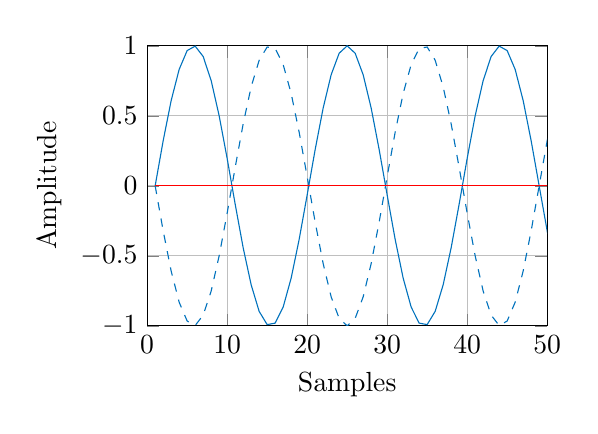
\begin{tikzpicture}

\begin{axis}[%
width=2in,
height=1.4in,
xlabel = {Samples},
ylabel = {Amplitude}, 
scale only axis,
xmin=0,
xmax=50,
xmajorgrids,
ymin=-1,
ymax=1,
ymajorgrids,
axis background/.style={fill=white}
]
\addplot [color=mycolor1,solid,forget plot]
  table[row sep=crcr]{%
1	0\\
2	0.321439465303162\\
3	0.608761429008721\\
4	0.831469612302545\\
5	0.965925826289068\\
6	0.997858923238603\\
7	0.923879532511287\\
8	0.751839807478978\\
9	0.5\\
10	0.195090322016128\\
11	-0.130526192220051\\
12	-0.442288690219001\\
13	-0.707106781186548\\
14	-0.896872741532688\\
15	-0.99144486137381\\
16	-0.98078528040323\\
17	-0.866025403784439\\
18	-0.659345815100069\\
19	-0.38268343236509\\
20	-0.0654031292301428\\
21	0.25881904510252\\
22	0.555570233019602\\
23	0.793353340291235\\
24	0.946930129495105\\
25	1\\
26	0.946930129495106\\
27	0.793353340291235\\
28	0.555570233019604\\
29	0.258819045102523\\
30	-0.0654031292301431\\
31	-0.38268343236509\\
32	-0.659345815100069\\
33	-0.866025403784438\\
34	-0.98078528040323\\
35	-0.991444861373811\\
36	-0.896872741532689\\
37	-0.707106781186547\\
38	-0.442288690219002\\
39	-0.130526192220051\\
40	0.195090322016127\\
41	0.499999999999999\\
42	0.751839807478976\\
43	0.923879532511286\\
44	0.997858923238604\\
45	0.965925826289069\\
46	0.831469612302546\\
47	0.608761429008723\\
48	0.321439465303162\\
49	-1.16403343982657e-15\\
50	-0.321439465303164\\
51	-0.608761429008723\\
52	-0.831469612302545\\
53	-0.965925826289068\\
54	-0.997858923238603\\
55	-0.923879532511286\\
56	-0.751839807478978\\
57	-0.5\\
58	-0.195090322016128\\
59	0.130526192220052\\
60	0.442288690218998\\
61	0.707106781186548\\
62	0.89687274153269\\
63	0.99144486137381\\
64	0.98078528040323\\
65	0.866025403784438\\
66	0.659345815100069\\
67	0.382683432365093\\
68	0.0654031292301461\\
69	-0.258819045102525\\
70	-0.555570233019603\\
71	-0.793353340291236\\
72	-0.946930129495106\\
73	-1\\
74	-0.946930129495105\\
75	-0.793353340291237\\
76	-0.555570233019604\\
77	-0.25881904510252\\
78	0.0654031292301442\\
79	0.382683432365091\\
80	0.65934581510007\\
81	0.866025403784439\\
82	0.98078528040323\\
83	0.991444861373811\\
84	0.896872741532689\\
85	0.707106781186549\\
86	0.442288690219003\\
87	0.13052619222005\\
88	-0.19509032201613\\
89	-0.499999999999999\\
90	-0.751839807478979\\
91	-0.923879532511286\\
92	-0.997858923238603\\
93	-0.965925826289069\\
94	-0.831469612302548\\
95	-0.608761429008722\\
96	-0.321439465303163\\
97	2.32806687965315e-15\\
};
\addplot [color=mycolor1,dashed,forget plot]
  table[row sep=crcr]{%
1	-0\\
2	-0.321439465303162\\
3	-0.608761429008721\\
4	-0.831469612302545\\
5	-0.965925826289068\\
6	-0.997858923238603\\
7	-0.923879532511287\\
8	-0.751839807478978\\
9	-0.5\\
10	-0.195090322016128\\
11	0.130526192220051\\
12	0.442288690219001\\
13	0.707106781186548\\
14	0.896872741532688\\
15	0.99144486137381\\
16	0.98078528040323\\
17	0.866025403784439\\
18	0.659345815100069\\
19	0.38268343236509\\
20	0.0654031292301428\\
21	-0.25881904510252\\
22	-0.555570233019602\\
23	-0.793353340291235\\
24	-0.946930129495105\\
25	-1\\
26	-0.946930129495106\\
27	-0.793353340291235\\
28	-0.555570233019604\\
29	-0.258819045102523\\
30	0.0654031292301431\\
31	0.38268343236509\\
32	0.659345815100069\\
33	0.866025403784438\\
34	0.98078528040323\\
35	0.991444861373811\\
36	0.896872741532689\\
37	0.707106781186547\\
38	0.442288690219002\\
39	0.130526192220051\\
40	-0.195090322016127\\
41	-0.499999999999999\\
42	-0.751839807478976\\
43	-0.923879532511286\\
44	-0.997858923238604\\
45	-0.965925826289069\\
46	-0.831469612302546\\
47	-0.608761429008723\\
48	-0.321439465303162\\
49	1.16403343982657e-15\\
50	0.321439465303164\\
51	0.608761429008723\\
52	0.831469612302545\\
53	0.965925826289068\\
54	0.997858923238603\\
55	0.923879532511286\\
56	0.751839807478978\\
57	0.5\\
58	0.195090322016128\\
59	-0.130526192220052\\
60	-0.442288690218998\\
61	-0.707106781186548\\
62	-0.89687274153269\\
63	-0.99144486137381\\
64	-0.98078528040323\\
65	-0.866025403784438\\
66	-0.659345815100069\\
67	-0.382683432365093\\
68	-0.0654031292301461\\
69	0.258819045102525\\
70	0.555570233019603\\
71	0.793353340291236\\
72	0.946930129495106\\
73	1\\
74	0.946930129495105\\
75	0.793353340291237\\
76	0.555570233019604\\
77	0.25881904510252\\
78	-0.0654031292301442\\
79	-0.382683432365091\\
80	-0.65934581510007\\
81	-0.866025403784439\\
82	-0.98078528040323\\
83	-0.991444861373811\\
84	-0.896872741532689\\
85	-0.707106781186549\\
86	-0.442288690219003\\
87	-0.13052619222005\\
88	0.19509032201613\\
89	0.499999999999999\\
90	0.751839807478979\\
91	0.923879532511286\\
92	0.997858923238603\\
93	0.965925826289069\\
94	0.831469612302548\\
95	0.608761429008722\\
96	0.321439465303163\\
97	-2.32806687965315e-15\\
};
\addplot [color=red,solid,forget plot]
  table[row sep=crcr]{%
1	0\\
2	0\\
3	0\\
4	0\\
5	0\\
6	0\\
7	0\\
8	0\\
9	0\\
10	0\\
11	0\\
12	0\\
13	0\\
14	0\\
15	0\\
16	0\\
17	0\\
18	0\\
19	0\\
20	0\\
21	0\\
22	0\\
23	0\\
24	0\\
25	0\\
26	0\\
27	0\\
28	0\\
29	0\\
30	0\\
31	0\\
32	0\\
33	0\\
34	0\\
35	0\\
36	0\\
37	0\\
38	0\\
39	0\\
40	0\\
41	0\\
42	0\\
43	0\\
44	0\\
45	0\\
46	0\\
47	0\\
48	0\\
49	0\\
50	0\\
51	0\\
52	0\\
53	0\\
54	0\\
55	0\\
56	0\\
57	0\\
58	0\\
59	0\\
60	0\\
61	0\\
62	0\\
63	0\\
64	0\\
65	0\\
66	0\\
67	0\\
68	0\\
69	0\\
70	0\\
71	0\\
72	0\\
73	0\\
74	0\\
75	0\\
76	0\\
77	0\\
78	0\\
79	0\\
80	0\\
81	0\\
82	0\\
83	0\\
84	0\\
85	0\\
86	0\\
87	0\\
88	0\\
89	0\\
90	0\\
91	0\\
92	0\\
93	0\\
94	0\\
95	0\\
96	0\\
97	0\\
};
\end{axis}
\end{tikzpicture}%
	 		%\caption{2500 Hz}
	 	\end{center}
		\end{column}
	\end{columns}
\end{frame}

\subsection{Feedforward system}
\begin{frame}{Feedforward ANC}
	\begin{columns}	
			\begin{column}{0.5\textwidth}
			\begin{itemize}
			\item 1: Reference microphone
			\item 2: Headphone loudspeaker
			\end{itemize}
			\end{column}		
	\begin{column}{0.5\textwidth} 
	\begin{itemize}
			\item 3: Error microphone
			\item 4: Digital signal Processor (DSP)
	\end{itemize}
	\end{column}	
	\end{columns}	
	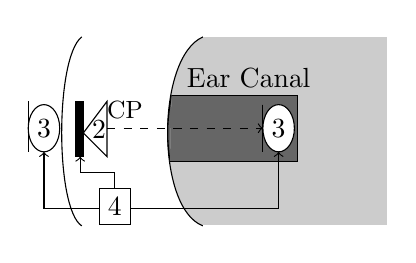
\begin{tikzpicture}
\draw [](-2.22,2.52) node (v1) {} .. controls (-2.56,2.26) and (-2.56,0.34) .. (-2.22,0.12) node (v2) {};

\draw [draw=black,fill=black!20](-0.68,2.52) node (v1) {} .. controls (-1.28,2.26) and (-1.28,0.34) .. (-0.68,0.12) node (v2) {};
\draw [white, fill=black!20](-0.68,2.52) -- (1.66,2.52) -- (1.66,0.12) -- (-0.68,0.12);


\draw [draw=black,fill=black!60](-1.08,1.78) node (v1) {} .. controls (-1.14,1.44) and (-1.14,1.24) .. (-1.1,0.94) node (v2) {};
\draw [draw=black,fill=black!60](-1.08,1.78) -- (0.52,1.78) -- (0.52,0.94) -- (-1.1,0.94);


\draw [draw=black,fill=white] (0.28,1.36) node (v3) {3} ellipse (0.2 and 0.3);
\draw [draw=black,fill=black](0.08,1.66) -- (0.08,1.06);

\draw [draw=black,fill=white] (-2.7,1.36) node (v3) {3} ellipse (0.2 and 0.3);
\draw [draw=black,fill=black](-2.9,1.7) -- (-2.9,1.06);


\draw [draw=black,fill=black] (-2.2,1.7) rectangle (-2.3,1);
\draw (-2.2,1.3) -- (-1.9,1.7) -- (-1.9,1) -- (-2.2,1.3);
\node at (-2,1.34) {2};


\draw[->,dashed] (-1.9,1.36) node[right=6.5,above]{\small{CP}}-- (0.08,1.36);
\draw  (-1.6,0.6) rectangle node{4}(-2,0.14);
\draw [->](-2,0.34) -- (-2.7,0.34) -- (-2.7,1.06);
\draw [->](-1.6,0.34) -- (0.28,0.34) -- (0.28,1.06);
\draw [->](-1.8,0.6) -- (-1.8,0.8) -- (-2.24,0.8) -- (-2.24,1);
\node at (-0.1,2) {Ear Canal};
\end{tikzpicture}
	\begin{itemize}
			\item Attenuate all kind of signals
			\item Process the signal upfront
			\item Delay of the system must be less than the propagation time
	\end{itemize}		
\end{frame}

\subsection{System delay}
\begin{frame}{Conversion delay}{Conversion delay}
	\begin{columns}
		\begin{column}{0.4\textwidth}
		\begin{itemize}
		\item Too much delay in converters
				\begin{itemize}
				\item $\Sigma \Delta$-converters
				\begin{itemize}
				\item Equivalent to 43 samples
				\end{itemize}								
				\end{itemize}
		\item TLV320AIC3204
				\begin{itemize}
				\item[\textcolor{MATLABred}{48 kHz}]= 900 $\mu S$ $\approx 31$ cm
				\item[\textcolor{MATLAByellow}{96 kHz}]= 450 $\mu S$ $\approx 15$ cm
				\item[\textcolor{MATLABpurple}{192 kHz}]= 225 $\mu S$ $\approx 8$ cm
				\end{itemize}	
				\item Mems 	microphone less delay	 
		\end{itemize}
		\end{column}
		\begin{column}{0.6\textwidth} 
		\begin{center}
		% This file was created by matlab2tikz.
%
%The latest updates can be retrieved from
%  http://www.mathworks.com/matlabcentral/fileexchange/22022-matlab2tikz-matlab2tikz
%where you can also make suggestions and rate matlab2tikz.
%
\definecolor{mycolor1}{rgb}{0.00000,0.44700,0.74100}%
\definecolor{mycolor2}{rgb}{0.85000,0.32500,0.09800}%
\definecolor{mycolor3}{rgb}{0.92900,0.69400,0.12500}%
\definecolor{mycolor4}{rgb}{0.49400,0.18400,0.55600}%
%
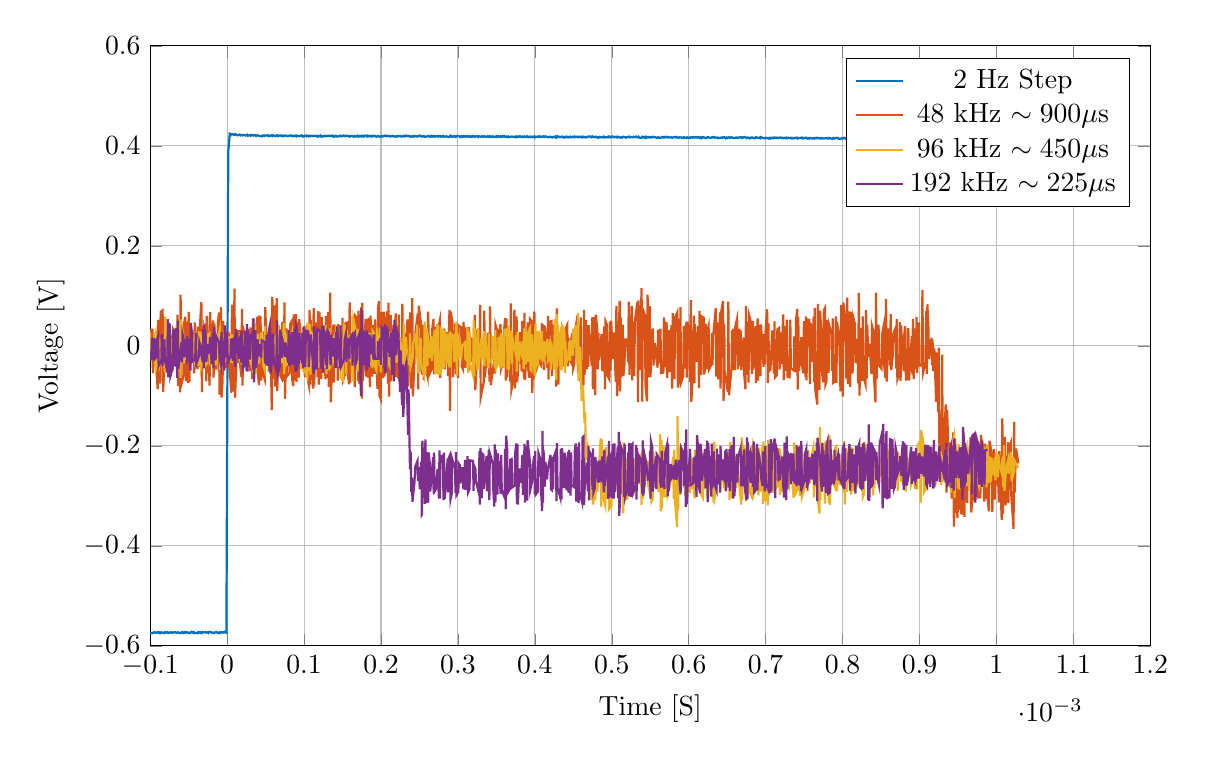
\begin{tikzpicture}

\begin{axis}[%
width=5in,
height=3in,
xmajorgrids,
xminorgrids,
ymajorgrids,
yminorgrids,
scale only axis,
xmin=-0.0001,
xmax=0.0012,
ymin=-0.6,
ymax=0.6,
ylabel={Voltage [V]},
xlabel={Time [S]},
axis background/.style={fill=white},
%legend style={legend cell align=left,align=left,draw=white!15!black}
]
\addplot [color=mycolor1,solid,thick]
  table[row sep=crcr]{%
-0.00010012	-0.5733\\
-0.00010012	-0.5733\\
-9.9069e-05	-0.5743\\
-9.6969e-05	-0.57464\\
-9.4869e-05	-0.57296\\
-9.4269e-05	-0.57263\\
-9.2169e-05	-0.5743\\
-9.2169e-05	-0.5743\\
-9.0519e-05	-0.57296\\
-8.8719e-05	-0.57296\\
-8.8119e-05	-0.57464\\
-8.6619e-05	-0.57464\\
-8.5719e-05	-0.57296\\
-8.4369e-05	-0.5733\\
-8.1969e-05	-0.57464\\
-8.1669e-05	-0.5743\\
-8.0619e-05	-0.57263\\
-7.8369e-05	-0.57363\\
-7.7619e-05	-0.57263\\
-7.5669e-05	-0.5743\\
-7.4169e-05	-0.57296\\
-7.3419e-05	-0.57263\\
-7.1619e-05	-0.57397\\
-7.1469e-05	-0.57397\\
-7.0719e-05	-0.57296\\
-6.8769e-05	-0.5733\\
-6.7569e-05	-0.57263\\
-6.5619e-05	-0.57397\\
-6.3969e-05	-0.57296\\
-6.3669e-05	-0.57296\\
-6.1119e-05	-0.57464\\
-6.0969e-05	-0.57464\\
-5.8869e-05	-0.57263\\
-5.7819e-05	-0.57296\\
-5.7369e-05	-0.5743\\
-5.5569e-05	-0.57263\\
-5.4519e-05	-0.57397\\
-5.3019e-05	-0.57263\\
-5.1969e-05	-0.57363\\
-5.0469e-05	-0.5733\\
-4.9419e-05	-0.57464\\
-4.8069e-05	-0.57397\\
-4.6419e-05	-0.57195\\
-4.5069e-05	-0.57229\\
-4.3719e-05	-0.5743\\
-4.2819e-05	-0.57296\\
-4.1919e-05	-0.57397\\
-3.8619e-05	-0.57464\\
-3.8019e-05	-0.5733\\
-3.7569e-05	-0.5743\\
-3.5769e-05	-0.57263\\
-3.4419e-05	-0.57296\\
-3.3819e-05	-0.5743\\
-3.2319e-05	-0.57263\\
-3.1869e-05	-0.57363\\
-2.8719e-05	-0.57229\\
-2.7369e-05	-0.57363\\
-2.7219e-05	-0.57363\\
-2.4819e-05	-0.57263\\
-2.4519e-05	-0.5733\\
-2.4369e-05	-0.57263\\
-2.1669e-05	-0.57229\\
-2.0919e-05	-0.57363\\
-1.8969e-05	-0.5733\\
-1.8369e-05	-0.5743\\
-1.6869e-05	-0.57397\\
-1.5219e-05	-0.57263\\
-1.3119e-05	-0.57263\\
-1.1919e-05	-0.5743\\
-9.8194e-06	-0.57464\\
-9.3694e-06	-0.5733\\
-8.7694e-06	-0.57397\\
-7.5694e-06	-0.57263\\
-6.2194e-06	-0.57263\\
-5.1694e-06	-0.57363\\
-3.2194e-06	-0.57195\\
-2.1694e-06	-0.57363\\
-9.6936e-07	-0.57397\\
1.4306e-06	0.38857\\
1.4306e-06	0.38857\\
3.3806e-06	0.4238\\
4.7306e-06	0.42212\\
5.0306e-06	0.42346\\
7.1306e-06	0.42313\\
8.7806e-06	0.42178\\
9.5306e-06	0.42178\\
1.0431e-05	0.42346\\
1.1781e-05	0.42212\\
1.2831e-05	0.42111\\
1.4331e-05	0.42111\\
1.5981e-05	0.42245\\
1.7331e-05	0.42111\\
1.7631e-05	0.42178\\
1.9731e-05	0.42078\\
2.0631e-05	0.42178\\
2.2131e-05	0.42145\\
2.3931e-05	0.42044\\
2.6031e-05	0.42212\\
2.6781e-05	0.42011\\
2.7981e-05	0.42044\\
2.9631e-05	0.42145\\
3.0081e-05	0.42145\\
3.0831e-05	0.42011\\
3.3081e-05	0.42178\\
3.4731e-05	0.42044\\
3.6231e-05	0.42145\\
3.7581e-05	0.41977\\
3.7731e-05	0.42011\\
3.9231e-05	0.42111\\
4.0431e-05	0.42078\\
4.1631e-05	0.41943\\
4.3581e-05	0.41977\\
4.4931e-05	0.41876\\
4.5531e-05	0.4191\\
4.6581e-05	0.42078\\
4.8231e-05	0.41977\\
4.8531e-05	0.42044\\
5.2281e-05	0.42078\\
5.3181e-05	0.41977\\
5.3481e-05	0.42044\\
5.3931e-05	0.41943\\
5.6181e-05	0.41977\\
5.7531e-05	0.42111\\
5.8731e-05	0.41977\\
5.9181e-05	0.42111\\
6.1131e-05	0.42044\\
6.2031e-05	0.41943\\
6.3831e-05	0.41943\\
6.4731e-05	0.42111\\
6.6681e-05	0.41943\\
6.7581e-05	0.42044\\
6.9831e-05	0.42078\\
7.0731e-05	0.41943\\
7.1781e-05	0.42044\\
7.3431e-05	0.4191\\
7.4481e-05	0.41943\\
7.4631e-05	0.42044\\
7.6731e-05	0.42044\\
7.8531e-05	0.4191\\
7.9431e-05	0.41943\\
8.1531e-05	0.42078\\
8.2281e-05	0.42078\\
8.4231e-05	0.41943\\
8.4531e-05	0.42011\\
8.5431e-05	0.4191\\
8.8881e-05	0.42044\\
8.9631e-05	0.4191\\
8.9781e-05	0.41943\\
9.0531e-05	0.42044\\
9.2481e-05	0.42011\\
9.3231e-05	0.4191\\
9.6081e-05	0.42044\\
9.7431e-05	0.41943\\
9.7581e-05	0.42011\\
9.8781e-05	0.41843\\
0.00010013	0.4191\\
0.00010118	0.42044\\
0.00010283	0.4191\\
0.00010358	0.42044\\
0.00010553	0.4191\\
0.00010598	0.42011\\
0.00010793	0.4191\\
0.00010838	0.42011\\
0.00011078	0.42011\\
0.00011183	0.4191\\
0.00011318	0.42011\\
0.00011573	0.4191\\
0.00011663	0.42011\\
0.00011798	0.41809\\
0.00011843	0.41843\\
0.00011948	0.41977\\
0.00012143	0.41876\\
0.00012188	0.42044\\
0.00012413	0.41843\\
0.00012623	0.42011\\
0.00012623	0.42011\\
0.00012803	0.4191\\
0.00012878	0.4191\\
0.00012908	0.42011\\
0.00013148	0.41943\\
0.00013253	0.42044\\
0.00013553	0.4191\\
0.00013643	0.42044\\
0.00013703	0.42044\\
0.00013853	0.41809\\
0.00013913	0.41876\\
0.00014093	0.42011\\
0.00014183	0.41977\\
0.00014213	0.41876\\
0.00014468	0.41876\\
0.00014663	0.41977\\
0.00014708	0.42011\\
0.00014753	0.4191\\
0.00014963	0.4191\\
0.00015113	0.42078\\
0.00015293	0.4191\\
0.00015473	0.42011\\
0.00015488	0.42044\\
0.00015698	0.4191\\
0.00015743	0.41977\\
0.00015953	0.41843\\
0.00015998	0.4191\\
0.00016148	0.41977\\
0.00016253	0.41977\\
0.00016448	0.41809\\
0.00016553	0.41977\\
0.00016763	0.41843\\
0.00016853	0.41843\\
0.00016943	0.42011\\
0.00017093	0.41843\\
0.00017153	0.41977\\
0.00017453	0.41843\\
0.00017528	0.42011\\
0.00017573	0.42044\\
0.00017768	0.41843\\
0.00017813	0.4191\\
0.00017888	0.42044\\
0.00018188	0.41876\\
0.00018233	0.42011\\
0.00018338	0.41876\\
0.00018473	0.42011\\
0.00018713	0.41843\\
0.00018818	0.41977\\
0.00018953	0.41876\\
0.00019058	0.42011\\
0.00019208	0.41977\\
0.00019388	0.41809\\
0.00019388	0.41809\\
0.00019598	0.41977\\
0.00019643	0.41977\\
0.00019868	0.41809\\
0.00019943	0.41843\\
0.00020048	0.41943\\
0.00020183	0.41876\\
0.00020198	0.41943\\
0.00020423	0.41943\\
0.00020498	0.42044\\
0.00020678	0.42011\\
0.00020708	0.4191\\
0.00021023	0.41977\\
0.00021203	0.41843\\
0.00021203	0.41843\\
0.00021383	0.41977\\
0.00021473	0.42011\\
0.00021593	0.41876\\
0.00021728	0.4191\\
0.00021923	0.41809\\
0.00021983	0.41843\\
0.00022088	0.41977\\
0.00022238	0.41876\\
0.00022358	0.41977\\
0.00022568	0.41977\\
0.00022613	0.41843\\
0.00022823	0.41843\\
0.00022958	0.42011\\
0.00023093	0.41876\\
0.00023258	0.42044\\
0.00023288	0.42044\\
0.00023468	0.4191\\
0.00023603	0.42011\\
0.00023738	0.41876\\
0.00023828	0.4191\\
0.00023903	0.41809\\
0.00024233	0.41977\\
0.00024293	0.41843\\
0.00024338	0.41876\\
0.00024473	0.41943\\
0.00024698	0.41843\\
0.00024803	0.41943\\
0.00024848	0.4191\\
0.00025058	0.42044\\
0.00025103	0.41943\\
0.00025298	0.41843\\
0.00025373	0.41876\\
0.00025418	0.41943\\
0.00025628	0.4191\\
0.00025643	0.41809\\
0.00025928	0.41843\\
0.00026138	0.41977\\
0.00026138	0.41977\\
0.00026333	0.41809\\
0.00026453	0.41843\\
0.00026513	0.42011\\
0.00026663	0.41977\\
0.00026708	0.41843\\
0.00026933	0.41977\\
0.00026978	0.41843\\
0.00027353	0.41943\\
0.00027443	0.41843\\
0.00027443	0.41843\\
0.00027518	0.41943\\
0.00027713	0.41843\\
0.00027728	0.41943\\
0.00027968	0.41843\\
0.00028088	0.41977\\
0.00028238	0.41809\\
0.00028478	0.4191\\
0.00028478	0.4191\\
0.00028673	0.41776\\
0.00028853	0.41776\\
0.00029003	0.42011\\
0.00029003	0.42011\\
0.00029078	0.41876\\
0.00029258	0.4191\\
0.00029288	0.41809\\
0.00029573	0.41943\\
0.00029708	0.41776\\
0.00029783	0.41843\\
0.00029858	0.41977\\
0.00030038	0.41977\\
0.00030278	0.41776\\
0.00030323	0.41742\\
0.00030458	0.41943\\
0.00030608	0.4191\\
0.00030623	0.41809\\
0.00030863	0.41943\\
0.00030938	0.41809\\
0.00031148	0.41943\\
0.00031283	0.41809\\
0.00031373	0.41943\\
0.00031553	0.41809\\
0.00031658	0.4191\\
0.00031793	0.41776\\
0.00031868	0.41843\\
0.00031973	0.41977\\
0.00032123	0.4191\\
0.00032153	0.41809\\
0.00032543	0.41943\\
0.00032633	0.41776\\
0.00032663	0.41843\\
0.00032783	0.4191\\
0.00032963	0.41809\\
0.00033128	0.4191\\
0.00033173	0.4191\\
0.00033263	0.41776\\
0.00033443	0.4191\\
0.00033653	0.41809\\
0.00033743	0.41776\\
0.00033863	0.4191\\
0.00033998	0.41776\\
0.00034133	0.4191\\
0.00034208	0.41876\\
0.00034253	0.41776\\
0.00034538	0.4191\\
0.00034643	0.41742\\
0.00034823	0.41776\\
0.00034988	0.4191\\
0.00035048	0.41809\\
0.00035108	0.41943\\
0.00035243	0.4191\\
0.00035363	0.41776\\
0.00035543	0.4191\\
0.00035618	0.41776\\
0.00035798	0.4191\\
0.00035828	0.41843\\
0.00036038	0.41943\\
0.00036128	0.41809\\
0.00036278	0.41876\\
0.00036458	0.41742\\
0.00036548	0.41843\\
0.00036578	0.41742\\
0.00036803	0.41776\\
0.00037028	0.41876\\
0.00037073	0.41843\\
0.00037283	0.41742\\
0.00037508	0.41876\\
0.00037583	0.41709\\
0.00037583	0.41709\\
0.00037808	0.41876\\
0.00037883	0.41776\\
0.00038063	0.4191\\
0.00038183	0.41843\\
0.00038258	0.41742\\
0.00038393	0.41843\\
0.00038513	0.41742\\
0.00038648	0.41876\\
0.00038873	0.41742\\
0.00038888	0.41742\\
0.00038993	0.4191\\
0.00039158	0.41742\\
0.00039368	0.41843\\
0.00039443	0.41742\\
0.00039578	0.41843\\
0.00039728	0.41742\\
0.00039923	0.41843\\
0.00039953	0.41776\\
0.00039968	0.41876\\
0.00040178	0.41776\\
0.00040448	0.41876\\
0.00040538	0.41776\\
0.00040688	0.4191\\
0.00040718	0.41876\\
0.00040793	0.41776\\
0.00041153	0.4191\\
0.00041213	0.41742\\
0.00041228	0.41742\\
0.00041288	0.41876\\
0.00041528	0.41843\\
0.00041588	0.41742\\
0.00041783	0.41709\\
0.00041978	0.41843\\
0.00042008	0.41809\\
0.00042218	0.41675\\
0.00042278	0.41675\\
0.00042398	0.41809\\
0.00042638	0.41675\\
0.00042698	0.41843\\
0.00042833	0.41642\\
0.00042938	0.4191\\
0.00043103	0.41843\\
0.00043268	0.41709\\
0.00043298	0.41709\\
0.00043508	0.41843\\
0.00043568	0.41843\\
0.00043748	0.41642\\
0.00043853	0.41675\\
0.00043928	0.41776\\
0.00044078	0.41709\\
0.00044123	0.41843\\
0.00044393	0.41675\\
0.00044573	0.41843\\
0.00044603	0.41843\\
0.00044693	0.41709\\
0.00044888	0.41742\\
0.00044948	0.41843\\
0.00045143	0.41709\\
0.00045203	0.41843\\
0.00045533	0.41809\\
0.00045623	0.41709\\
0.00045698	0.41709\\
0.00045713	0.41809\\
0.00045998	0.41809\\
0.00046133	0.41642\\
0.00046178	0.41642\\
0.00046253	0.41843\\
0.00046463	0.41776\\
0.00046583	0.41675\\
0.00046688	0.41709\\
0.00046898	0.41843\\
0.00046958	0.41776\\
0.00047063	0.41876\\
0.00047213	0.41876\\
0.00047348	0.41709\\
0.00047498	0.41876\\
0.00047573	0.41742\\
0.00047768	0.41809\\
0.00047933	0.41709\\
0.00048023	0.41809\\
0.00048248	0.41574\\
0.00048248	0.41574\\
0.00048413	0.41809\\
0.00048518	0.41776\\
0.00048623	0.41675\\
0.00048863	0.41809\\
0.00048983	0.41675\\
0.00049028	0.41809\\
0.00049118	0.41709\\
0.00049523	0.41709\\
0.00049538	0.41843\\
0.00049598	0.41876\\
0.00049763	0.41709\\
0.00049808	0.41776\\
0.00049853	0.41709\\
0.00050123	0.41876\\
0.00050213	0.41709\\
0.00050363	0.41709\\
0.00050498	0.41809\\
0.00050693	0.41675\\
0.00050708	0.41809\\
0.00050873	0.41809\\
0.00051113	0.41642\\
0.00051173	0.41608\\
0.00051308	0.41742\\
0.00051368	0.41675\\
0.00051488	0.41809\\
0.00051743	0.41742\\
0.00051833	0.41608\\
0.00051893	0.41675\\
0.00052028	0.41742\\
0.00052223	0.41843\\
0.00052328	0.41709\\
0.00052403	0.41809\\
0.00052643	0.41675\\
0.00052688	0.41709\\
0.00052823	0.41809\\
0.00052958	0.41742\\
0.00053168	0.41843\\
0.00053273	0.41709\\
0.00053453	0.41843\\
0.00053453	0.41843\\
0.00053528	0.41642\\
0.00053843	0.41608\\
0.00053948	0.41742\\
0.00053963	0.41675\\
0.00054158	0.41776\\
0.00054293	0.41608\\
0.00054428	0.41809\\
0.00054503	0.41608\\
0.00054698	0.41776\\
0.00054803	0.41776\\
0.00054878	0.41642\\
0.00055103	0.41776\\
0.00055193	0.41675\\
0.00055268	0.41675\\
0.00055403	0.41809\\
0.00055523	0.41776\\
0.00055688	0.41675\\
0.00055943	0.41574\\
0.00056048	0.41742\\
0.00056048	0.41742\\
0.00056243	0.41574\\
0.00056438	0.41642\\
0.00056573	0.41776\\
0.00056573	0.41776\\
0.00056783	0.41642\\
0.00056828	0.41675\\
0.00056858	0.41776\\
0.00057098	0.41675\\
0.00057158	0.41809\\
0.00057353	0.41742\\
0.00057443	0.41642\\
0.00057713	0.41709\\
0.00057833	0.41608\\
0.00057863	0.41642\\
0.00058118	0.41776\\
0.00058163	0.41742\\
0.00058358	0.41642\\
0.00058448	0.41776\\
0.00058598	0.41642\\
0.00058688	0.41574\\
0.00058823	0.41709\\
0.00059033	0.41675\\
0.00059138	0.41574\\
0.00059213	0.41574\\
0.00059378	0.41742\\
0.00059423	0.41709\\
0.00059483	0.41574\\
0.00059693	0.41574\\
0.00059783	0.41709\\
0.00059948	0.41574\\
0.00060143	0.41675\\
0.00060203	0.41608\\
0.00060368	0.41742\\
0.00060488	0.41642\\
0.00060563	0.41742\\
0.00060728	0.41642\\
0.00060893	0.41742\\
0.00061043	0.41709\\
0.00061133	0.41608\\
0.00061283	0.41742\\
0.00061478	0.41574\\
0.00061583	0.41709\\
0.00061658	0.41507\\
0.00061763	0.41574\\
0.00061853	0.41742\\
0.00062033	0.41675\\
0.00062123	0.41541\\
0.00062333	0.41574\\
0.00062423	0.41742\\
0.00062573	0.41709\\
0.00062813	0.41574\\
0.00062813	0.41574\\
0.00063053	0.41709\\
0.00063083	0.41675\\
0.00063173	0.41776\\
0.00063323	0.41742\\
0.00063383	0.41608\\
0.00063683	0.41675\\
0.00063788	0.41541\\
0.00063848	0.41608\\
0.00063923	0.41541\\
0.00064178	0.41541\\
0.00064223	0.41642\\
0.00064373	0.41574\\
0.00064448	0.41709\\
0.00064643	0.41709\\
0.00064778	0.41507\\
0.00064898	0.41675\\
0.00064988	0.41541\\
0.00065243	0.41742\\
0.00065348	0.41574\\
0.00065408	0.41608\\
0.00065543	0.41709\\
0.00065663	0.41675\\
0.00065738	0.41574\\
0.00066008	0.41541\\
0.00066173	0.41675\\
0.00066248	0.41642\\
0.00066353	0.41541\\
0.00066458	0.41541\\
0.00066473	0.41675\\
0.00066863	0.41709\\
0.00066938	0.41541\\
0.00066998	0.41574\\
0.00067178	0.41742\\
0.00067253	0.41776\\
0.00067478	0.41608\\
0.00067523	0.41541\\
0.00067658	0.41675\\
0.00067748	0.41642\\
0.00067958	0.41474\\
0.00068003	0.41541\\
0.00068093	0.41642\\
0.00068333	0.41642\\
0.00068438	0.41507\\
0.00068648	0.41507\\
0.00068723	0.41709\\
0.00068798	0.41709\\
0.00069023	0.41541\\
0.00069128	0.41541\\
0.00069293	0.41709\\
0.00069323	0.41608\\
0.00069368	0.41709\\
0.00069563	0.41642\\
0.00069698	0.41507\\
0.00069953	0.41507\\
0.00070088	0.41608\\
0.00070088	0.41608\\
0.00070328	0.41507\\
0.00070418	0.4144\\
0.00070553	0.41608\\
0.00070643	0.41474\\
0.00070793	0.41608\\
0.00070928	0.41608\\
0.00070958	0.41507\\
0.00071183	0.41541\\
0.00071198	0.41642\\
0.00071453	0.41541\\
0.00071498	0.41642\\
0.00071678	0.41541\\
0.00071858	0.41675\\
0.00071903	0.41675\\
0.00072068	0.41541\\
0.00072173	0.41608\\
0.00072308	0.41507\\
0.00072443	0.41608\\
0.00072638	0.41507\\
0.00072728	0.41642\\
0.00072848	0.41541\\
0.00072983	0.41608\\
0.00073028	0.41541\\
0.00073313	0.41608\\
0.00073418	0.41474\\
0.00073463	0.41541\\
0.00073523	0.41474\\
0.00073778	0.41574\\
0.00073808	0.41507\\
0.00074063	0.41642\\
0.00074168	0.4144\\
0.00074258	0.41507\\
0.00074273	0.41574\\
0.00074633	0.41608\\
0.00074663	0.41507\\
0.00074813	0.41474\\
0.00074858	0.41608\\
0.00075038	0.41507\\
0.00075263	0.41642\\
0.00075308	0.41574\\
0.00075413	0.4144\\
0.00075698	0.41574\\
0.00075713	0.41474\\
0.00075818	0.41541\\
0.00076028	0.4144\\
0.00076088	0.41474\\
0.00076178	0.41574\\
0.00076358	0.4144\\
0.00076448	0.41574\\
0.00076628	0.41507\\
0.00076658	0.41608\\
0.00076853	0.41574\\
0.00076988	0.41474\\
0.00077138	0.4144\\
0.00077183	0.41574\\
0.00077378	0.41541\\
0.00077453	0.4144\\
0.00077648	0.41474\\
0.00077858	0.41574\\
0.00077888	0.41541\\
0.00078023	0.4144\\
0.00078188	0.41474\\
0.00078203	0.41574\\
0.00078428	0.41507\\
0.00078623	0.41373\\
0.00078698	0.4144\\
0.00078803	0.41574\\
0.00078938	0.4144\\
0.00079148	0.41574\\
0.00079208	0.41608\\
0.00079403	0.41474\\
0.00079448	0.41507\\
0.00079508	0.41407\\
0.00079763	0.41373\\
0.00079853	0.41507\\
0.00079988	0.4144\\
0.00080198	0.41608\\
0.00080258	0.41574\\
0.00080378	0.41407\\
0.00080498	0.41541\\
0.00080738	0.4144\\
0.00080783	0.4144\\
0.00080813	0.41541\\
0.00081008	0.41507\\
0.00081128	0.41407\\
0.00081293	0.41507\\
0.00081398	0.4134\\
0.00081548	0.41507\\
0.00081683	0.41373\\
0.00081863	0.41373\\
0.00082013	0.41507\\
0.00082148	0.41407\\
0.00082223	0.41541\\
0.00082403	0.4134\\
0.00082538	0.41474\\
0.00082598	0.41407\\
0.00082658	0.41507\\
0.00082913	0.41407\\
0.00083048	0.41574\\
0.00083093	0.41474\\
0.00083198	0.41574\\
0.00083363	0.41474\\
0.00083438	0.41541\\
0.00083678	0.41608\\
0.00083798	0.41474\\
0.00083888	0.41541\\
0.00083963	0.41407\\
0.00084263	0.41541\\
0.00084293	0.41407\\
0.00084473	0.41373\\
0.00084638	0.41507\\
0.00084728	0.41407\\
0.00084743	0.41507\\
0.00084938	0.41574\\
0.00085103	0.41407\\
0.00085178	0.41407\\
0.00085238	0.41507\\
0.00085463	0.41474\\
0.00085658	0.41306\\
0.00085733	0.41306\\
0.00085823	0.41407\\
0.00085988	0.41373\\
0.00086168	0.41541\\
0.00086333	0.41541\\
0.00086423	0.41407\\
0.00086513	0.41407\\
0.00086603	0.41574\\
0.00086768	0.41373\\
0.00086978	0.41474\\
0.00086993	0.41373\\
0.00087128	0.41541\\
0.00087263	0.41474\\
0.00087293	0.41373\\
0.00087578	0.4144\\
0.00087728	0.4134\\
0.00087833	0.41306\\
0.00087893	0.4144\\
0.00088058	0.41373\\
0.00088283	0.41507\\
0.00088388	0.41474\\
0.00088523	0.41373\\
0.00088553	0.41407\\
0.00088778	0.41541\\
0.00088823	0.41574\\
0.00088988	0.41373\\
0.00089108	0.41507\\
0.00089333	0.41407\\
0.00089363	0.41474\\
0.00089558	0.41306\\
0.00089588	0.41373\\
0.00089648	0.41507\\
0.00089903	0.41474\\
0.00090053	0.4134\\
0.00090113	0.41474\\
0.00090128	0.41407\\
0.00090368	0.4144\\
0.00090473	0.41272\\
0.00090668	0.41373\\
0.00090788	0.41507\\
0.00090968	0.41306\\
0.00091118	0.41541\\
0.00091163	0.41541\\
0.00091403	0.41306\\
0.00091463	0.4144\\
0.00091553	0.41306\\
0.00091748	0.41373\\
0.00091763	0.4144\\
0.00092003	0.41474\\
0.00092048	0.4134\\
0.00092213	0.4144\\
0.00092258	0.4134\\
0.00092453	0.4134\\
0.00092618	0.41507\\
0.00092708	0.4144\\
0.00092888	0.4134\\
0.00093038	0.4134\\
0.00093098	0.41474\\
0.00093248	0.41407\\
0.00093443	0.41239\\
0.00093638	0.41239\\
0.00093758	0.4144\\
0.00093758	0.4144\\
0.00093848	0.41272\\
0.00094058	0.41306\\
0.00094178	0.4144\\
0.00094268	0.41306\\
0.00094283	0.4144\\
0.00094538	0.4144\\
0.00094598	0.41373\\
0.00094808	0.4134\\
0.00094898	0.41474\\
0.00095213	0.41474\\
0.00095258	0.41306\\
0.00095318	0.41373\\
0.00095408	0.41272\\
0.00095678	0.41272\\
0.00095813	0.41407\\
0.00095888	0.41507\\
0.00096053	0.41239\\
0.00096098	0.41306\\
0.00096248	0.41407\\
0.00096398	0.41407\\
0.00096473	0.41306\\
0.00096608	0.4134\\
0.00096743	0.41507\\
0.00096953	0.41507\\
0.00097058	0.4134\\
0.00097148	0.4144\\
0.00097283	0.41306\\
0.00097493	0.4134\\
0.00097658	0.41474\\
0.00097688	0.41474\\
0.00097868	0.41272\\
0.00097958	0.41239\\
0.00098093	0.41373\\
0.00098183	0.41407\\
0.00098348	0.41306\\
0.00098558	0.41306\\
0.00098648	0.4144\\
0.00098723	0.4134\\
0.00098828	0.4144\\
0.00098993	0.41306\\
0.00099173	0.41474\\
0.00099218	0.4144\\
0.00099368	0.41272\\
0.00099473	0.41306\\
0.00099713	0.4144\\
0.00099833	0.41407\\
0.00099953	0.41239\\
0.0010003	0.41239\\
0.0010013	0.41373\\
0.0010028	0.4144\\
0.0010045	0.41239\\
0.0010051	0.41272\\
0.0010061	0.41407\\
0.0010081	0.41407\\
0.0010099	0.41205\\
0.0010105	0.4134\\
0.0010115	0.41272\\
0.0010132	0.41239\\
0.0010142	0.41373\\
0.0010162	0.41306\\
0.0010181	0.4144\\
0.0010181	0.4144\\
0.0010184	0.41306\\
0.0010208	0.41407\\
0.0010226	0.41205\\
0.0010252	0.41239\\
0.0010259	0.41407\\
0.0010285	0.4134\\
};
\addlegendentry{2 Hz Step};

\addplot [color=mycolor2,solid,thick]
  table[row sep=crcr]{%
-0.00010012	-0.0041845\\
-9.9819e-05	0.033263\\
-9.7869e-05	-0.027255\\
-9.7119e-05	0.034266\\
-9.6519e-05	-0.054672\\
-9.3219e-05	0.0055117\\
-9.2169e-05	-0.032604\\
-9.0369e-05	-0.086769\\
-8.9619e-05	0.051987\\
-8.9619e-05	0.051987\\
-8.7069e-05	-0.075401\\
-8.7069e-05	-0.075401\\
-8.6469e-05	0.067701\\
-8.3919e-05	0.071045\\
-8.3169e-05	-0.092119\\
-8.1819e-05	-0.041632\\
-8.1219e-05	0.025238\\
-7.7169e-05	0.012867\\
-7.6569e-05	-0.021905\\
-7.5669e-05	0.033932\\
-7.4919e-05	-0.050994\\
-7.3869e-05	0.023232\\
-7.2669e-05	-0.040295\\
-7.1019e-05	-0.043972\\
-7.0119e-05	0.03226\\
-6.7119e-05	0.021895\\
-6.6369e-05	-0.041632\\
-6.4419e-05	0.062351\\
-6.3669e-05	-0.080082\\
-6.2769e-05	0.029919\\
-6.1269e-05	-0.092453\\
-6.0519e-05	0.10247\\
-5.9769e-05	-0.078411\\
-5.6469e-05	-0.05835\\
-5.5869e-05	0.045968\\
-5.4369e-05	0.058005\\
-5.3469e-05	-0.070386\\
-5.1519e-05	0.04764\\
-5.0919e-05	-0.074064\\
-5.0019e-05	0.068035\\
-4.9119e-05	-0.073061\\
-4.8069e-05	0.0346\\
-4.7169e-05	-0.031936\\
-4.3869e-05	0.025573\\
-4.2969e-05	-0.055006\\
-4.2819e-05	-0.040963\\
-4.2219e-05	0.046637\\
-3.8619e-05	-0.046647\\
-3.7869e-05	0.038278\\
-3.6969e-05	-0.041966\\
-3.6069e-05	0.022229\\
-3.3519e-05	0.087428\\
-3.2769e-05	-0.092453\\
-3.2469e-05	-0.042301\\
-3.1869e-05	0.036941\\
-2.7819e-05	0.04229\\
-2.7219e-05	-0.066374\\
-2.7069e-05	-0.070721\\
-2.6469e-05	0.059677\\
-2.2869e-05	-0.079414\\
-2.2119e-05	0.067367\\
-2.1969e-05	0.062351\\
-2.1069e-05	-0.037285\\
-1.8369e-05	0.050983\\
-1.7619e-05	-0.063365\\
-1.6719e-05	0.045634\\
-1.4169e-05	-0.045644\\
-1.4019e-05	-0.047316\\
-1.1919e-05	0.046303\\
-1.0569e-05	0.066698\\
-9.9694e-06	-0.097469\\
-8.0194e-06	0.077397\\
-7.2694e-06	-0.10349\\
-5.9194e-06	-0.06838\\
-5.3194e-06	0.049646\\
-3.8194e-06	0.015877\\
-1.8694e-06	-0.044307\\
-9.6936e-07	0.028916\\
1.1306e-06	-0.035279\\
1.8806e-06	0.028248\\
2.7806e-06	-0.041632\\
5.4806e-06	-0.093791\\
6.2306e-06	0.082413\\
8.6306e-06	-0.091785\\
9.2306e-06	0.072048\\
9.5306e-06	0.11418\\
1.0281e-05	-0.10382\\
1.3431e-05	0.031257\\
1.4181e-05	-0.034611\\
1.6281e-05	0.031925\\
1.7031e-05	-0.040629\\
1.8531e-05	-0.062362\\
1.9281e-05	0.073719\\
2.0031e-05	-0.079414\\
2.0781e-05	0.035269\\
2.2281e-05	0.027913\\
2.3331e-05	-0.028592\\
2.6031e-05	-0.02692\\
2.6781e-05	0.022229\\
2.8581e-05	0.019554\\
2.9481e-05	-0.050325\\
3.0231e-05	0.036606\\
3.2631e-05	-0.060021\\
3.2781e-05	-0.066708\\
3.3531e-05	0.054996\\
3.5631e-05	-0.036617\\
3.7581e-05	0.034266\\
3.9381e-05	0.058339\\
4.0131e-05	-0.059018\\
4.1331e-05	-0.078411\\
4.2081e-05	0.058339\\
4.3431e-05	0.057336\\
4.4181e-05	-0.069383\\
4.5981e-05	0.028582\\
4.6581e-05	-0.055675\\
4.8831e-05	-0.067043\\
4.9581e-05	0.077397\\
5.1681e-05	-0.023243\\
5.3331e-05	0.02691\\
5.4231e-05	-0.051662\\
5.6031e-05	0.042959\\
5.7981e-05	-0.12856\\
5.8581e-05	0.085087\\
5.8731e-05	0.097793\\
6.0681e-05	-0.066708\\
6.1431e-05	0.081075\\
6.2181e-05	-0.08142\\
6.4431e-05	0.095452\\
6.5181e-05	-0.090447\\
6.7131e-05	0.03995\\
6.7731e-05	-0.05534\\
7.0881e-05	-0.065037\\
7.1631e-05	0.047974\\
7.1631e-05	0.047974\\
7.3731e-05	-0.070386\\
7.4481e-05	0.086759\\
7.5231e-05	-0.10583\\
7.7181e-05	0.034935\\
7.7781e-05	-0.06069\\
8.1231e-05	-0.054337\\
8.1981e-05	0.043628\\
8.3931e-05	0.048977\\
8.4531e-05	-0.067711\\
8.6031e-05	-0.080751\\
8.6631e-05	0.06302\\
8.8881e-05	-0.069383\\
8.9481e-05	0.063355\\
9.0231e-05	-0.072058\\
9.0831e-05	0.04764\\
9.2931e-05	-0.063699\\
9.3681e-05	0.053324\\
9.5181e-05	0.028248\\
9.5931e-05	-0.037954\\
9.9081e-05	0.036941\\
9.9681e-05	-0.039626\\
0.00010043	0.039616\\
0.00010103	-0.062362\\
0.00010433	0.042959\\
0.00010508	-0.070052\\
0.00010643	-0.080082\\
0.00010718	0.071379\\
0.00010793	-0.077408\\
0.00010853	0.051652\\
0.00011183	-0.085432\\
0.00011243	0.075391\\
0.00011318	-0.078411\\
0.00011543	0.046971\\
0.00011753	-0.062362\\
0.00011828	0.069373\\
0.00011918	-0.077742\\
0.00012008	0.066698\\
0.00012218	-0.066708\\
0.00012293	0.057336\\
0.00012368	-0.054003\\
0.00012428	0.035269\\
0.00012788	-0.067043\\
0.00012863	0.059677\\
0.00012938	-0.064033\\
0.00013133	0.067701\\
0.00013208	-0.082088\\
0.00013403	0.10649\\
0.00013403	0.10649\\
0.00013478	-0.11285\\
0.00013808	0.041956\\
0.00013883	-0.073395\\
0.00013958	0.042625\\
0.00014018	-0.043304\\
0.00014303	0.034935\\
0.00014378	-0.069383\\
0.00014453	0.043293\\
0.00014543	-0.02993\\
0.00014753	0.024235\\
0.00014933	-0.032939\\
0.00014993	0.055664\\
0.00015068	-0.06838\\
0.00015323	-0.057346\\
0.00015383	0.0453\\
0.00015653	0.046971\\
0.00015713	-0.060021\\
0.00015848	-0.077073\\
0.00015923	0.086759\\
0.00015998	-0.074064\\
0.00016058	0.024235\\
0.00016388	-0.059687\\
0.00016493	0.041622\\
0.00016583	-0.082757\\
0.00016658	0.060011\\
0.00016943	0.054327\\
0.00017003	-0.070052\\
0.00017078	0.070376\\
0.00017168	-0.075736\\
0.00017438	0.077397\\
0.00017513	-0.10549\\
0.00017573	0.085756\\
0.00017648	-0.070052\\
0.00017993	0.053658\\
0.00018068	-0.061693\\
0.00018248	0.052655\\
0.00018308	-0.063365\\
0.00018368	0.055664\\
0.00018563	-0.082423\\
0.00018638	0.060345\\
0.00018863	-0.061359\\
0.00018863	-0.061359\\
0.00018938	0.041622\\
0.00019148	-0.056009\\
0.00019223	0.05299\\
0.00019538	-0.086101\\
0.00019613	0.077063\\
0.00019748	0.0891\\
0.00019808	-0.099809\\
0.00019958	-0.10583\\
0.00020033	0.067701\\
0.00020273	-0.064702\\
0.00020363	0.06837\\
0.00020438	-0.061693\\
0.00020648	0.052321\\
0.00020828	0.069373\\
0.00020903	-0.075736\\
0.00020978	0.086425\\
0.00021053	-0.10148\\
0.00021263	0.061683\\
0.00021338	-0.070386\\
0.00021458	0.0095239\\
0.00021503	-0.022908\\
0.00021923	0.064692\\
0.00021983	-0.062362\\
0.00022043	0.034266\\
0.00022238	-0.065371\\
0.00022298	0.062351\\
0.00022373	-0.068714\\
0.00022703	-0.078411\\
0.00022763	0.078066\\
0.00022778	0.084084\\
0.00022853	-0.077073\\
0.00023063	0.024235\\
0.00023138	-0.038623\\
0.00023438	0.052655\\
0.00023513	-0.081085\\
0.00023543	-0.03762\\
0.00023798	0.067032\\
0.00023888	-0.085766\\
0.00024068	0.095452\\
0.00024068	0.095452\\
0.00024143	-0.10115\\
0.00024323	-0.043638\\
0.00024488	0.027245\\
0.00024773	0.064692\\
0.00024848	-0.087104\\
0.00024848	-0.087104\\
0.00024908	0.080072\\
0.00025208	0.042959\\
0.00025283	-0.057346\\
0.00025478	0.041622\\
0.00025553	-0.068046\\
0.00025628	0.041622\\
0.00025688	-0.033607\\
0.00026063	-0.061693\\
0.00026123	0.06837\\
0.00026138	0.056333\\
0.00026318	-0.055675\\
0.00026558	-0.047316\\
0.00026633	0.030254\\
0.00026828	0.053993\\
0.00026903	-0.057012\\
0.00026918	-0.052331\\
0.00027128	0.037609\\
0.00027203	-0.04765\\
0.00027293	0.02457\\
0.00027638	0.050315\\
0.00027698	-0.048653\\
0.00027713	-0.064033\\
0.00027788	0.023567\\
0.00028118	-0.042969\\
0.00028193	0.0346\\
0.00028298	-0.047316\\
0.00028373	0.026241\\
0.00028628	0.025238\\
0.00028718	-0.060356\\
0.00028898	0.072048\\
0.00028973	-0.1299\\
0.00029003	-0.056009\\
0.00029048	0.06837\\
0.00029288	0.048309\\
0.00029363	-0.062696\\
0.00029678	0.045968\\
0.00029753	-0.057012\\
0.00029813	0.041622\\
0.00030008	-0.064702\\
0.00030038	-0.02993\\
0.00030083	0.040953\\
0.00030428	0.036606\\
0.00030503	-0.041298\\
0.00030653	-0.046647\\
0.00030728	0.04764\\
0.00030968	-0.043972\\
0.00031058	0.036606\\
0.00031088	0.020557\\
0.00031178	-0.035279\\
0.00031403	0.037275\\
0.00031478	-0.049656\\
0.00031688	0.01688\\
0.00031763	-0.032604\\
0.00032033	0.015877\\
0.00032108	-0.036951\\
0.00032183	0.062017\\
0.00032258	-0.088776\\
0.00032393	-0.048653\\
0.00032453	0.032929\\
0.00032813	-0.031936\\
0.00032888	0.082078\\
0.00032903	0.052655\\
0.00032963	-0.10282\\
0.00033353	-0.072392\\
0.00033428	0.070376\\
0.00033428	0.070376\\
0.00033503	-0.063365\\
0.00033683	-0.030933\\
0.00033878	0.026241\\
0.00034118	-0.071389\\
0.00034178	0.078735\\
0.00034208	0.050983\\
0.00034268	-0.078745\\
0.00034673	-0.033942\\
0.00034718	0.01922\\
0.00034808	-0.05534\\
0.00034883	0.04229\\
0.00035168	0.027913\\
0.00035243	-0.034611\\
0.00035243	-0.034611\\
0.00035318	0.021895\\
0.00035543	0.043293\\
0.00035618	-0.045644\\
0.00035903	-0.030264\\
0.00035978	0.027579\\
0.00036143	0.055664\\
0.00036218	-0.069383\\
0.00036308	0.054327\\
0.00036398	-0.06303\\
0.00036728	0.028248\\
0.00036803	-0.071389\\
0.00036878	0.085087\\
0.00036953	-0.088441\\
0.00037268	-0.064033\\
0.00037328	0.064358\\
0.00037343	0.072382\\
0.00037418	-0.085098\\
0.00037628	0.059008\\
0.00037703	-0.073061\\
0.00037853	-0.038623\\
0.00038063	0.027245\\
0.00038288	-0.051662\\
0.00038363	0.04998\\
0.00038363	0.04998\\
0.00038588	-0.065705\\
0.00038648	0.066029\\
0.00038723	-0.068714\\
0.00039083	0.046971\\
0.00039143	-0.046982\\
0.00039293	-0.064033\\
0.00039368	0.053658\\
0.00039578	0.049312\\
0.00039653	-0.094125\\
0.00039668	-0.091116\\
0.00039923	0.066698\\
0.00039938	0.06837\\
0.00040013	-0.05534\\
0.00040388	-0.038957\\
0.00040448	0.025907\\
0.00040463	0.027579\\
0.00040538	-0.03227\\
0.00040838	-0.03996\\
0.00040913	0.042625\\
0.00041123	0.03995\\
0.00041213	-0.048653\\
0.00041228	-0.038623\\
0.00041288	0.040284\\
0.00041633	-0.044307\\
0.00041708	0.059677\\
0.00041783	-0.067711\\
0.00041843	0.04764\\
0.00042158	0.049646\\
0.00042233	-0.06069\\
0.00042323	0.042959\\
0.00042398	-0.045978\\
0.00042713	0.052655\\
0.00042773	-0.08142\\
0.00042788	-0.078411\\
0.00042848	0.074722\\
0.00043058	-0.077742\\
0.00043133	0.025573\\
0.00043373	-0.04531\\
0.00043553	0.0346\\
0.00043568	0.034266\\
0.00043643	-0.037285\\
0.00043883	-0.040295\\
0.00043958	0.032929\\
0.00044213	0.041956\\
0.00044288	-0.040963\\
0.00044363	0.016545\\
0.00044453	-0.024914\\
0.00044648	-0.030933\\
0.00044723	0.011864\\
0.00044888	0.025907\\
0.00044978	-0.04531\\
0.00045128	-0.036617\\
0.00045203	0.025573\\
0.00045548	0.061348\\
0.00045623	-0.054672\\
0.00045803	0.040284\\
0.00045878	-0.071055\\
0.00045953	0.057002\\
0.00046013	-0.053669\\
0.00046313	-0.078076\\
0.00046388	0.072048\\
0.00046463	-0.058684\\
0.00046658	0.051652\\
0.00046748	-0.046982\\
0.00046838	0.033932\\
0.00046943	-0.042301\\
0.00047003	0.041287\\
0.00047393	-0.03996\\
0.00047468	0.056667\\
0.00047543	-0.086435\\
0.00047618	0.057336\\
0.00047843	-0.098472\\
0.00047918	0.062351\\
0.00048113	0.032594\\
0.00048188	-0.046982\\
0.00048263	0.025238\\
0.00048338	-0.028927\\
0.00048683	0.023901\\
0.00048773	-0.050659\\
0.00048773	-0.050659\\
0.00049028	0.038612\\
0.00049118	-0.087104\\
0.00049193	0.048977\\
0.00049373	0.04229\\
0.00049448	-0.059687\\
0.00049688	-0.067043\\
0.00049763	0.04764\\
0.00049838	-0.049656\\
0.00049913	0.050315\\
0.00050168	-0.026252\\
0.00050273	0.026576\\
0.00050528	-0.072058\\
0.00050588	0.062017\\
0.00050603	0.079738\\
0.00050693	-0.10081\\
0.00051023	0.089768\\
0.00051083	-0.091116\\
0.00051158	0.057002\\
0.00051218	-0.06303\\
0.00051428	0.04229\\
0.00051503	-0.060021\\
0.00051653	-0.03762\\
0.00051728	0.012533\\
0.00051983	0.012533\\
0.00052133	-0.032939\\
0.00052208	0.088431\\
0.00052298	-0.05835\\
0.00052583	0.079738\\
0.00052658	-0.069049\\
0.00052673	-0.064033\\
0.00052733	0.048643\\
0.00052928	-0.060356\\
0.00053003	0.049646\\
0.00053333	0.087428\\
0.00053408	-0.11251\\
0.00053483	0.090771\\
0.00053618	-0.048319\\
0.00053873	0.11518\\
0.00053963	-0.11151\\
0.00053963	-0.11151\\
0.00054038	0.073051\\
0.00054308	0.061683\\
0.00054383	-0.078411\\
0.00054578	-0.11084\\
0.00054653	0.10247\\
0.00054878	-0.06303\\
0.00054953	0.079403\\
0.00055043	-0.062362\\
0.00055133	0.016211\\
0.00055343	0.0346\\
0.00055418	-0.039626\\
0.00055598	0.0055117\\
0.00055793	-0.023911\\
0.00055958	-0.043638\\
0.00056018	0.032594\\
0.00056108	-0.034945\\
0.00056303	0.017548\\
0.00056333	0.034266\\
0.00056408	-0.054337\\
0.00056708	-0.053334\\
0.00056783	0.056667\\
0.00056963	0.012533\\
0.00057038	-0.042969\\
0.00057128	0.04764\\
0.00057203	-0.064033\\
0.00057488	0.031925\\
0.00057578	-0.052666\\
0.00057758	0.041287\\
0.00057848	-0.085766\\
0.00057863	-0.071389\\
0.00057923	0.065361\\
0.00058148	-0.066374\\
0.00058223	0.057002\\
0.00058508	0.066698\\
0.00058598	-0.08376\\
0.00058658	0.054327\\
0.00058853	-0.077073\\
0.00058928	0.077397\\
0.00059003	-0.07373\\
0.00059288	-0.06069\\
0.00059363	0.03995\\
0.00059603	-0.04531\\
0.00059678	0.046637\\
0.00059753	-0.063699\\
0.00059843	0.048643\\
0.00060098	0.015877\\
0.00060173	-0.072727\\
0.00060263	0.09144\\
0.00060338	-0.11218\\
0.00060488	-0.075067\\
0.00060668	0.060345\\
0.00060743	-0.074398\\
0.00060818	0.043293\\
0.00061058	-0.031936\\
0.00061253	0.03995\\
0.00061328	-0.084763\\
0.00061403	0.070042\\
0.00061613	-0.058684\\
0.00061673	0.059008\\
0.00061943	0.056333\\
0.00062003	-0.057346\\
0.00062138	-0.044641\\
0.00062228	0.044296\\
0.00062333	-0.047316\\
0.00062423	0.028916\\
0.00062588	0.039281\\
0.00062663	-0.046647\\
0.00062963	-0.036951\\
0.00063023	0.025238\\
0.00063098	-0.038957\\
0.00063158	0.015542\\
0.00063518	0.075057\\
0.00063593	-0.061359\\
0.00063758	0.046971\\
0.00063833	-0.067043\\
0.00063848	-0.065371\\
0.00064073	0.067032\\
0.00064148	-0.085432\\
0.00064208	0.066364\\
0.00064463	0.089434\\
0.00064538	-0.11051\\
0.00064628	0.042959\\
0.00064673	-0.050659\\
0.00065078	-0.091785\\
0.00065153	0.088431\\
0.00065153	0.088431\\
0.00065243	-0.098806\\
0.00065573	-0.042969\\
0.00065633	0.030922\\
0.00065708	-0.048653\\
0.00065783	0.034266\\
0.00065993	-0.048653\\
0.00066053	0.038278\\
0.00066293	0.054661\\
0.00066383	-0.046982\\
0.00066608	0.034266\\
0.00066683	-0.039291\\
0.00066758	0.030588\\
0.00066818	-0.048653\\
0.00067133	0.016545\\
0.00067208	-0.05534\\
0.00067373	-0.086769\\
0.00067448	0.079403\\
0.00067523	-0.058015\\
0.00067703	0.04764\\
0.00067778	-0.073395\\
0.00067853	0.061014\\
0.00068018	0.051652\\
0.00068228	-0.056009\\
0.00068318	0.049646\\
0.00068393	-0.04765\\
0.00068678	0.039616\\
0.00068753	-0.074398\\
0.00068963	0.054996\\
0.00069023	-0.069717\\
0.00069098	0.04229\\
0.00069308	-0.054672\\
0.00069323	-0.06069\\
0.00069398	0.042625\\
0.00069728	-0.041966\\
0.00069803	0.023567\\
0.00069878	-0.03762\\
0.00069953	0.020557\\
0.00070193	0.073051\\
0.00070283	-0.074733\\
0.00070358	0.0453\\
0.00070448	-0.050325\\
0.00070628	-0.046982\\
0.00070868	0.030922\\
0.00070868	0.030922\\
0.00071078	-0.05534\\
0.00071153	0.048977\\
0.00071213	-0.063365\\
0.00071438	-0.059018\\
0.00071528	0.033263\\
0.00071738	0.035603\\
0.00071813	-0.047316\\
0.00071993	0.026576\\
0.00072068	-0.036617\\
0.00072278	0.062686\\
0.00072353	-0.06838\\
0.00072458	0.039281\\
0.00072683	-0.050325\\
0.00072758	0.052321\\
0.00072833	-0.061693\\
0.00073118	-0.06303\\
0.00073208	0.052321\\
0.00073208	0.052321\\
0.00073283	-0.044975\\
0.00073673	-0.049322\\
0.00073733	0.018886\\
0.00073883	-0.052331\\
0.00073958	0.052655\\
0.00074108	0.073719\\
0.00074168	-0.087772\\
0.00074243	0.057336\\
0.00074348	-0.050325\\
0.00074648	0.017548\\
0.00074738	-0.039291\\
0.00074903	-0.055006\\
0.00074978	0.049312\\
0.00075188	-0.062362\\
0.00075248	0.058674\\
0.00075323	-0.069049\\
0.00075398	0.052655\\
0.00075683	0.051987\\
0.00075758	-0.076405\\
0.00075848	0.046303\\
0.00075983	-0.031936\\
0.00076253	0.058674\\
0.00076313	-0.073061\\
0.00076388	0.07606\\
0.00076448	-0.086435\\
0.00076718	-0.11753\\
0.00076793	0.08375\\
0.00077003	-0.088107\\
0.00077078	0.070376\\
0.00077258	0.024235\\
0.00077348	-0.057012\\
0.00077498	-0.073061\\
0.00077573	0.071713\\
0.00077708	0.075726\\
0.00077783	-0.077408\\
0.00077918	-0.071389\\
0.00077978	0.051987\\
0.00078188	-0.054003\\
0.00078263	0.040953\\
0.00078578	0.023232\\
0.00078653	-0.050325\\
0.00078728	0.054661\\
0.00078803	-0.074064\\
0.00079073	-0.071055\\
0.00079133	0.059008\\
0.00079208	-0.074064\\
0.00079283	0.04764\\
0.00079553	0.021226\\
0.00079718	-0.082757\\
0.00079733	-0.091116\\
0.00079838	0.081744\\
0.00080033	-0.10182\\
0.00080108	0.086759\\
0.00080393	0.038947\\
0.00080498	-0.065705\\
0.00080603	0.096121\\
0.00080693	-0.076739\\
0.00080918	0.069038\\
0.00080993	-0.082088\\
0.00081008	-0.057681\\
0.00081068	0.067701\\
0.00081308	-0.05534\\
0.00081398	0.057002\\
0.00081593	0.044965\\
0.00081683	-0.034611\\
0.00081938	0.014205\\
0.00082028	-0.075067\\
0.00082118	0.10582\\
0.00082193	-0.099475\\
0.00082463	0.035938\\
0.00082553	-0.070052\\
0.00082628	0.059008\\
0.00082703	-0.06069\\
0.00082988	-0.077073\\
0.00083063	0.071379\\
0.00083138	-0.065705\\
0.00083213	0.041956\\
0.00083348	-0.022574\\
0.00083513	0.0041743\\
0.00083753	-0.056678\\
0.00083828	0.039616\\
0.00083993	0.029585\\
0.00084068	-0.054337\\
0.00084278	-0.11318\\
0.00084353	0.10615\\
0.00084428	-0.066708\\
0.00084518	0.022898\\
0.00084683	0.04229\\
0.00084773	-0.03996\\
0.00085073	-0.045978\\
0.00085148	0.023901\\
0.00085358	0.040953\\
0.00085433	-0.041632\\
0.00085583	-0.065037\\
0.00085658	0.094115\\
0.00085733	-0.071724\\
0.00085958	0.034935\\
0.00085958	0.034935\\
0.00086183	-0.039626\\
0.00086258	0.063355\\
0.00086333	-0.048653\\
0.00086528	-0.020233\\
0.00086618	0.025573\\
0.00086903	0.035938\\
0.00086978	-0.045644\\
0.00087053	0.053324\\
0.00087128	-0.067043\\
0.00087398	-0.053669\\
0.00087473	0.047306\\
0.00087548	-0.070052\\
0.00087608	0.040619\\
0.00087953	-0.050659\\
0.00088028	0.023232\\
0.00088163	0.038947\\
0.00088238	-0.067377\\
0.00088478	-0.06604\\
0.00088553	0.035603\\
0.00088553	0.035603\\
0.00088643	-0.069383\\
0.00089003	0.01922\\
0.00089078	-0.056343\\
0.00089153	0.053658\\
0.00089243	-0.066708\\
0.00089468	0.034935\\
0.00089543	-0.046647\\
0.00089618	0.058005\\
0.00089708	-0.054672\\
0.00089918	0.046971\\
0.00089993	-0.039626\\
0.00090323	-0.039626\\
0.00090368	0.085756\\
0.00090383	0.11117\\
0.00090473	-0.053669\\
0.00090803	-0.03227\\
0.00090878	0.069373\\
0.00090953	-0.056678\\
0.00091028	0.083081\\
0.00091163	0.037275\\
0.00091238	-0.026586\\
0.00091568	0.016211\\
0.00091643	-0.039291\\
0.00091703	0.011864\\
0.00091793	-0.050325\\
0.00091928	-0.0051876\\
0.00092168	-0.11218\\
0.00092243	-0.013212\\
0.00092438	-0.13291\\
0.00092498	-0.0035158\\
0.00092588	-0.20212\\
0.00092873	-0.23489\\
0.00092948	-0.017559\\
0.00092978	-0.095797\\
0.00093038	-0.23689\\
0.00093413	-0.1172\\
0.00093488	-0.27702\\
0.00093503	-0.2934\\
0.00093593	-0.1289\\
0.00093923	-0.28303\\
0.00093998	-0.19309\\
0.00094013	-0.20379\\
0.00094193	-0.30577\\
0.00094388	-0.17337\\
0.00094478	-0.36161\\
0.00094703	-0.21416\\
0.00094793	-0.33419\\
0.00094853	-0.22185\\
0.00094928	-0.34455\\
0.00095198	-0.25094\\
0.00095273	-0.32784\\
0.00095348	-0.21616\\
0.00095423	-0.33486\\
0.00095723	-0.33586\\
0.00095783	-0.21483\\
0.00095843	-0.34188\\
0.00095918	-0.20045\\
0.00096203	-0.31446\\
0.00096308	-0.2048\\
0.00096548	-0.28805\\
0.00096608	-0.20513\\
0.00096638	-0.18273\\
0.00096713	-0.33319\\
0.00096983	-0.29741\\
0.00097073	-0.21449\\
0.00097193	-0.30911\\
0.00097268	-0.18774\\
0.00097553	-0.19176\\
0.00097628	-0.30577\\
0.00097703	-0.19309\\
0.00097913	-0.3051\\
0.00097913	-0.3051\\
0.00097988	-0.17838\\
0.00098273	-0.20981\\
0.00098408	-0.31145\\
0.00098483	-0.19543\\
0.00098603	-0.30644\\
0.00098693	-0.20413\\
0.00098753	-0.28838\\
0.00099023	-0.33085\\
0.00099113	-0.18975\\
0.00099398	-0.2175\\
0.00099473	-0.33185\\
0.00099473	-0.33185\\
0.00099683	-0.20647\\
0.00099773	-0.30778\\
0.00099848	-0.23255\\
0.0010018	-0.28069\\
0.0010024	-0.22887\\
0.001003	-0.31313\\
0.0010037	-0.21048\\
0.0010069	-0.3479\\
0.0010076	-0.14528\\
0.0010078	-0.15832\\
0.0010084	-0.33586\\
0.0010108	-0.18239\\
0.0010117	-0.31914\\
0.001013	-0.3051\\
0.0010151	-0.19242\\
0.0010157	-0.3148\\
0.0010166	-0.20379\\
0.0010186	-0.19477\\
0.0010192	-0.29574\\
0.0010223	-0.36595\\
0.0010231	-0.1523\\
0.0010237	-0.29373\\
0.0010256	-0.20513\\
0.0010285	-0.23522\\
};
\addlegendentry{48 kHz $\sim 900 \mu $s};

\addplot [color=mycolor3,solid,thick]
  table[row sep=crcr]{%
-0.00017139	0.020735\\
-0.00017079	-0.044798\\
-0.00017019	0.026753\\
-0.00016854	0.0023454\\
-0.00016809	-0.027746\\
-0.00016449	-0.048142\\
-0.00016389	0.0311\\
-0.00016164	-0.035771\\
-0.00016089	0.026419\\
-0.00015834	-0.058172\\
-0.00015774	0.072225\\
-0.00015699	-0.070878\\
-0.00015639	0.033774\\
-0.00015429	-0.052488\\
-0.00015369	0.034443\\
-0.00015174	-0.040786\\
-0.00015099	0.027087\\
-0.00014724	-0.032427\\
-0.00014649	0.010035\\
-0.00014574	-0.035771\\
-0.00014514	0.019732\\
-0.00014334	0.0080294\\
-0.00014259	-0.027078\\
-0.00013899	0.011707\\
-0.00013824	-0.032427\\
-0.00013764	0.020066\\
-0.00013554	-0.028415\\
-0.00013494	0.030431\\
-0.00013284	-0.044464\\
-0.00013074	0.039458\\
-0.00013014	-0.05182\\
-0.00012939	0.031434\\
-0.00012864	-0.047473\\
-0.00012714	-0.022062\\
-0.00012489	0.0026797\\
-0.00012279	-0.038446\\
-0.00012204	0.025416\\
-0.00012129	-0.04112\\
-0.00012054	0.02809\\
-0.00011709	-0.037442\\
-0.00011649	0.027422\\
-0.00011574	-0.04112\\
-0.00011514	0.033106\\
-0.00011244	0.020735\\
-0.00011169	-0.037108\\
-0.00011034	-0.034433\\
-0.00010809	0.015719\\
-0.00010734	-0.041455\\
-0.00010509	0.024078\\
-0.00010494	0.013713\\
-0.00010449	-0.03878\\
-0.00010029	0.022741\\
-9.9537e-05	-0.029418\\
-9.9387e-05	-0.021394\\
-9.8937e-05	0.0086981\\
-9.4737e-05	-0.024737\\
-9.4137e-05	0.019063\\
-9.2937e-05	0.026084\\
-9.2337e-05	-0.044464\\
-9.0687e-05	-0.034433\\
-8.9937e-05	0.016388\\
-8.8287e-05	0.013379\\
-8.7537e-05	-0.034433\\
-8.4537e-05	-0.011697\\
-8.3037e-05	-0.00066379\\
-8.0937e-05	-0.053491\\
-8.0337e-05	0.058182\\
-7.9737e-05	-0.053157\\
-7.8987e-05	0.027087\\
-7.7337e-05	0.0056889\\
-7.6287e-05	-0.011029\\
-7.2687e-05	-0.022397\\
-7.2087e-05	0.014716\\
-7.1187e-05	-0.029752\\
-7.0437e-05	0.017726\\
-6.6687e-05	0.0083637\\
-6.6237e-05	-0.027078\\
-6.5337e-05	0.04648\\
-6.4737e-05	-0.062185\\
-6.1437e-05	0.041799\\
-6.0687e-05	-0.063856\\
-6.0687e-05	-0.063856\\
-6.0087e-05	0.052498\\
-5.6937e-05	0.019732\\
-5.6187e-05	-0.035102\\
-5.4087e-05	0.016723\\
-5.3487e-05	-0.027746\\
-5.0937e-05	0.0026797\\
-5.0037e-05	-0.019053\\
-4.9287e-05	0.0016767\\
-4.6887e-05	-0.027412\\
-4.6137e-05	0.015719\\
-4.5537e-05	-0.032093\\
-4.1937e-05	0.023075\\
-4.1337e-05	-0.040786\\
-4.1337e-05	-0.040786\\
-4.0737e-05	0.02809\\
-3.7137e-05	-0.040452\\
-3.6237e-05	0.026753\\
-3.4737e-05	0.026419\\
-3.3987e-05	-0.044798\\
-3.2637e-05	-0.035771\\
-3.1887e-05	0.020066\\
-2.8887e-05	0.026084\\
-2.8137e-05	-0.039114\\
-2.6487e-05	-0.035771\\
-2.5737e-05	0.020735\\
-2.3187e-05	0.024747\\
-2.2587e-05	-0.029752\\
-2.0787e-05	-0.021394\\
-2.0187e-05	0.0053545\\
-1.7787e-05	-0.032762\\
-1.7187e-05	0.020735\\
-1.4787e-05	-0.03878\\
-1.4037e-05	0.023075\\
-1.3287e-05	-0.034768\\
-1.1037e-05	0.021738\\
-9.5373e-06	0.032771\\
-8.9373e-06	-0.048142\\
-8.1873e-06	0.01037\\
-5.7873e-06	-0.033765\\
-4.2873e-06	-0.050148\\
-3.5373e-06	0.032437\\
-2.6373e-06	-0.032427\\
-2.1873e-06	0.023075\\
1.5627e-06	-0.02574\\
2.3127e-06	0.019063\\
4.8627e-06	-0.031758\\
5.4627e-06	0.024078\\
6.2127e-06	-0.034433\\
8.3127e-06	0.022406\\
8.4627e-06	0.014048\\
8.9127e-06	-0.028749\\
1.1163e-05	0.0030141\\
1.1613e-05	-0.020056\\
1.5513e-05	0.0093668\\
1.6263e-05	-0.029752\\
1.8363e-05	-0.033765\\
1.9113e-05	0.022741\\
2.1513e-05	-0.029752\\
2.2263e-05	0.021069\\
2.2413e-05	0.02341\\
2.3013e-05	-0.031758\\
2.5113e-05	0.010704\\
2.7813e-05	-0.024737\\
2.8563e-05	0.01037\\
2.9463e-05	-0.02574\\
3.2613e-05	-0.043795\\
3.3213e-05	0.023744\\
3.3213e-05	0.023744\\
3.5763e-05	-0.052823\\
3.6513e-05	0.041465\\
3.7263e-05	-0.054829\\
3.9513e-05	0.024078\\
4.1613e-05	-0.035436\\
4.1613e-05	-0.035436\\
4.3713e-05	0.023744\\
4.5063e-05	0.025081\\
4.7013e-05	-0.03878\\
4.8513e-05	-0.047139\\
4.9113e-05	0.039458\\
4.9863e-05	-0.034433\\
5.0613e-05	0.012376\\
5.3163e-05	0.01806\\
5.4063e-05	-0.039114\\
5.7213e-05	0.011373\\
5.7963e-05	-0.030087\\
5.8413e-05	0.01037\\
6.0963e-05	-0.022731\\
6.1113e-05	-0.0234\\
6.1563e-05	0.012042\\
6.4563e-05	0.024078\\
6.5313e-05	-0.031758\\
6.6963e-05	-0.042792\\
6.7713e-05	0.033106\\
6.9213e-05	0.027087\\
7.1463e-05	-0.035102\\
7.3713e-05	0.045142\\
7.4313e-05	-0.056501\\
7.5063e-05	0.029762\\
7.5813e-05	-0.041789\\
7.8063e-05	0.024078\\
7.8813e-05	-0.039114\\
8.0313e-05	-0.024403\\
8.2713e-05	0.014382\\
8.4363e-05	0.025416\\
8.5113e-05	-0.030755\\
8.7813e-05	0.024747\\
8.8563e-05	-0.035102\\
8.8563e-05	-0.035102\\
9.0813e-05	0.019063\\
9.3363e-05	-0.039783\\
9.3963e-05	0.02809\\
9.4113e-05	0.024747\\
9.6363e-05	-0.047139\\
9.8613e-05	0.031768\\
9.9213e-05	-0.052154\\
9.9813e-05	0.035446\\
0.00010056	-0.047473\\
0.00010401	-0.062519\\
0.00010461	0.046145\\
0.00010686	-0.050817\\
0.00010761	0.043805\\
0.00010836	-0.057504\\
0.00010911	0.027087\\
0.00011061	0.02341\\
0.00011286	-0.042123\\
0.00011526	0.025081\\
0.00011601	-0.047807\\
0.00011661	0.027756\\
0.00011886	-0.043795\\
0.00011901	-0.036774\\
0.00011946	0.027756\\
0.00012336	-0.031758\\
0.00012411	0.014716\\
0.00012621	-0.04413\\
0.00012696	0.035781\\
0.00012831	0.037787\\
0.00012906	-0.056501\\
0.00012996	0.022741\\
0.00013236	-0.049145\\
0.00013311	0.034777\\
0.00013371	-0.047139\\
0.00013746	0.018394\\
0.00013821	-0.030087\\
0.00013836	-0.029418\\
0.00013896	0.016388\\
0.00014181	0.0311\\
0.00014256	-0.039783\\
0.00014556	-0.038446\\
0.00014661	0.038121\\
0.00014661	0.038121\\
0.00014736	-0.063188\\
0.00015081	-0.070209\\
0.00015156	0.040796\\
0.00015411	0.038121\\
0.00015486	-0.056501\\
0.00015486	-0.056501\\
0.00015546	0.031434\\
0.00015951	-0.029752\\
0.00016026	0.021738\\
0.00016236	-0.056166\\
0.00016296	0.059185\\
0.00016356	-0.071212\\
0.00016416	0.053167\\
0.00016791	0.025416\\
0.00016866	-0.049479\\
0.00016941	0.034109\\
0.00017001	-0.050817\\
0.00017151	-0.036774\\
0.00017196	0.0086981\\
0.00017421	-0.024737\\
0.00017691	0.01271\\
0.00017766	-0.032762\\
0.00017841	0.020735\\
0.00018141	0.024747\\
0.00018231	-0.039449\\
0.00018306	0.02809\\
0.00018366	-0.029418\\
0.00018621	0.025081\\
0.00018696	-0.03878\\
0.00018846	-0.04112\\
0.00018921	0.029762\\
0.00019086	0.024747\\
0.00019161	-0.039783\\
0.00019401	-0.049145\\
0.00019476	0.036784\\
0.00019821	-0.039783\\
0.00019896	0.034777\\
0.00019971	-0.053157\\
0.00020046	0.039458\\
0.00020241	-0.039783\\
0.00020301	0.026084\\
0.00020676	-0.04112\\
0.00020736	0.033106\\
0.00020796	-0.043461\\
0.00020871	0.024078\\
0.00021036	0.024413\\
0.00021111	-0.037442\\
0.00021516	-0.057169\\
0.00021576	0.034777\\
0.00021576	0.034777\\
0.00021651	-0.039114\\
0.00021921	0.019063\\
0.00021981	-0.033765\\
0.00022206	0.025416\\
0.00022281	-0.03109\\
0.00022416	-0.030755\\
0.00022491	0.017726\\
0.00022881	-0.052488\\
0.00022956	0.044474\\
0.00022956	0.044474\\
0.00023031	-0.052823\\
0.00023241	0.017726\\
0.00023436	-0.034099\\
0.00023706	-0.036774\\
0.00023781	0.025081\\
0.00023781	0.025081\\
0.00023841	-0.042458\\
0.00024126	-0.021394\\
0.00024186	0.0056889\\
0.00024561	0.022741\\
0.00024621	-0.026743\\
0.00024711	0.042133\\
0.00024786	-0.055163\\
0.00024921	-0.03109\\
0.00025161	0.015385\\
0.00025161	0.015385\\
0.00025236	-0.036439\\
0.00025596	-0.058841\\
0.00025671	0.04882\\
0.00025731	-0.057504\\
0.00025941	0.034777\\
0.00026031	-0.040452\\
0.00026091	0.024747\\
0.00026286	-0.024068\\
0.00026556	0.019063\\
0.00026556	0.019063\\
0.00026616	-0.030421\\
0.00026991	0.032103\\
0.00027066	-0.055832\\
0.00027291	0.043136\\
0.00027351	-0.056501\\
0.00027426	0.041465\\
0.00027501	-0.056166\\
0.00027786	-0.056166\\
0.00027846	0.037452\\
0.00027936	-0.046136\\
0.00027996	0.032437\\
0.00028206	-0.044798\\
0.00028281	0.031768\\
0.00028611	-0.035102\\
0.00028671	0.024413\\
0.00028896	-0.043461\\
0.00028971	0.028759\\
0.00029046	-0.043126\\
0.00029121	0.023744\\
0.00029421	0.020735\\
0.00029496	-0.032427\\
0.00029811	0.048486\\
0.00029871	-0.060178\\
0.00029871	-0.060178\\
0.00029946	0.025416\\
0.00030171	-0.025406\\
0.00030246	0.0097011\\
0.00030471	-0.014372\\
0.00030531	-0.00099814\\
0.00030906	0.0063576\\
0.00030966	-0.026075\\
0.00031191	-0.030755\\
0.00031251	0.036449\\
0.00031251	0.036449\\
0.00031326	-0.053826\\
0.00031536	0.028759\\
0.00031611	-0.037108\\
0.00031986	-0.05951\\
0.00032046	0.050826\\
0.00032121	-0.060178\\
0.00032196	0.034777\\
0.00032556	-0.048476\\
0.00032616	0.035781\\
0.00032631	0.032103\\
0.00032691	-0.042792\\
0.00033066	0.016054\\
0.00033156	-0.029752\\
0.00033366	0.029094\\
0.00033441	-0.040786\\
0.00033456	-0.036439\\
0.00033516	0.019732\\
0.00033966	-0.044798\\
0.00034011	0.021069\\
0.00034026	0.024413\\
0.00034086	-0.033765\\
0.00034491	-0.026075\\
0.00034566	0.019732\\
0.00034791	-0.043461\\
0.00034851	0.031434\\
0.00034851	0.031434\\
0.00034941	-0.044798\\
0.00035226	-0.035102\\
0.00035286	0.01806\\
0.00035526	-0.045467\\
0.00035601	0.024747\\
0.00035841	-0.041455\\
0.00035916	0.0204\\
0.00035991	-0.04413\\
0.00036066	0.032103\\
0.00036381	0.032771\\
0.00036456	-0.04647\\
0.00036531	0.04113\\
0.00036606	-0.049145\\
0.00036816	0.029762\\
0.00037041	-0.036774\\
0.00037056	-0.033096\\
0.00037101	0.015719\\
0.00037536	-0.018384\\
0.00037596	0.021069\\
0.00037656	-0.051485\\
0.00037731	0.027756\\
0.00037956	-0.029752\\
0.00038016	0.0083637\\
0.00038391	-0.024068\\
0.00038436	0.010035\\
0.00038541	-0.046804\\
0.00038616	0.034777\\
0.00038856	-0.037108\\
0.00038931	0.028759\\
0.00039156	-0.032093\\
0.00039231	0.030431\\
0.00039366	0.035112\\
0.00039426	-0.047473\\
0.00039576	-0.050148\\
0.00039636	0.022741\\
0.00039996	-0.060847\\
0.00040071	0.044474\\
0.00040146	-0.046804\\
0.00040236	0.029762\\
0.00040416	-0.04112\\
0.00040476	0.030097\\
0.00040701	-0.027412\\
0.00040926	0.029094\\
0.00040926	0.029094\\
0.00041001	-0.031424\\
0.00041241	0.0086981\\
0.00041316	-0.017047\\
0.00041631	0.013713\\
0.00041706	-0.030421\\
0.00041856	-0.026409\\
0.00042006	0.01271\\
0.00042066	-0.047473\\
0.00042141	0.0070263\\
0.00042516	-0.046804\\
0.00042591	0.052832\\
0.00042786	-0.067868\\
0.00042846	0.063532\\
0.00042906	-0.042458\\
0.00042981	0.041799\\
0.00043356	-0.049145\\
0.00043416	0.038455\\
0.00043491	-0.049145\\
0.00043566	0.039793\\
0.00043836	0.0311\\
0.00043911	-0.054494\\
0.00043971	0.0093668\\
0.00044046	-0.036105\\
0.00044271	-0.027746\\
0.00044511	0.0093668\\
0.00044586	-0.030087\\
0.00044706	0.011707\\
0.00044946	-0.019722\\
0.00045006	0.034777\\
0.00045066	-0.0033386\\
0.00045321	0.041465\\
0.00045546	-0.039783\\
0.00045606	0.065204\\
0.00045621	0.062863\\
0.00045681	-0.06954\\
0.00045906	-0.0020012\\
0.00046086	-0.11067\\
0.00046251	-0.078902\\
0.00046461	-0.15413\\
0.00046551	-0.13307\\
0.00046611	-0.22067\\
0.00046821	-0.20395\\
0.00047001	-0.2648\\
0.00047091	-0.22936\\
0.00047166	-0.30125\\
0.00047466	-0.3076\\
0.00047541	-0.26213\\
0.00047601	-0.31763\\
0.00047781	-0.25711\\
0.00047841	-0.30894\\
0.00048051	-0.23906\\
0.00048126	-0.29188\\
0.00048366	-0.23504\\
0.00048561	-0.18523\\
0.00048621	-0.32164\\
0.00048681	-0.18623\\
0.00048756	-0.29556\\
0.00049146	-0.31863\\
0.00049206	-0.20261\\
0.00049221	-0.20662\\
0.00049281	-0.3066\\
0.00049596	-0.21632\\
0.00049671	-0.32632\\
0.00049971	-0.32097\\
0.00050031	-0.21164\\
0.00050046	-0.21398\\
0.00050121	-0.30559\\
0.00050331	-0.23471\\
0.00050406	-0.28152\\
0.00050676	-0.22535\\
0.00050751	-0.28653\\
0.00051096	-0.28219\\
0.00051156	-0.22167\\
0.00051231	-0.29657\\
0.00051426	-0.2103\\
0.00051501	-0.33502\\
0.00051561	-0.19325\\
0.00051711	-0.21799\\
0.00051771	-0.3086\\
0.00051981	-0.22602\\
0.00052041	-0.3076\\
0.00052266	-0.23404\\
0.00052326	-0.28486\\
0.00052671	-0.28854\\
0.00052731	-0.22568\\
0.00052896	-0.22735\\
0.00052956	-0.28954\\
0.00053241	-0.27918\\
0.00053301	-0.24207\\
0.00053586	-0.27684\\
0.00053646	-0.23571\\
0.00053796	-0.21632\\
0.00053871	-0.31796\\
0.00053931	-0.21097\\
0.00054006	-0.30626\\
0.00054201	-0.23705\\
0.00054261	-0.28185\\
0.00054696	-0.22969\\
0.00054756	-0.28118\\
0.00054921	-0.29222\\
0.00054996	-0.21632\\
0.00055116	-0.1976\\
0.00055176	-0.31128\\
0.00055326	-0.30693\\
0.00055401	-0.21231\\
0.00055596	-0.28386\\
0.00055656	-0.24307\\
0.00056016	-0.22969\\
0.00056091	-0.29255\\
0.00056316	-0.17653\\
0.00056376	-0.331\\
0.00056451	-0.18857\\
0.00056511	-0.32565\\
0.00056721	-0.20027\\
0.00056796	-0.29991\\
0.00057141	-0.30158\\
0.00057216	-0.21331\\
0.00057231	-0.222\\
0.00057291	-0.29523\\
0.00057726	-0.26647\\
0.00057786	-0.24842\\
0.00057981	-0.222\\
0.00058056	-0.30559\\
0.00058131	-0.2083\\
0.00058191	-0.30459\\
0.00058491	-0.36243\\
0.00058551	-0.14042\\
0.00058626	-0.32799\\
0.00058671	-0.19726\\
0.00058896	-0.2979\\
0.00058971	-0.21766\\
0.00059346	-0.23638\\
0.00059421	-0.28386\\
0.00059496	-0.22234\\
0.00059556	-0.29991\\
0.00059721	-0.28286\\
0.00059796	-0.23672\\
0.00060156	-0.29456\\
0.00060216	-0.21398\\
0.00060456	-0.28653\\
0.00060546	-0.22501\\
0.00060756	-0.30492\\
0.00060816	-0.2083\\
0.00060876	-0.2959\\
0.00060936	-0.21866\\
0.00061341	-0.28787\\
0.00061386	-0.23571\\
0.00061416	-0.21732\\
0.00061476	-0.29289\\
0.00061821	-0.30325\\
0.00061881	-0.21532\\
0.00061956	-0.28687\\
0.00062181	-0.23204\\
0.00062391	-0.30292\\
0.00062451	-0.21498\\
0.00062526	-0.29523\\
0.00062586	-0.22435\\
0.00062781	-0.2424\\
0.00063006	-0.27383\\
0.00063261	-0.31429\\
0.00063321	-0.19593\\
0.00063336	-0.19158\\
0.00063396	-0.30191\\
0.00063636	-0.28419\\
0.00063696	-0.22669\\
0.00064056	-0.22969\\
0.00064131	-0.29122\\
0.00064146	-0.28486\\
0.00064206	-0.22602\\
0.00064611	-0.28386\\
0.00064686	-0.22033\\
0.00064746	-0.28887\\
0.00064821	-0.22134\\
0.00065061	-0.2852\\
0.00065256	-0.21398\\
0.00065316	-0.30827\\
0.00065391	-0.19191\\
0.00065601	-0.30426\\
0.00065676	-0.20763\\
0.00065826	-0.21298\\
0.00065886	-0.29489\\
0.00066096	-0.221\\
0.00066156	-0.2852\\
0.00066381	-0.24173\\
0.00066471	-0.26179\\
0.00066831	-0.31763\\
0.00066891	-0.18322\\
0.00066951	-0.30793\\
0.00067011	-0.19827\\
0.00067371	-0.2083\\
0.00067446	-0.31094\\
0.00067506	-0.20529\\
0.00067596	-0.30024\\
0.00067806	-0.21799\\
0.00067896	-0.29188\\
0.00068196	-0.30158\\
0.00068271	-0.1996\\
0.00068346	-0.30593\\
0.00068406	-0.19693\\
0.00068751	-0.21331\\
0.00068826	-0.29088\\
0.00068886	-0.20662\\
0.00069081	-0.29924\\
0.00069156	-0.20362\\
0.00069381	-0.29155\\
0.00069591	-0.19793\\
0.00069651	-0.31596\\
0.00069726	-0.19091\\
0.00069801	-0.29289\\
0.00069996	-0.31094\\
0.00070056	-0.20127\\
0.00070281	-0.3193\\
0.00070341	-0.1879\\
0.00070551	-0.28419\\
0.00070626	-0.22468\\
0.00070956	-0.21331\\
0.00071016	-0.29422\\
0.00071076	-0.21064\\
0.00071151	-0.28787\\
0.00071541	-0.28052\\
0.00071601	-0.21966\\
0.00071781	-0.20428\\
0.00071856	-0.2979\\
0.00071916	-0.20729\\
0.00071976	-0.29255\\
0.00072321	-0.22802\\
0.00072411	-0.28821\\
0.00072471	-0.21197\\
0.00072546	-0.29556\\
0.00072756	-0.22234\\
0.00072996	-0.27918\\
0.00073011	-0.27985\\
0.00073071	-0.22033\\
0.00073446	-0.23003\\
0.00073521	-0.28286\\
0.00073641	-0.30392\\
0.00073701	-0.19358\\
0.00073836	-0.20763\\
0.00073896	-0.29523\\
0.00074316	-0.28286\\
0.00074376	-0.21966\\
0.00074466	-0.30058\\
0.00074661	-0.19994\\
0.00074661	-0.19994\\
0.00074721	-0.30225\\
0.00075021	-0.28687\\
0.00075096	-0.21365\\
0.00075396	-0.21331\\
0.00075486	-0.28988\\
0.00075486	-0.28988\\
0.00075546	-0.2083\\
0.00075756	-0.2755\\
0.00075816	-0.23371\\
0.00076206	-0.20395\\
0.00076281	-0.30325\\
0.00076341	-0.20796\\
0.00076401	-0.28252\\
0.00076791	-0.20228\\
0.00076851	-0.31562\\
0.00077001	-0.33535\\
0.00077061	-0.16249\\
0.00077136	-0.3086\\
0.00077196	-0.20729\\
0.00077646	-0.19593\\
0.00077691	-0.2979\\
0.00077706	-0.31562\\
0.00077781	-0.20328\\
0.00078141	-0.20629\\
0.00078216	-0.31395\\
0.00078291	-0.17921\\
0.00078351	-0.31796\\
0.00078576	-0.21665\\
0.00078666	-0.26915\\
0.00078966	-0.28085\\
0.00079041	-0.20428\\
0.00079191	-0.20161\\
0.00079251	-0.29088\\
0.00079581	-0.23237\\
0.00079626	-0.27416\\
0.00079641	-0.2745\\
0.00079911	-0.22234\\
0.00080076	-0.21465\\
0.00080151	-0.29289\\
0.00080226	-0.19124\\
0.00080286	-0.31729\\
0.00080496	-0.20428\\
0.00080541	-0.29188\\
0.00080871	-0.21665\\
0.00080976	-0.2755\\
0.00081051	-0.20261\\
0.00081111	-0.29757\\
0.00081336	-0.20362\\
0.00081396	-0.28988\\
0.00081696	-0.221\\
0.00081771	-0.28286\\
0.00081921	-0.27985\\
0.00081996	-0.21933\\
0.00082146	-0.22234\\
0.00082236	-0.27617\\
0.00082566	-0.19559\\
0.00082641	-0.30191\\
0.00082791	-0.29523\\
0.00082851	-0.19158\\
0.00083181	-0.26881\\
0.00083226	-0.22869\\
0.00083376	-0.20428\\
0.00083466	-0.29021\\
0.00083526	-0.21131\\
0.00083601	-0.26346\\
0.00083901	-0.20596\\
0.00083976	-0.29891\\
0.00084051	-0.20796\\
0.00084111	-0.28486\\
0.00084516	-0.21933\\
0.00084561	-0.27015\\
0.00084831	-0.2317\\
0.00084876	-0.26213\\
0.00085101	-0.222\\
0.00085161	-0.27082\\
0.00085176	-0.27517\\
0.00085236	-0.22468\\
0.00085581	-0.27818\\
0.00085641	-0.22468\\
0.00085836	-0.21231\\
0.00085911	-0.2872\\
0.00086046	-0.28252\\
0.00086106	-0.20963\\
0.00086316	-0.28653\\
0.00086391	-0.21799\\
0.00086601	-0.26346\\
0.00086661	-0.22969\\
0.00087006	-0.27684\\
0.00087081	-0.21599\\
0.00087171	-0.28988\\
0.00087231	-0.21164\\
0.00087591	-0.27182\\
0.00087651	-0.22234\\
0.00087861	-0.27851\\
0.00087921	-0.21732\\
0.00088146	-0.21131\\
0.00088206	-0.28419\\
0.00088221	-0.29155\\
0.00088296	-0.20094\\
0.00088506	-0.26915\\
0.00088581	-0.23304\\
0.00088851	-0.22134\\
0.00088926	-0.27517\\
0.00089091	-0.26514\\
0.00089166	-0.23003\\
0.00089421	-0.28587\\
0.00089481	-0.21164\\
0.00089676	-0.28754\\
0.00089736	-0.19994\\
0.00090081	-0.18991\\
0.00090141	-0.31027\\
0.00090156	-0.31328\\
0.00090216	-0.16884\\
0.00090516	-0.19492\\
0.00090576	-0.29322\\
0.00090711	-0.28954\\
0.00090771	-0.20094\\
0.00090981	-0.28921\\
0.00091041	-0.22635\\
0.00091416	-0.27216\\
0.00091476	-0.22334\\
0.00091641	-0.21431\\
0.00091716	-0.27483\\
0.00091791	-0.21599\\
0.00091851	-0.27249\\
0.00092166	-0.22\\
0.00092226	-0.26982\\
0.00092481	-0.26046\\
0.00092586	-0.22836\\
0.00092751	-0.21131\\
0.00092826	-0.27851\\
0.00092901	-0.21866\\
0.00092976	-0.27249\\
0.00093396	-0.22535\\
0.00093456	-0.27818\\
0.00093471	-0.28587\\
0.00093546	-0.20127\\
0.00093951	-0.23939\\
0.00094011	-0.25912\\
0.00094146	-0.29356\\
0.00094221	-0.19994\\
0.00094506	-0.17954\\
0.00094566	-0.30426\\
0.00094566	-0.30426\\
0.00094641	-0.18523\\
0.00095031	-0.28386\\
0.00095091	-0.19659\\
0.00095106	-0.21064\\
0.00095151	-0.2872\\
0.00095526	-0.22903\\
0.00095586	-0.26012\\
0.00095706	-0.26514\\
0.00095781	-0.21966\\
0.00096111	-0.20228\\
0.00096171	-0.28018\\
0.00096411	-0.20261\\
0.00096471	-0.29021\\
0.00096531	-0.20395\\
0.00096621	-0.27483\\
0.00096906	-0.27584\\
0.00096981	-0.21331\\
0.00097116	-0.22535\\
0.00097191	-0.27383\\
0.00097431	-0.22167\\
0.00097521	-0.27115\\
0.00097701	-0.27985\\
0.00097776	-0.20696\\
0.00098016	-0.28319\\
0.00098076	-0.19526\\
0.00098151	-0.28018\\
0.00098226	-0.20027\\
0.00098661	-0.21197\\
0.00098706	-0.27818\\
0.00098721	-0.28319\\
0.00098781	-0.19693\\
0.00098976	-0.2745\\
0.00099051	-0.22033\\
0.00099291	-0.27216\\
0.00099351	-0.22334\\
0.00099546	-0.25912\\
0.00099786	-0.22368\\
0.00099876	-0.26915\\
0.00099936	-0.21264\\
0.0010018	-0.26246\\
0.0010027	-0.21732\\
0.0010039	-0.23772\\
0.0010063	-0.25076\\
0.0010084	-0.22167\\
0.0010091	-0.28319\\
0.0010099	-0.19927\\
0.0010106	-0.29021\\
0.001012	-0.25878\\
0.0010135	-0.24006\\
0.0010153	-0.22836\\
0.0010159	-0.25577\\
0.001019	-0.21231\\
0.0010198	-0.27115\\
0.0010205	-0.22234\\
0.0010213	-0.26079\\
0.0010231	-0.25109\\
0.0010235	-0.22969\\
0.0010285	-0.24407\\
};
\addlegendentry{96 kHz $\sim 450 \mu $s};

\addplot [color=mycolor4,solid,thick]
  table[row sep=crcr]{%
-0.00013137	-0.02615\\
-0.00013067	0.024671\\
-0.00012997	-0.036849\\
-0.00012689	-0.028156\\
-0.00012619	0.036708\\
-0.00012619	0.036708\\
-0.00012549	-0.049889\\
-0.00012297	0.032361\\
-0.00012241	-0.053233\\
-0.00012017	0.056435\\
-0.00011961	-0.06226\\
-0.00011821	-0.044539\\
-0.00011597	0.026678\\
-0.00011583	0.01999\\
-0.00011527	-0.034174\\
-0.00011247	-0.028491\\
-0.00011177	0.016981\\
-0.00010897	-0.028491\\
-0.00010827	0.015978\\
-0.00010813	0.015644\\
-0.00010743	-0.026484\\
-0.00010519	0.011297\\
-0.00010449	-0.020466\\
-0.00010211	0.015978\\
-0.00010141	-0.028491\\
-9.8467e-05	-0.026819\\
-9.7767e-05	0.016647\\
-9.7767e-05	0.016647\\
-9.5527e-05	-0.028491\\
-9.4827e-05	0.01531\\
-9.4127e-05	-0.02615\\
-9.2447e-05	-0.023141\\
-9.1747e-05	0.0092912\\
-8.9647e-05	0.020325\\
-8.9087e-05	-0.039858\\
-8.5587e-05	-0.030497\\
-8.4887e-05	0.021328\\
-8.4747e-05	0.021328\\
-8.4187e-05	-0.039858\\
-8.1527e-05	0.012635\\
-8.0827e-05	-0.028491\\
-7.7887e-05	-0.053233\\
-7.7187e-05	0.053426\\
-7.6487e-05	-0.063263\\
-7.5787e-05	0.044064\\
-7.4527e-05	0.042392\\
-7.3827e-05	-0.060588\\
-7.0887e-05	-0.044205\\
-7.0187e-05	0.032696\\
-6.7807e-05	-0.040862\\
-6.6967e-05	0.036039\\
-6.4867e-05	-0.064266\\
-6.4167e-05	0.050082\\
-6.4167e-05	0.050082\\
-6.3467e-05	-0.045877\\
-5.9407e-05	0.0069508\\
-5.8987e-05	-0.016788\\
-5.8707e-05	-0.032837\\
-5.8007e-05	0.023334\\
-5.6467e-05	0.0123\\
-5.5767e-05	-0.023475\\
-5.2547e-05	0.018653\\
-5.1987e-05	-0.030162\\
-5.0727e-05	-0.026819\\
-4.9887e-05	0.014307\\
-4.7787e-05	-0.049555\\
-4.7227e-05	0.045736\\
-4.5687e-05	0.024003\\
-4.4987e-05	-0.031165\\
-4.1487e-05	-0.026484\\
-4.0927e-05	0.011966\\
-4.0647e-05	0.026343\\
-4.0087e-05	-0.035846\\
-3.6727e-05	-0.021135\\
-3.6167e-05	0.0076195\\
-3.4207e-05	-0.0027454\\
-3.3647e-05	-0.014113\\
-3.1687e-05	-0.032837\\
-3.0987e-05	0.032696\\
-3.0287e-05	-0.045208\\
-2.9587e-05	0.033699\\
-2.7907e-05	0.021662\\
-2.7207e-05	-0.032168\\
-2.4407e-05	0.0036072\\
-2.3847e-05	-0.015785\\
-2.2027e-05	0.01765\\
-2.0347e-05	-0.032837\\
-1.8947e-05	-0.033506\\
-1.8247e-05	0.026343\\
-1.7687e-05	-0.043536\\
-1.6987e-05	0.037377\\
-1.5027e-05	-0.029159\\
-1.4187e-05	0.018987\\
-1.0827e-05	0.0082882\\
-9.9873e-06	-0.021803\\
-8.1673e-06	-0.036849\\
-7.4673e-06	0.027346\\
-7.4673e-06	0.027346\\
-5.2273e-06	-0.036181\\
-3.8273e-06	-0.04922\\
-3.1273e-06	0.041055\\
-2.2873e-06	-0.022807\\
9.2657e-08	0.020325\\
2.3266e-07	0.019322\\
7.9266e-07	-0.033506\\
4.2927e-06	-0.021469\\
4.9927e-06	0.0123\\
6.5327e-06	0.013303\\
7.2327e-06	-0.029828\\
1.0033e-05	0.022665\\
1.0593e-05	-0.033171\\
1.0733e-05	-0.042533\\
1.1573e-05	0.033699\\
1.5073e-05	-0.02615\\
1.5773e-05	0.012969\\
1.7313e-05	0.019322\\
1.8013e-05	-0.033506\\
1.8713e-05	0.029352\\
2.0673e-05	-0.045542\\
2.2213e-05	-0.038521\\
2.3053e-05	0.029687\\
2.5293e-05	-0.050223\\
2.5853e-05	0.043395\\
2.6553e-05	-0.051561\\
2.7253e-05	0.033699\\
2.9353e-05	-0.027487\\
3.0053e-05	0.018319\\
3.3133e-05	0.026343\\
3.3693e-05	-0.047549\\
3.4253e-05	0.055097\\
3.4953e-05	-0.073294\\
3.6773e-05	0.031358\\
3.7473e-05	-0.044205\\
3.9013e-05	-0.025816\\
3.9573e-05	0.012969\\
4.1953e-05	-0.0208\\
4.2793e-05	0.0032729\\
4.4333e-05	-0.02381\\
4.4893e-05	0.010963\\
4.8393e-05	0.0079538\\
4.9093e-05	-0.032503\\
5.0633e-05	-0.035178\\
5.1193e-05	0.021662\\
5.3293e-05	-0.039858\\
5.3993e-05	0.028684\\
5.5533e-05	0.04072\\
5.6233e-05	-0.055573\\
5.7493e-05	-0.040862\\
5.8193e-05	0.022331\\
5.9873e-05	0.020994\\
6.0573e-05	-0.032168\\
6.4073e-05	-0.049555\\
6.4773e-05	0.050751\\
6.4773e-05	0.050751\\
6.5613e-05	-0.059251\\
6.8273e-05	-0.042199\\
6.8973e-05	0.032361\\
7.1213e-05	-0.02381\\
7.1773e-05	0.012635\\
7.2893e-05	0.0056134\\
7.5133e-05	-0.021803\\
7.5133e-05	-0.021803\\
7.5833e-05	0.0066164\\
7.9193e-05	-0.03384\\
7.9893e-05	0.031693\\
8.0593e-05	-0.040527\\
8.1293e-05	0.023\\
8.3813e-05	-0.038187\\
8.4513e-05	0.027346\\
8.7453e-05	-0.037518\\
8.8013e-05	0.035036\\
8.8713e-05	-0.052229\\
8.9413e-05	0.041723\\
9.0813e-05	0.034033\\
9.1653e-05	-0.041196\\
9.3193e-05	-0.034843\\
9.3753e-05	0.026678\\
9.7253e-05	-0.034509\\
9.8093e-05	0.025674\\
9.8793e-05	-0.044874\\
9.9493e-05	0.03838\\
0.00010159	-0.041865\\
0.00010229	0.030355\\
0.00010537	0.028684\\
0.00010607	-0.042533\\
0.00010607	-0.042533\\
0.00010859	0.022665\\
0.00010873	0.020994\\
0.00011125	-0.030497\\
0.00011251	-0.056576\\
0.00011321	0.039049\\
0.00011377	-0.047883\\
0.00011447	0.030355\\
0.00011671	-0.04688\\
0.00011727	0.033699\\
0.00012091	0.028684\\
0.00012161	-0.045542\\
0.00012161	-0.045542\\
0.00012371	0.039049\\
0.00012455	-0.053567\\
0.00012511	0.04072\\
0.00012861	-0.037852\\
0.00012917	0.031024\\
0.00012987	-0.046546\\
0.00013057	0.03069\\
0.00013211	0.026343\\
0.00013449	-0.036181\\
0.00013463	-0.038855\\
0.00013519	0.021328\\
0.00013799	-0.021469\\
0.00013855	0.01531\\
0.00014093	-0.044205\\
0.00014149	0.028015\\
0.00014219	-0.044205\\
0.00014289	0.038714\\
0.00014681	-0.044874\\
0.00014737	0.041389\\
0.00014737	0.041389\\
0.00014807	-0.04153\\
0.00015213	-0.025816\\
0.00015255	0.010963\\
0.00015437	0.024003\\
0.00015507	-0.032503\\
0.00015507	-0.032503\\
0.00015591	0.016313\\
0.00015885	-0.027153\\
0.00015941	0.013303\\
0.00016235	0.021662\\
0.00016291	-0.029494\\
0.00016305	-0.039524\\
0.00016375	0.020325\\
0.00016627	0.026678\\
0.00016697	-0.035846\\
0.00016851	-0.027822\\
0.00016921	0.013638\\
0.00017201	0.024337\\
0.00017271	-0.049555\\
0.00017411	-0.10071\\
0.00017467	0.073152\\
0.00017691	-0.038855\\
0.00017761	0.029352\\
0.00017831	-0.037852\\
0.00018055	0.028349\\
0.00018125	-0.049555\\
0.00018195	0.031024\\
0.00018447	-0.041865\\
0.00018517	0.022665\\
0.00018601	-0.017123\\
0.00018811	0.0072851\\
0.00019035	-0.027487\\
0.00019105	0.023\\
0.00019119	0.019322\\
0.00019189	-0.02615\\
0.00019553	-0.025481\\
0.00019609	0.0096256\\
0.00019693	-0.028156\\
0.00019903	0.014975\\
0.00019987	-0.038187\\
0.00020071	0.037377\\
0.00020351	0.032027\\
0.00020421	-0.042868\\
0.00020505	0.043395\\
0.00020561	-0.055239\\
0.00020701	-0.041196\\
0.00020785	0.03838\\
0.00020925	0.024337\\
0.00021121	-0.022472\\
0.00021345	0.025674\\
0.00021415	-0.057913\\
0.00021625	0.042058\\
0.00021695	-0.071288\\
0.00021709	-0.047549\\
0.00021751	0.05142\\
0.00021961	-0.018794\\
0.00022045	0.032027\\
0.00022269	0.023668\\
0.00022479	-0.092686\\
0.00022549	-0.0090981\\
0.00022731	-0.11877\\
0.00022829	-0.037184\\
0.00022885	-0.14184\\
0.00023025	-0.10305\\
0.00023081	-0.047549\\
0.00023305	-0.032503\\
0.00023515	-0.17828\\
0.00023585	-0.087336\\
0.00023767	-0.24716\\
0.00023851	-0.21138\\
0.00023935	-0.29263\\
0.00024033	-0.26354\\
0.00024089	-0.31202\\
0.00024341	-0.27457\\
0.00024467	-0.2408\\
0.00024747	-0.2301\\
0.00024803	-0.27023\\
0.00024873	-0.24181\\
0.00025055	-0.28694\\
0.00025251	-0.23144\\
0.00025307	-0.3381\\
0.00025321	-0.33777\\
0.00025377	-0.18965\\
0.00025699	-0.31603\\
0.00025769	-0.18731\\
0.00025839	-0.31403\\
0.00025909	-0.21238\\
0.00026133	-0.31369\\
0.00026203	-0.21339\\
0.00026343	-0.23579\\
0.00026399	-0.29163\\
0.00026777	-0.22275\\
0.00026847	-0.29564\\
0.00026903	-0.21372\\
0.00026959	-0.29129\\
0.00027127	-0.28694\\
0.00027351	-0.24615\\
0.00027533	-0.30567\\
0.00027603	-0.20904\\
0.00027673	-0.30533\\
0.00027729	-0.22074\\
0.00028051	-0.21974\\
0.00028121	-0.30868\\
0.00028191	-0.21339\\
0.00028261	-0.30667\\
0.00028415	-0.28561\\
0.00028667	-0.22542\\
0.00028737	-0.2933\\
0.00028807	-0.22409\\
0.00028989	-0.21773\\
0.00029045	-0.30667\\
0.00029199	-0.29497\\
0.00029255	-0.22676\\
0.00029619	-0.24548\\
0.00029689	-0.29463\\
0.00029745	-0.21238\\
0.00029801	-0.29898\\
0.00030053	-0.29229\\
0.00030109	-0.23545\\
0.00030263	-0.23913\\
0.00030319	-0.27558\\
0.00030599	-0.24281\\
0.00030711	-0.28694\\
0.00030935	-0.2281\\
0.00030991	-0.28862\\
0.00030991	-0.28862\\
0.00031257	-0.22074\\
0.00031257	-0.22074\\
0.00031327	-0.2933\\
0.00031509	-0.28694\\
0.00031565	-0.2291\\
0.00031971	-0.23044\\
0.00032027	-0.28995\\
0.00032027	-0.28995\\
0.00032097	-0.23947\\
0.00032279	-0.24682\\
0.00032335	-0.27056\\
0.00032727	-0.29463\\
0.00032797	-0.21038\\
0.00032853	-0.3177\\
0.00032923	-0.20436\\
0.00033105	-0.30433\\
0.00033175	-0.21606\\
0.00033315	-0.2184\\
0.00033371	-0.28628\\
0.00033721	-0.22041\\
0.00033791	-0.29096\\
0.00034015	-0.20837\\
0.00034085	-0.30834\\
0.00034085	-0.30834\\
0.00034141	-0.21472\\
0.00034505	-0.23412\\
0.00034575	-0.28093\\
0.00034729	-0.32172\\
0.00034799	-0.19734\\
0.00034869	-0.31302\\
0.00034939	-0.2077\\
0.00035135	-0.29731\\
0.00035191	-0.21506\\
0.00035555	-0.29597\\
0.00035625	-0.21807\\
0.00035639	-0.22843\\
0.00035695	-0.28795\\
0.00036059	-0.30266\\
0.00036129	-0.20603\\
0.00036213	-0.32673\\
0.00036269	-0.17995\\
0.00036409	-0.2077\\
0.00036465	-0.29397\\
0.00036745	-0.28694\\
0.00036801	-0.2281\\
0.00036983	-0.22643\\
0.00037053	-0.28327\\
0.00037375	-0.27959\\
0.00037445	-0.21372\\
0.00037599	-0.19533\\
0.00037669	-0.31637\\
0.00037739	-0.196\\
0.00037795	-0.31737\\
0.00037991	-0.24515\\
0.00038187	-0.27424\\
0.00038383	-0.21807\\
0.00038453	-0.29831\\
0.00038663	-0.19634\\
0.00038733	-0.31369\\
0.00038733	-0.31369\\
0.00038789	-0.20168\\
0.00038999	-0.30935\\
0.00039055	-0.18898\\
0.00039349	-0.2301\\
0.00039405	-0.28795\\
0.00039643	-0.27123\\
0.00039727	-0.23846\\
0.00039923	-0.22041\\
0.00039993	-0.29664\\
0.00040049	-0.21038\\
0.00040105	-0.29764\\
0.00040399	-0.29163\\
0.00040469	-0.21439\\
0.00040749	-0.22877\\
0.00040805	-0.28795\\
0.00040945	-0.33074\\
0.00041001	-0.16992\\
0.00041057	-0.31369\\
0.00041127	-0.20804\\
0.00041323	-0.28159\\
0.00041379	-0.23245\\
0.00041589	-0.26688\\
0.00041687	-0.24682\\
0.00042037	-0.21807\\
0.00042093	-0.28694\\
0.00042233	-0.28895\\
0.00042303	-0.22208\\
0.00042373	-0.28628\\
0.00042443	-0.22342\\
0.00042751	-0.20971\\
0.00042807	-0.31068\\
0.00042877	-0.19433\\
0.00042947	-0.28327\\
0.00043311	-0.304\\
0.00043381	-0.20603\\
0.00043465	-0.30767\\
0.00043535	-0.20403\\
0.00043801	-0.28427\\
0.00043871	-0.21372\\
0.00044109	-0.28895\\
0.00044151	-0.23245\\
0.00044333	-0.21305\\
0.00044389	-0.29397\\
0.00044445	-0.20804\\
0.00044641	-0.29965\\
0.00044711	-0.21305\\
0.00044781	-0.27859\\
0.00045117	-0.2826\\
0.00045187	-0.21105\\
0.00045313	-0.19533\\
0.00045383	-0.31135\\
0.00045453	-0.20202\\
0.00045691	-0.31436\\
0.00045747	-0.19299\\
0.00045803	-0.29229\\
0.00046139	-0.31269\\
0.00046195	-0.1833\\
0.00046321	-0.18129\\
0.00046391	-0.31837\\
0.00046503	-0.27491\\
0.00046727	-0.23378\\
0.00046895	-0.29096\\
0.00046979	-0.20035\\
0.00047035	-0.30901\\
0.00047091	-0.21105\\
0.00047427	-0.22275\\
0.00047483	-0.28828\\
0.00047553	-0.20503\\
0.00047623	-0.29296\\
0.00047777	-0.28527\\
0.00047861	-0.22241\\
0.00048197	-0.2729\\
0.00048281	-0.22977\\
0.00048351	-0.27357\\
0.00048435	-0.22944\\
0.00048701	-0.2729\\
0.00048771	-0.22108\\
0.00048981	-0.2933\\
0.00049037	-0.2077\\
0.00049051	-0.22108\\
0.00049107	-0.28026\\
0.00049499	-0.22141\\
0.00049555	-0.306\\
0.00049625	-0.19032\\
0.00049695	-0.30333\\
0.00049989	-0.21305\\
0.00050045	-0.305\\
0.00050115	-0.196\\
0.00050297	-0.30533\\
0.00050353	-0.19533\\
0.00050423	-0.29229\\
0.00050773	-0.20102\\
0.00050843	-0.30433\\
0.00050913	-0.17193\\
0.00050969	-0.34011\\
0.00051123	-0.2943\\
0.00051179	-0.20102\\
0.00051529	-0.21773\\
0.00051599	-0.30199\\
0.00051669	-0.19567\\
0.00051739	-0.30232\\
0.00052047	-0.2826\\
0.00052131	-0.21305\\
0.00052201	-0.30065\\
0.00052271	-0.19399\\
0.00052481	-0.30199\\
0.00052551	-0.19801\\
0.00052691	-0.19567\\
0.00052761	-0.29463\\
0.00053097	-0.28093\\
0.00053167	-0.19868\\
0.00053223	-0.30767\\
0.00053279	-0.20469\\
0.00053489	-0.27491\\
0.00053573	-0.22141\\
0.00053867	-0.2301\\
0.00053965	-0.29564\\
0.00054035	-0.18931\\
0.00054105	-0.29932\\
0.00054245	-0.27725\\
0.00054329	-0.22275\\
0.00054483	-0.23412\\
0.00054707	-0.26755\\
0.00054917	-0.26655\\
0.00054973	-0.21004\\
0.00055029	-0.30533\\
0.00055099	-0.19132\\
0.00055253	-0.20202\\
0.00055323	-0.29163\\
0.00055729	-0.22108\\
0.00055771	-0.27056\\
0.00055799	-0.28661\\
0.00055855	-0.2174\\
0.00056205	-0.22676\\
0.00056275	-0.27056\\
0.00056429	-0.2836\\
0.00056499	-0.21038\\
0.00056555	-0.28327\\
0.00056625	-0.2291\\
0.00056849	-0.28628\\
0.00056919	-0.21606\\
0.00057199	-0.197\\
0.00057269	-0.30099\\
0.00057325	-0.196\\
0.00057395	-0.28995\\
0.00057675	-0.23646\\
0.00057745	-0.26521\\
0.00057941	-0.26086\\
0.00058025	-0.23813\\
0.00058109	-0.26755\\
0.00058333	-0.22776\\
0.00058347	-0.23178\\
0.00058403	-0.26822\\
0.00058753	-0.22843\\
0.00058809	-0.2729\\
0.00058949	-0.29564\\
0.00059019	-0.20403\\
0.00059299	-0.21472\\
0.00059369	-0.28026\\
0.00059551	-0.19366\\
0.00059621	-0.32205\\
0.00059677	-0.16725\\
0.00059761	-0.31704\\
0.00059887	-0.27324\\
0.00060153	-0.21706\\
0.00060167	-0.20603\\
0.00060237	-0.27859\\
0.00060587	-0.27524\\
0.00060657	-0.22308\\
0.00060881	-0.27424\\
0.00060923	-0.21941\\
0.00061007	-0.30199\\
0.00061077	-0.17861\\
0.00061217	-0.20135\\
0.00061273	-0.27424\\
0.00061469	-0.29463\\
0.00061539	-0.19567\\
0.00061693	-0.22175\\
0.00061735	-0.27056\\
0.00062113	-0.20603\\
0.00062183	-0.28494\\
0.00062407	-0.18965\\
0.00062477	-0.31269\\
0.00062477	-0.31269\\
0.00062533	-0.19433\\
0.00062925	-0.30166\\
0.00062995	-0.19567\\
0.00062995	-0.19567\\
0.00063065	-0.28527\\
0.00063261	-0.21138\\
0.00063317	-0.27558\\
0.00063611	-0.28895\\
0.00063681	-0.2057\\
0.00063765	-0.27691\\
0.00064003	-0.21706\\
0.00064073	-0.29363\\
0.00064129	-0.20035\\
0.00064381	-0.26922\\
0.00064451	-0.2271\\
0.00064689	-0.27357\\
0.00064759	-0.20971\\
0.00064843	-0.29129\\
0.00064899	-0.20603\\
0.00065235	-0.28293\\
0.00065305	-0.2067\\
0.00065375	-0.29029\\
0.00065571	-0.20102\\
0.00065725	-0.20035\\
0.00065795	-0.30567\\
0.00065865	-0.18196\\
0.00065935	-0.30099\\
0.00066285	-0.21606\\
0.00066341	-0.27324\\
0.00066341	-0.27324\\
0.00066411	-0.22241\\
0.00066747	-0.20469\\
0.00066817	-0.28126\\
0.00067027	-0.21941\\
0.00067097	-0.27992\\
0.00067181	-0.20703\\
0.00067237	-0.27892\\
0.00067517	-0.30834\\
0.00067573	-0.18296\\
0.00067629	-0.30667\\
0.00067685	-0.19299\\
0.00068035	-0.27424\\
0.00068105	-0.21606\\
0.00068259	-0.22542\\
0.00068371	-0.28226\\
0.00068441	-0.19132\\
0.00068511	-0.29296\\
0.00068805	-0.28694\\
0.00068875	-0.19634\\
0.00068945	-0.28928\\
0.00069029	-0.21272\\
0.00069183	-0.22208\\
0.00069435	-0.26555\\
0.00069603	-0.28026\\
0.00069659	-0.21105\\
0.00069897	-0.29096\\
0.00069953	-0.20068\\
0.00069953	-0.20068\\
0.00070023	-0.27558\\
0.00070373	-0.28862\\
0.00070443	-0.19634\\
0.00070625	-0.29397\\
0.00070681	-0.18664\\
0.00070751	-0.29062\\
0.00070807	-0.21439\\
0.00071171	-0.1853\\
0.00071241	-0.30467\\
0.00071241	-0.30467\\
0.00071325	-0.19934\\
0.00071605	-0.21406\\
0.00071675	-0.27123\\
0.00071759	-0.21907\\
0.00071815	-0.26856\\
0.00072193	-0.22108\\
0.00072277	-0.27992\\
0.00072403	-0.30333\\
0.00072459	-0.19366\\
0.00072683	-0.30868\\
0.00072753	-0.18095\\
0.00072823	-0.28728\\
0.00072907	-0.21439\\
0.00073173	-0.22275\\
0.00073271	-0.27725\\
0.00073327	-0.21406\\
0.00073551	-0.27056\\
0.00073621	-0.21573\\
0.00073705	-0.27056\\
0.00073999	-0.27725\\
0.00074069	-0.20202\\
0.00074223	-0.20403\\
0.00074293	-0.27892\\
0.00074517	-0.20001\\
0.00074587	-0.29062\\
0.00074643	-0.19065\\
0.00074713	-0.28561\\
0.00075021	-0.27056\\
0.00075077	-0.2184\\
0.00075287	-0.20637\\
0.00075357	-0.28394\\
0.00075413	-0.21071\\
0.00075497	-0.27625\\
0.00075637	-0.26755\\
0.00075693	-0.22275\\
0.00076001	-0.26722\\
0.00076071	-0.2164\\
0.00076337	-0.27792\\
0.00076407	-0.21071\\
0.00076575	-0.26856\\
0.00076645	-0.19333\\
0.00076701	-0.31068\\
0.00076757	-0.18396\\
0.00077093	-0.2271\\
0.00077163	-0.26688\\
0.00077317	-0.29163\\
0.00077373	-0.19433\\
0.00077443	-0.28193\\
0.00077499	-0.20804\\
0.00077849	-0.2943\\
0.00077905	-0.19868\\
0.00078045	-0.19065\\
0.00078115	-0.29597\\
0.00078381	-0.29296\\
0.00078437	-0.18764\\
0.00078507	-0.27792\\
0.00078633	-0.22843\\
0.00078885	-0.27725\\
0.00078955	-0.20804\\
0.00079011	-0.26956\\
0.00079235	-0.2271\\
0.00079403	-0.2174\\
0.00079473	-0.26889\\
0.00079557	-0.21573\\
0.00079627	-0.26555\\
0.00079949	-0.27691\\
0.00080019	-0.20369\\
0.00080173	-0.19934\\
0.00080243	-0.28661\\
0.00080313	-0.20536\\
0.00080397	-0.26956\\
0.00080719	-0.26254\\
0.00080775	-0.21539\\
0.00080915	-0.19634\\
0.00080971	-0.28962\\
0.00081181	-0.20603\\
0.00081237	-0.2739\\
0.00081475	-0.2174\\
0.00081545	-0.26956\\
0.00081685	-0.2953\\
0.00081755	-0.20001\\
0.00081825	-0.27758\\
0.00081895	-0.20871\\
0.00082175	-0.19533\\
0.00082259	-0.28193\\
0.00082399	-0.2846\\
0.00082469	-0.20269\\
0.00082651	-0.28594\\
0.00082707	-0.19399\\
0.00082861	-0.20837\\
0.00082931	-0.27056\\
0.00083295	-0.19567\\
0.00083351	-0.30834\\
0.00083407	-0.15722\\
0.00083477	-0.31001\\
0.00083673	-0.19333\\
0.00083757	-0.28093\\
0.00083911	-0.27758\\
0.00083981	-0.20369\\
0.00084275	-0.21406\\
0.00084345	-0.26789\\
0.00084415	-0.21238\\
0.00084499	-0.26287\\
0.00084751	-0.27992\\
0.00084821	-0.19533\\
0.00085143	-0.17427\\
0.00085185	-0.2846\\
0.00085213	-0.32506\\
0.00085283	-0.15621\\
0.00085479	-0.30433\\
0.00085703	-0.17059\\
0.00085703	-0.17059\\
0.00085773	-0.30467\\
0.00086095	-0.30266\\
0.00086165	-0.18463\\
0.00086403	-0.28594\\
0.00086473	-0.18597\\
0.00086473	-0.18597\\
0.00086683	-0.28694\\
0.00086823	-0.28126\\
0.00086893	-0.20302\\
0.00087033	-0.21439\\
0.00087103	-0.25819\\
0.00087257	-0.25117\\
0.00087509	-0.22074\\
0.00087649	-0.2602\\
0.00087719	-0.21105\\
0.00087873	-0.19099\\
0.00087943	-0.28795\\
0.00088013	-0.19366\\
0.00088083	-0.28026\\
0.00088279	-0.19767\\
0.00088349	-0.27925\\
0.00088657	-0.25284\\
0.00088741	-0.2271\\
0.00088923	-0.20168\\
0.00088993	-0.27658\\
0.00089231	-0.21138\\
0.00089315	-0.26688\\
0.00089469	-0.2729\\
0.00089539	-0.20436\\
0.00089595	-0.26688\\
0.00089665	-0.21941\\
0.00089917	-0.26555\\
0.00089987	-0.21439\\
0.00090267	-0.25585\\
0.00090337	-0.22108\\
0.00090337	-0.22108\\
0.00090547	-0.2612\\
0.00090771	-0.19767\\
0.00090841	-0.27591\\
0.00090995	-0.28093\\
0.00091065	-0.19801\\
0.00091121	-0.27491\\
0.00091345	-0.20102\\
0.00091401	-0.2826\\
0.00091471	-0.20202\\
0.00091807	-0.28561\\
0.00091877	-0.18798\\
0.00091891	-0.20469\\
0.00091933	-0.28293\\
0.00092157	-0.21138\\
0.00092241	-0.27023\\
0.00092591	-0.20001\\
0.00092647	-0.2719\\
0.00092661	-0.26621\\
0.00092731	-0.2281\\
0.00093109	-0.25485\\
0.00093179	-0.22643\\
0.00093375	-0.20804\\
0.00093431	-0.27357\\
0.00093515	-0.19399\\
0.00093571	-0.27959\\
0.00093879	-0.26989\\
0.00093949	-0.20871\\
0.00094103	-0.20001\\
0.00094173	-0.2846\\
0.00094243	-0.19968\\
0.00094467	-0.28962\\
0.00094467	-0.28962\\
0.00094537	-0.1853\\
0.00094789	-0.26421\\
0.00094845	-0.21105\\
0.00095167	-0.26488\\
0.00095223	-0.20302\\
0.00095447	-0.28427\\
0.00095503	-0.20202\\
0.00095601	-0.30801\\
0.00095657	-0.16223\\
0.00095797	-0.19099\\
0.00095881	-0.27625\\
0.00096021	-0.27156\\
0.00096091	-0.21105\\
0.00096273	-0.22342\\
0.00096343	-0.25618\\
0.00096735	-0.18564\\
0.00096791	-0.28059\\
0.00096805	-0.29597\\
0.00096875	-0.17962\\
0.00097169	-0.17561\\
0.00097239	-0.31369\\
0.00097365	-0.28995\\
0.00097435	-0.18597\\
0.00097575	-0.19466\\
0.00097785	-0.27758\\
0.00097855	-0.19734\\
0.00098079	-0.27658\\
0.00098093	-0.28226\\
0.00098149	-0.18965\\
0.00098457	-0.27725\\
0.00098527	-0.20904\\
0.00098849	-0.2077\\
};
\addlegendentry{192 kHz $\sim 225 \mu $s};

\end{axis}
\end{tikzpicture}%
		\end{center}
		\end{column}
	\end{columns}
\end{frame}

\begin{frame}{Influence of system delay}{Problem of ANC}		
	\begin{columns}
		\begin{column}{0.5\textwidth}
			\begin{itemize}
				\item Counterphase signal delayed 10 samples	
				\begin{itemize}
					\item 250 Hz
					\item 2500 Hz 
				\end{itemize}	
			\end{itemize}
			\vspace{-6.5mm}			
		\begin{center}
	 		% This file was created by matlab2tikz.
%
%The latest updates can be retrieved from
%  http://www.mathworks.com/matlabcentral/fileexchange/22022-matlab2tikz-matlab2tikz
%where you can also make suggestions and rate matlab2tikz.
%
\definecolor{mycolor1}{rgb}{0.00000,0.44700,0.74100}%
%
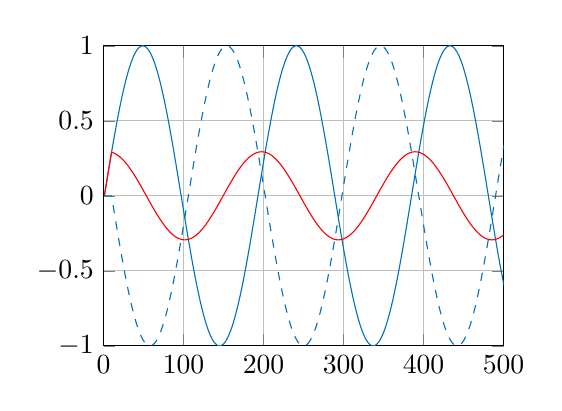
\begin{tikzpicture}

\begin{axis}[%
width=2in,
height=1.5in,
scale only axis,
xmin=0,
xmax=500,
xmajorgrids,
ymin=-1,
ymax=1,
ymajorgrids,
axis background/.style={fill=white}
]
\addplot [color=mycolor1,solid,forget plot]
  table[row sep=crcr]{%
1	0\\
2	0.0327190828217761\\
3	0.0654031292301431\\
4	0.0980171403295606\\
5	0.130526192220052\\
6	0.162895473394589\\
7	0.195090322016128\\
8	0.227076263034373\\
9	0.258819045102521\\
10	0.290284677254462\\
11	0.321439465303162\\
12	0.352250047921233\\
13	0.38268343236509\\
14	0.412707029804395\\
15	0.442288690219001\\
16	0.471396736825998\\
17	0.5\\
18	0.528067850650368\\
19	0.555570233019602\\
20	0.582477696867802\\
21	0.608761429008721\\
22	0.634393284163645\\
23	0.659345815100069\\
24	0.683592302022871\\
25	0.707106781186547\\
26	0.729864072697836\\
27	0.751839807478977\\
28	0.773010453362737\\
29	0.793353340291235\\
30	0.812846684591615\\
31	0.831469612302545\\
32	0.849202181526579\\
33	0.866025403784439\\
34	0.881921264348355\\
35	0.896872741532688\\
36	0.910863824921176\\
37	0.923879532511287\\
38	0.935905926757326\\
39	0.946930129495106\\
40	0.956940335732209\\
41	0.965925826289068\\
42	0.973876979277334\\
43	0.98078528040323\\
44	0.986643332084879\\
45	0.99144486137381\\
46	0.995184726672197\\
47	0.997858923238603\\
48	0.999464587476366\\
49	1\\
50	0.999464587476366\\
51	0.997858923238603\\
52	0.995184726672197\\
53	0.99144486137381\\
54	0.986643332084879\\
55	0.980785280403231\\
56	0.973876979277334\\
57	0.965925826289068\\
58	0.956940335732209\\
59	0.946930129495106\\
60	0.935905926757326\\
61	0.923879532511287\\
62	0.910863824921176\\
63	0.896872741532688\\
64	0.881921264348355\\
65	0.866025403784439\\
66	0.849202181526579\\
67	0.831469612302545\\
68	0.812846684591615\\
69	0.793353340291235\\
70	0.773010453362737\\
71	0.751839807478978\\
72	0.729864072697836\\
73	0.707106781186548\\
74	0.683592302022872\\
75	0.659345815100069\\
76	0.634393284163645\\
77	0.60876142900872\\
78	0.582477696867802\\
79	0.555570233019603\\
80	0.528067850650368\\
81	0.5\\
82	0.471396736825998\\
83	0.442288690219002\\
84	0.412707029804395\\
85	0.38268343236509\\
86	0.352250047921233\\
87	0.321439465303161\\
88	0.290284677254463\\
89	0.258819045102521\\
90	0.227076263034374\\
91	0.195090322016129\\
92	0.162895473394589\\
93	0.130526192220052\\
94	0.0980171403295608\\
95	0.0654031292301431\\
96	0.0327190828217764\\
97	1.22464679914735e-16\\
98	-0.0327190828217758\\
99	-0.0654031292301424\\
100	-0.0980171403295606\\
101	-0.130526192220051\\
102	-0.162895473394588\\
103	-0.195090322016128\\
104	-0.227076263034373\\
105	-0.258819045102521\\
106	-0.290284677254462\\
107	-0.321439465303162\\
108	-0.352250047921233\\
109	-0.382683432365089\\
110	-0.412707029804395\\
111	-0.442288690219001\\
112	-0.471396736825998\\
113	-0.5\\
114	-0.528067850650368\\
115	-0.555570233019602\\
116	-0.582477696867802\\
117	-0.608761429008721\\
118	-0.634393284163645\\
119	-0.659345815100069\\
120	-0.683592302022871\\
121	-0.707106781186548\\
122	-0.729864072697836\\
123	-0.751839807478977\\
124	-0.773010453362737\\
125	-0.793353340291235\\
126	-0.812846684591615\\
127	-0.831469612302545\\
128	-0.849202181526579\\
129	-0.866025403784438\\
130	-0.881921264348354\\
131	-0.896872741532688\\
132	-0.910863824921175\\
133	-0.923879532511287\\
134	-0.935905926757326\\
135	-0.946930129495106\\
136	-0.956940335732209\\
137	-0.965925826289068\\
138	-0.973876979277334\\
139	-0.98078528040323\\
140	-0.986643332084879\\
141	-0.99144486137381\\
142	-0.995184726672197\\
143	-0.997858923238603\\
144	-0.999464587476366\\
145	-1\\
146	-0.999464587476366\\
147	-0.997858923238604\\
148	-0.995184726672197\\
149	-0.99144486137381\\
150	-0.986643332084879\\
151	-0.98078528040323\\
152	-0.973876979277334\\
153	-0.965925826289068\\
154	-0.956940335732209\\
155	-0.946930129495105\\
156	-0.935905926757326\\
157	-0.923879532511287\\
158	-0.910863824921176\\
159	-0.896872741532688\\
160	-0.881921264348355\\
161	-0.866025403784439\\
162	-0.849202181526579\\
163	-0.831469612302545\\
164	-0.812846684591615\\
165	-0.793353340291236\\
166	-0.773010453362737\\
167	-0.751839807478978\\
168	-0.729864072697836\\
169	-0.707106781186548\\
170	-0.683592302022872\\
171	-0.659345815100069\\
172	-0.634393284163646\\
173	-0.60876142900872\\
174	-0.582477696867802\\
175	-0.555570233019603\\
176	-0.528067850650368\\
177	-0.5\\
178	-0.471396736825998\\
179	-0.442288690219002\\
180	-0.412707029804395\\
181	-0.38268343236509\\
182	-0.352250047921234\\
183	-0.321439465303162\\
184	-0.290284677254463\\
185	-0.258819045102522\\
186	-0.227076263034374\\
187	-0.195090322016129\\
188	-0.162895473394589\\
189	-0.130526192220052\\
190	-0.0980171403295605\\
191	-0.0654031292301437\\
192	-0.0327190828217766\\
193	-2.44929359829471e-16\\
194	0.0327190828217752\\
195	0.0654031292301423\\
196	0.0980171403295609\\
197	0.13052619222005\\
198	0.162895473394589\\
199	0.195090322016128\\
200	0.227076263034373\\
201	0.25881904510252\\
202	0.290284677254462\\
203	0.321439465303161\\
204	0.352250047921233\\
205	0.382683432365089\\
206	0.412707029804394\\
207	0.442288690219002\\
208	0.471396736825997\\
209	0.5\\
210	0.528067850650368\\
211	0.555570233019601\\
212	0.582477696867802\\
213	0.608761429008721\\
214	0.634393284163645\\
215	0.659345815100068\\
216	0.683592302022872\\
217	0.707106781186547\\
218	0.729864072697836\\
219	0.751839807478978\\
220	0.773010453362736\\
221	0.793353340291235\\
222	0.812846684591615\\
223	0.831469612302545\\
224	0.849202181526578\\
225	0.866025403784438\\
226	0.881921264348355\\
227	0.896872741532689\\
228	0.910863824921175\\
229	0.923879532511287\\
230	0.935905926757326\\
231	0.946930129495105\\
232	0.956940335732209\\
233	0.965925826289068\\
234	0.973876979277334\\
235	0.98078528040323\\
236	0.986643332084879\\
237	0.99144486137381\\
238	0.995184726672197\\
239	0.997858923238603\\
240	0.999464587476366\\
241	1\\
242	0.999464587476366\\
243	0.997858923238603\\
244	0.995184726672197\\
245	0.99144486137381\\
246	0.986643332084879\\
247	0.98078528040323\\
248	0.973876979277334\\
249	0.965925826289068\\
250	0.956940335732209\\
251	0.946930129495106\\
252	0.935905926757325\\
253	0.923879532511287\\
254	0.910863824921176\\
255	0.896872741532688\\
256	0.881921264348355\\
257	0.866025403784439\\
258	0.849202181526579\\
259	0.831469612302547\\
260	0.812846684591615\\
261	0.793353340291235\\
262	0.773010453362738\\
263	0.751839807478978\\
264	0.729864072697835\\
265	0.707106781186548\\
266	0.683592302022871\\
267	0.65934581510007\\
268	0.634393284163647\\
269	0.608761429008721\\
270	0.582477696867803\\
271	0.555570233019602\\
272	0.528067850650369\\
273	0.5\\
274	0.471396736825998\\
275	0.442288690219001\\
276	0.412707029804396\\
277	0.382683432365091\\
278	0.352250047921233\\
279	0.321439465303162\\
280	0.290284677254463\\
281	0.258819045102523\\
282	0.227076263034374\\
283	0.195090322016128\\
284	0.162895473394589\\
285	0.130526192220053\\
286	0.0980171403295624\\
287	0.0654031292301438\\
288	0.0327190828217758\\
289	3.67394039744206e-16\\
290	-0.0327190828217751\\
291	-0.0654031292301431\\
292	-0.0980171403295617\\
293	-0.13052619222005\\
294	-0.162895473394588\\
295	-0.195090322016126\\
296	-0.227076263034373\\
297	-0.25881904510252\\
298	-0.290284677254461\\
299	-0.32143946530316\\
300	-0.352250047921234\\
301	-0.38268343236509\\
302	-0.412707029804394\\
303	-0.442288690219\\
304	-0.471396736825996\\
305	-0.500000000000001\\
306	-0.528067850650368\\
307	-0.555570233019602\\
308	-0.582477696867801\\
309	-0.608761429008722\\
310	-0.634393284163645\\
311	-0.659345815100069\\
312	-0.68359230202287\\
313	-0.707106781186547\\
314	-0.729864072697835\\
315	-0.751839807478977\\
316	-0.773010453362736\\
317	-0.793353340291235\\
318	-0.812846684591614\\
319	-0.831469612302545\\
320	-0.849202181526578\\
321	-0.866025403784438\\
322	-0.881921264348355\\
323	-0.896872741532689\\
324	-0.910863824921176\\
325	-0.923879532511286\\
326	-0.935905926757325\\
327	-0.946930129495105\\
328	-0.956940335732209\\
329	-0.965925826289068\\
330	-0.973876979277333\\
331	-0.98078528040323\\
332	-0.986643332084879\\
333	-0.99144486137381\\
334	-0.995184726672197\\
335	-0.997858923238603\\
336	-0.999464587476366\\
337	-1\\
338	-0.999464587476366\\
339	-0.997858923238604\\
340	-0.995184726672197\\
341	-0.99144486137381\\
342	-0.986643332084879\\
343	-0.980785280403231\\
344	-0.973876979277334\\
345	-0.965925826289068\\
346	-0.956940335732209\\
347	-0.946930129495106\\
348	-0.935905926757326\\
349	-0.923879532511287\\
350	-0.910863824921176\\
351	-0.896872741532688\\
352	-0.881921264348356\\
353	-0.866025403784439\\
354	-0.849202181526579\\
355	-0.831469612302546\\
356	-0.812846684591616\\
357	-0.793353340291236\\
358	-0.773010453362738\\
359	-0.751839807478977\\
360	-0.729864072697836\\
361	-0.707106781186548\\
362	-0.683592302022871\\
363	-0.65934581510007\\
364	-0.634393284163645\\
365	-0.608761429008721\\
366	-0.582477696867803\\
367	-0.555570233019604\\
368	-0.528067850650367\\
369	-0.500000000000001\\
370	-0.471396736825998\\
371	-0.442288690219002\\
372	-0.412707029804395\\
373	-0.382683432365091\\
374	-0.352250047921235\\
375	-0.321439465303162\\
376	-0.290284677254464\\
377	-0.258819045102521\\
378	-0.227076263034376\\
379	-0.195090322016128\\
380	-0.162895473394591\\
381	-0.130526192220053\\
382	-0.0980171403295608\\
383	-0.0654031292301439\\
384	-0.0327190828217795\\
385	-4.89858719658941e-16\\
386	0.032719082821775\\
387	0.0654031292301412\\
388	0.0980171403295598\\
389	0.13052619222005\\
390	0.162895473394588\\
391	0.195090322016129\\
392	0.227076263034373\\
393	0.258819045102518\\
394	0.290284677254461\\
395	0.321439465303161\\
396	0.352250047921232\\
397	0.38268343236509\\
398	0.412707029804394\\
399	0.442288690219\\
400	0.471396736825999\\
401	0.499999999999999\\
402	0.528067850650366\\
403	0.555570233019602\\
404	0.582477696867802\\
405	0.608761429008719\\
406	0.634393284163646\\
407	0.659345815100068\\
408	0.683592302022871\\
409	0.707106781186547\\
410	0.729864072697835\\
411	0.751839807478977\\
412	0.773010453362735\\
413	0.793353340291236\\
414	0.812846684591614\\
415	0.831469612302544\\
416	0.849202181526578\\
417	0.866025403784439\\
418	0.881921264348354\\
419	0.896872741532688\\
420	0.910863824921175\\
421	0.923879532511286\\
422	0.935905926757326\\
423	0.946930129495105\\
424	0.956940335732208\\
425	0.965925826289068\\
426	0.973876979277333\\
427	0.98078528040323\\
428	0.986643332084879\\
429	0.99144486137381\\
430	0.995184726672197\\
431	0.997858923238604\\
432	0.999464587476366\\
433	1\\
434	0.999464587476366\\
435	0.997858923238603\\
436	0.995184726672197\\
437	0.99144486137381\\
438	0.986643332084879\\
439	0.980785280403231\\
440	0.973876979277334\\
441	0.965925826289069\\
442	0.956940335732209\\
443	0.946930129495106\\
444	0.935905926757326\\
445	0.923879532511287\\
446	0.910863824921177\\
447	0.896872741532689\\
448	0.881921264348356\\
449	0.866025403784439\\
450	0.849202181526579\\
451	0.831469612302546\\
452	0.812846684591617\\
453	0.793353340291234\\
454	0.773010453362738\\
455	0.751839807478979\\
456	0.729864072697836\\
457	0.707106781186549\\
458	0.683592302022873\\
459	0.659345815100068\\
460	0.634393284163647\\
461	0.608761429008723\\
462	0.582477696867802\\
463	0.555570233019603\\
464	0.528067850650369\\
465	0.5\\
466	0.471396736825998\\
467	0.442288690219003\\
468	0.412707029804397\\
469	0.382683432365091\\
470	0.352250047921235\\
471	0.321439465303164\\
472	0.290284677254462\\
473	0.258819045102523\\
474	0.227076263034376\\
475	0.19509032201613\\
476	0.162895473394589\\
477	0.130526192220053\\
478	0.0980171403295609\\
479	0.0654031292301458\\
480	0.0327190828217761\\
481	-1.16403343982657e-15\\
482	-0.0327190828217784\\
483	-0.0654031292301428\\
484	-0.0980171403295579\\
485	-0.130526192220055\\
486	-0.16289547339459\\
487	-0.195090322016127\\
488	-0.227076263034373\\
489	-0.258819045102523\\
490	-0.290284677254461\\
491	-0.321439465303161\\
492	-0.352250047921237\\
493	-0.382683432365091\\
494	-0.412707029804397\\
495	-0.442288690219001\\
496	-0.471396736825999\\
497	-0.499999999999999\\
498	-0.528067850650368\\
499	-0.5555702330196\\
500	-0.582477696867804\\
501	-0.608761429008723\\
502	-0.634393284163646\\
503	-0.65934581510007\\
504	-0.683592302022873\\
505	-0.707106781186548\\
506	-0.729864072697834\\
507	-0.751839807478977\\
508	-0.773010453362737\\
509	-0.793353340291236\\
510	-0.812846684591616\\
511	-0.831469612302547\\
512	-0.849202181526579\\
513	-0.866025403784439\\
514	-0.881921264348355\\
515	-0.896872741532688\\
516	-0.910863824921176\\
517	-0.923879532511286\\
518	-0.935905926757326\\
519	-0.946930129495107\\
520	-0.956940335732209\\
521	-0.965925826289068\\
522	-0.973876979277334\\
523	-0.980785280403231\\
524	-0.986643332084879\\
525	-0.99144486137381\\
526	-0.995184726672197\\
527	-0.997858923238604\\
528	-0.999464587476366\\
529	-1\\
530	-0.999464587476366\\
531	-0.997858923238603\\
532	-0.995184726672197\\
533	-0.991444861373811\\
534	-0.986643332084879\\
535	-0.98078528040323\\
536	-0.973876979277333\\
537	-0.965925826289069\\
538	-0.956940335732208\\
539	-0.946930129495105\\
540	-0.935905926757326\\
541	-0.923879532511287\\
542	-0.910863824921175\\
543	-0.896872741532689\\
544	-0.881921264348355\\
545	-0.866025403784438\\
546	-0.849202181526578\\
547	-0.831469612302544\\
548	-0.812846684591615\\
549	-0.793353340291234\\
550	-0.773010453362736\\
551	-0.751839807478978\\
552	-0.729864072697837\\
553	-0.707106781186546\\
554	-0.683592302022869\\
555	-0.659345815100069\\
556	-0.634393284163644\\
557	-0.608761429008719\\
558	-0.582477696867802\\
559	-0.555570233019604\\
560	-0.528067850650369\\
561	-0.5\\
562	-0.471396736826\\
563	-0.442288690218999\\
564	-0.412707029804392\\
565	-0.382683432365089\\
566	-0.352250047921232\\
567	-0.321439465303162\\
568	-0.290284677254462\\
569	-0.258819045102519\\
570	-0.227076263034374\\
571	-0.195090322016132\\
572	-0.162895473394588\\
573	-0.13052619222005\\
574	-0.098017140329561\\
575	-0.0654031292301424\\
576	-0.0327190828217744\\
577	-7.34788079488412e-16\\
578	0.0327190828217765\\
579	0.0654031292301409\\
580	0.0980171403295595\\
581	0.130526192220055\\
582	0.16289547339459\\
583	0.19509032201613\\
584	0.227076263034376\\
585	0.258819045102521\\
586	0.290284677254461\\
587	0.321439465303164\\
588	0.352250047921234\\
589	0.382683432365088\\
590	0.412707029804397\\
591	0.442288690219005\\
592	0.471396736825999\\
593	0.500000000000002\\
594	0.528067850650368\\
595	0.555570233019603\\
596	0.582477696867804\\
597	0.608761429008717\\
598	0.634393284163646\\
599	0.65934581510007\\
600	0.683592302022871\\
601	0.707106781186548\\
602	0.729864072697836\\
603	0.751839807478977\\
604	0.773010453362737\\
605	0.793353340291236\\
606	0.812846684591614\\
607	0.831469612302545\\
608	0.849202181526579\\
609	0.866025403784439\\
610	0.881921264348356\\
611	0.896872741532688\\
612	0.910863824921175\\
613	0.923879532511286\\
614	0.935905926757326\\
615	0.946930129495105\\
616	0.956940335732208\\
617	0.965925826289069\\
618	0.973876979277334\\
619	0.980785280403231\\
620	0.986643332084879\\
621	0.99144486137381\\
622	0.995184726672197\\
623	0.997858923238603\\
624	0.999464587476366\\
625	1\\
626	0.999464587476366\\
627	0.997858923238604\\
628	0.995184726672197\\
629	0.99144486137381\\
630	0.986643332084879\\
631	0.98078528040323\\
632	0.973876979277334\\
633	0.965925826289069\\
634	0.956940335732209\\
635	0.946930129495105\\
636	0.935905926757325\\
637	0.923879532511286\\
638	0.910863824921176\\
639	0.896872741532689\\
640	0.881921264348354\\
641	0.866025403784438\\
642	0.84920218152658\\
643	0.831469612302546\\
644	0.812846684591613\\
645	0.793353340291235\\
646	0.773010453362736\\
647	0.751839807478978\\
648	0.729864072697835\\
649	0.707106781186546\\
650	0.683592302022872\\
651	0.659345815100069\\
652	0.634393284163644\\
653	0.608761429008721\\
654	0.582477696867802\\
655	0.555570233019601\\
656	0.528067850650369\\
657	0.5\\
658	0.471396736825997\\
659	0.442288690219003\\
660	0.412707029804395\\
661	0.382683432365089\\
662	0.352250047921232\\
663	0.321439465303159\\
664	0.290284677254459\\
665	0.258819045102523\\
666	0.227076263034374\\
667	0.195090322016125\\
668	0.162895473394591\\
669	0.130526192220053\\
670	0.0980171403295611\\
671	0.0654031292301425\\
672	0.0327190828217745\\
673	8.57252759403147e-16\\
674	-0.0327190828217764\\
675	-0.0654031292301444\\
676	-0.0980171403295594\\
677	-0.130526192220048\\
678	-0.16289547339459\\
679	-0.195090322016127\\
680	-0.227076263034373\\
681	-0.258819045102521\\
682	-0.290284677254464\\
683	-0.321439465303161\\
684	-0.352250047921234\\
685	-0.382683432365091\\
686	-0.412707029804394\\
687	-0.442288690219001\\
688	-0.471396736825995\\
689	-0.500000000000002\\
690	-0.528067850650371\\
691	-0.555570233019603\\
692	-0.582477696867801\\
693	-0.608761429008723\\
694	-0.634393284163646\\
695	-0.659345815100067\\
696	-0.68359230202287\\
697	-0.707106781186548\\
698	-0.729864072697836\\
699	-0.751839807478979\\
700	-0.773010453362737\\
701	-0.793353340291236\\
702	-0.812846684591616\\
703	-0.831469612302545\\
704	-0.849202181526579\\
705	-0.866025403784439\\
706	-0.881921264348355\\
707	-0.896872741532688\\
708	-0.910863824921176\\
709	-0.923879532511288\\
710	-0.935905926757326\\
711	-0.946930129495106\\
712	-0.956940335732209\\
713	-0.965925826289068\\
714	-0.973876979277334\\
715	-0.98078528040323\\
716	-0.986643332084879\\
717	-0.991444861373811\\
718	-0.995184726672197\\
719	-0.997858923238603\\
720	-0.999464587476366\\
721	-1\\
722	-0.999464587476366\\
723	-0.997858923238604\\
724	-0.995184726672197\\
725	-0.99144486137381\\
726	-0.986643332084879\\
727	-0.98078528040323\\
728	-0.973876979277333\\
729	-0.965925826289069\\
730	-0.956940335732209\\
731	-0.946930129495105\\
732	-0.935905926757326\\
733	-0.923879532511288\\
734	-0.910863824921176\\
735	-0.896872741532688\\
736	-0.881921264348355\\
737	-0.866025403784438\\
738	-0.849202181526578\\
739	-0.831469612302546\\
740	-0.812846684591615\\
741	-0.793353340291237\\
742	-0.773010453362738\\
743	-0.751839807478975\\
744	-0.729864072697835\\
745	-0.707106781186549\\
746	-0.683592302022869\\
747	-0.659345815100069\\
748	-0.634393284163647\\
749	-0.608761429008722\\
750	-0.582477696867802\\
751	-0.555570233019604\\
752	-0.528067850650366\\
753	-0.499999999999997\\
754	-0.471396736825997\\
755	-0.442288690219\\
756	-0.412707029804392\\
757	-0.382683432365089\\
758	-0.352250047921232\\
759	-0.321439465303159\\
760	-0.290284677254466\\
761	-0.25881904510252\\
762	-0.227076263034368\\
763	-0.195090322016129\\
764	-0.162895473394588\\
765	-0.13052619222005\\
766	-0.0980171403295612\\
767	-0.0654031292301426\\
768	-0.0327190828217746\\
769	-9.79717439317883e-16\\
770	0.0327190828217798\\
771	0.0654031292301478\\
772	0.0980171403295593\\
773	0.130526192220055\\
774	0.162895473394586\\
775	0.195090322016127\\
776	0.227076263034373\\
777	0.258819045102518\\
778	0.29028467725446\\
779	0.321439465303164\\
780	0.352250047921234\\
781	0.382683432365091\\
782	0.412707029804397\\
783	0.442288690219001\\
784	0.471396736825998\\
785	0.500000000000002\\
786	0.528067850650365\\
787	0.5555702330196\\
788	0.582477696867806\\
789	0.60876142900872\\
790	0.634393284163646\\
791	0.65934581510007\\
792	0.68359230202287\\
793	0.707106781186547\\
794	0.729864072697836\\
795	0.751839807478976\\
796	0.773010453362737\\
797	0.793353340291238\\
798	0.812846684591614\\
799	0.831469612302547\\
800	0.849202181526577\\
801	0.866025403784437\\
802	0.881921264348354\\
803	0.896872741532687\\
804	0.910863824921175\\
805	0.923879532511286\\
806	0.935905926757326\\
807	0.946930129495106\\
808	0.956940335732209\\
809	0.965925826289067\\
810	0.973876979277334\\
811	0.980785280403231\\
812	0.986643332084878\\
813	0.99144486137381\\
814	0.995184726672197\\
815	0.997858923238603\\
816	0.999464587476366\\
817	1\\
818	0.999464587476366\\
819	0.997858923238604\\
820	0.995184726672197\\
821	0.991444861373811\\
822	0.986643332084879\\
823	0.98078528040323\\
824	0.973876979277334\\
825	0.965925826289068\\
826	0.956940335732208\\
827	0.946930129495107\\
828	0.935905926757326\\
829	0.923879532511287\\
830	0.910863824921177\\
831	0.896872741532689\\
832	0.881921264348355\\
833	0.866025403784439\\
834	0.849202181526578\\
835	0.831469612302544\\
836	0.812846684591615\\
837	0.793353340291235\\
838	0.773010453362736\\
839	0.75183980747898\\
840	0.729864072697838\\
841	0.707106781186546\\
842	0.683592302022872\\
843	0.659345815100069\\
844	0.634393284163644\\
845	0.608761429008722\\
846	0.582477696867802\\
847	0.555570233019602\\
848	0.528067850650369\\
849	0.5\\
850	0.471396736825997\\
851	0.442288690219003\\
852	0.412707029804392\\
853	0.382683432365086\\
854	0.352250047921236\\
855	0.321439465303163\\
856	0.290284677254462\\
857	0.258819045102523\\
858	0.227076263034375\\
859	0.195090322016129\\
860	0.162895473394588\\
861	0.13052619222005\\
862	0.0980171403295578\\
863	0.0654031292301428\\
864	0.0327190828217748\\
865	-2.45053155956788e-15\\
866	-0.0327190828217726\\
867	-0.0654031292301441\\
868	-0.0980171403295627\\
869	-0.130526192220051\\
870	-0.162895473394589\\
871	-0.19509032201613\\
872	-0.227076263034373\\
873	-0.258819045102521\\
874	-0.290284677254464\\
875	-0.321439465303161\\
876	-0.352250047921234\\
877	-0.382683432365084\\
878	-0.412707029804397\\
879	-0.442288690219004\\
880	-0.471396736825995\\
881	-0.499999999999999\\
882	-0.528067850650367\\
883	-0.5555702330196\\
884	-0.5824776968678\\
885	-0.60876142900872\\
886	-0.634393284163643\\
887	-0.65934581510007\\
888	-0.683592302022873\\
889	-0.707106781186547\\
890	-0.729864072697836\\
891	-0.751839807478979\\
892	-0.773010453362734\\
893	-0.793353340291233\\
894	-0.812846684591616\\
895	-0.831469612302543\\
896	-0.849202181526579\\
897	-0.866025403784439\\
898	-0.881921264348354\\
899	-0.896872741532688\\
900	-0.910863824921176\\
901	-0.923879532511286\\
902	-0.935905926757326\\
903	-0.946930129495106\\
904	-0.956940335732207\\
905	-0.965925826289069\\
906	-0.973876979277335\\
907	-0.98078528040323\\
908	-0.986643332084879\\
909	-0.99144486137381\\
910	-0.995184726672197\\
911	-0.997858923238603\\
912	-0.999464587476366\\
913	-1\\
914	-0.999464587476366\\
915	-0.997858923238603\\
916	-0.995184726672197\\
917	-0.99144486137381\\
918	-0.986643332084879\\
919	-0.980785280403231\\
920	-0.973876979277333\\
921	-0.965925826289068\\
922	-0.95694033573221\\
923	-0.946930129495105\\
924	-0.935905926757325\\
925	-0.923879532511287\\
926	-0.910863824921176\\
927	-0.896872741532688\\
928	-0.881921264348355\\
929	-0.866025403784439\\
930	-0.849202181526582\\
931	-0.831469612302546\\
932	-0.812846684591613\\
933	-0.793353340291237\\
934	-0.773010453362738\\
935	-0.751839807478978\\
936	-0.729864072697838\\
937	-0.707106781186549\\
938	-0.683592302022872\\
939	-0.659345815100072\\
940	-0.634393284163647\\
941	-0.608761429008719\\
942	-0.582477696867802\\
943	-0.555570233019602\\
944	-0.528067850650366\\
945	-0.500000000000004\\
946	-0.471396736826\\
947	-0.442288690219\\
948	-0.412707029804399\\
949	-0.382683432365093\\
950	-0.352250047921232\\
951	-0.321439465303163\\
952	-0.290284677254463\\
953	-0.25881904510252\\
954	-0.227076263034375\\
955	-0.195090322016129\\
956	-0.162895473394592\\
957	-0.130526192220057\\
958	-0.0980171403295615\\
959	-0.0654031292301429\\
960	-0.0327190828217784\\
961	2.32806687965315e-15\\
};
\addplot [color=mycolor1,dashed,forget plot]
  table[row sep=crcr]{%
1	0\\
2	0\\
3	0\\
4	0\\
5	0\\
6	0\\
7	0\\
8	0\\
9	0\\
10	0\\
11	-0.0327190828217761\\
12	-0.0654031292301431\\
13	-0.0980171403295606\\
14	-0.130526192220052\\
15	-0.162895473394589\\
16	-0.195090322016128\\
17	-0.227076263034373\\
18	-0.258819045102521\\
19	-0.290284677254462\\
20	-0.321439465303162\\
21	-0.352250047921233\\
22	-0.38268343236509\\
23	-0.412707029804395\\
24	-0.442288690219001\\
25	-0.471396736825998\\
26	-0.5\\
27	-0.528067850650368\\
28	-0.555570233019602\\
29	-0.582477696867802\\
30	-0.608761429008721\\
31	-0.634393284163645\\
32	-0.659345815100069\\
33	-0.683592302022871\\
34	-0.707106781186547\\
35	-0.729864072697836\\
36	-0.751839807478977\\
37	-0.773010453362737\\
38	-0.793353340291235\\
39	-0.812846684591615\\
40	-0.831469612302545\\
41	-0.849202181526579\\
42	-0.866025403784439\\
43	-0.881921264348355\\
44	-0.896872741532688\\
45	-0.910863824921176\\
46	-0.923879532511287\\
47	-0.935905926757326\\
48	-0.946930129495106\\
49	-0.956940335732209\\
50	-0.965925826289068\\
51	-0.973876979277334\\
52	-0.98078528040323\\
53	-0.986643332084879\\
54	-0.99144486137381\\
55	-0.995184726672197\\
56	-0.997858923238603\\
57	-0.999464587476366\\
58	-1\\
59	-0.999464587476366\\
60	-0.997858923238603\\
61	-0.995184726672197\\
62	-0.99144486137381\\
63	-0.986643332084879\\
64	-0.980785280403231\\
65	-0.973876979277334\\
66	-0.965925826289068\\
67	-0.956940335732209\\
68	-0.946930129495106\\
69	-0.935905926757326\\
70	-0.923879532511287\\
71	-0.910863824921176\\
72	-0.896872741532688\\
73	-0.881921264348355\\
74	-0.866025403784439\\
75	-0.849202181526579\\
76	-0.831469612302545\\
77	-0.812846684591615\\
78	-0.793353340291235\\
79	-0.773010453362737\\
80	-0.751839807478978\\
81	-0.729864072697836\\
82	-0.707106781186548\\
83	-0.683592302022872\\
84	-0.659345815100069\\
85	-0.634393284163645\\
86	-0.60876142900872\\
87	-0.582477696867802\\
88	-0.555570233019603\\
89	-0.528067850650368\\
90	-0.5\\
91	-0.471396736825998\\
92	-0.442288690219002\\
93	-0.412707029804395\\
94	-0.38268343236509\\
95	-0.352250047921233\\
96	-0.321439465303161\\
97	-0.290284677254463\\
98	-0.258819045102521\\
99	-0.227076263034374\\
100	-0.195090322016129\\
101	-0.162895473394589\\
102	-0.130526192220052\\
103	-0.0980171403295608\\
104	-0.0654031292301431\\
105	-0.0327190828217764\\
106	-1.22464679914735e-16\\
107	0.0327190828217758\\
108	0.0654031292301424\\
109	0.0980171403295606\\
110	0.130526192220051\\
111	0.162895473394588\\
112	0.195090322016128\\
113	0.227076263034373\\
114	0.258819045102521\\
115	0.290284677254462\\
116	0.321439465303162\\
117	0.352250047921233\\
118	0.382683432365089\\
119	0.412707029804395\\
120	0.442288690219001\\
121	0.471396736825998\\
122	0.5\\
123	0.528067850650368\\
124	0.555570233019602\\
125	0.582477696867802\\
126	0.608761429008721\\
127	0.634393284163645\\
128	0.659345815100069\\
129	0.683592302022871\\
130	0.707106781186548\\
131	0.729864072697836\\
132	0.751839807478977\\
133	0.773010453362737\\
134	0.793353340291235\\
135	0.812846684591615\\
136	0.831469612302545\\
137	0.849202181526579\\
138	0.866025403784438\\
139	0.881921264348354\\
140	0.896872741532688\\
141	0.910863824921175\\
142	0.923879532511287\\
143	0.935905926757326\\
144	0.946930129495106\\
145	0.956940335732209\\
146	0.965925826289068\\
147	0.973876979277334\\
148	0.98078528040323\\
149	0.986643332084879\\
150	0.99144486137381\\
151	0.995184726672197\\
152	0.997858923238603\\
153	0.999464587476366\\
154	1\\
155	0.999464587476366\\
156	0.997858923238604\\
157	0.995184726672197\\
158	0.99144486137381\\
159	0.986643332084879\\
160	0.98078528040323\\
161	0.973876979277334\\
162	0.965925826289068\\
163	0.956940335732209\\
164	0.946930129495105\\
165	0.935905926757326\\
166	0.923879532511287\\
167	0.910863824921176\\
168	0.896872741532688\\
169	0.881921264348355\\
170	0.866025403784439\\
171	0.849202181526579\\
172	0.831469612302545\\
173	0.812846684591615\\
174	0.793353340291236\\
175	0.773010453362737\\
176	0.751839807478978\\
177	0.729864072697836\\
178	0.707106781186548\\
179	0.683592302022872\\
180	0.659345815100069\\
181	0.634393284163646\\
182	0.60876142900872\\
183	0.582477696867802\\
184	0.555570233019603\\
185	0.528067850650368\\
186	0.5\\
187	0.471396736825998\\
188	0.442288690219002\\
189	0.412707029804395\\
190	0.38268343236509\\
191	0.352250047921234\\
192	0.321439465303162\\
193	0.290284677254463\\
194	0.258819045102522\\
195	0.227076263034374\\
196	0.195090322016129\\
197	0.162895473394589\\
198	0.130526192220052\\
199	0.0980171403295605\\
200	0.0654031292301437\\
201	0.0327190828217766\\
202	2.44929359829471e-16\\
203	-0.0327190828217752\\
204	-0.0654031292301423\\
205	-0.0980171403295609\\
206	-0.13052619222005\\
207	-0.162895473394589\\
208	-0.195090322016128\\
209	-0.227076263034373\\
210	-0.25881904510252\\
211	-0.290284677254462\\
212	-0.321439465303161\\
213	-0.352250047921233\\
214	-0.382683432365089\\
215	-0.412707029804394\\
216	-0.442288690219002\\
217	-0.471396736825997\\
218	-0.5\\
219	-0.528067850650368\\
220	-0.555570233019601\\
221	-0.582477696867802\\
222	-0.608761429008721\\
223	-0.634393284163645\\
224	-0.659345815100068\\
225	-0.683592302022872\\
226	-0.707106781186547\\
227	-0.729864072697836\\
228	-0.751839807478978\\
229	-0.773010453362736\\
230	-0.793353340291235\\
231	-0.812846684591615\\
232	-0.831469612302545\\
233	-0.849202181526578\\
234	-0.866025403784438\\
235	-0.881921264348355\\
236	-0.896872741532689\\
237	-0.910863824921175\\
238	-0.923879532511287\\
239	-0.935905926757326\\
240	-0.946930129495105\\
241	-0.956940335732209\\
242	-0.965925826289068\\
243	-0.973876979277334\\
244	-0.98078528040323\\
245	-0.986643332084879\\
246	-0.99144486137381\\
247	-0.995184726672197\\
248	-0.997858923238603\\
249	-0.999464587476366\\
250	-1\\
251	-0.999464587476366\\
252	-0.997858923238603\\
253	-0.995184726672197\\
254	-0.99144486137381\\
255	-0.986643332084879\\
256	-0.98078528040323\\
257	-0.973876979277334\\
258	-0.965925826289068\\
259	-0.956940335732209\\
260	-0.946930129495106\\
261	-0.935905926757325\\
262	-0.923879532511287\\
263	-0.910863824921176\\
264	-0.896872741532688\\
265	-0.881921264348355\\
266	-0.866025403784439\\
267	-0.849202181526579\\
268	-0.831469612302547\\
269	-0.812846684591615\\
270	-0.793353340291235\\
271	-0.773010453362738\\
272	-0.751839807478978\\
273	-0.729864072697835\\
274	-0.707106781186548\\
275	-0.683592302022871\\
276	-0.65934581510007\\
277	-0.634393284163647\\
278	-0.608761429008721\\
279	-0.582477696867803\\
280	-0.555570233019602\\
281	-0.528067850650369\\
282	-0.5\\
283	-0.471396736825998\\
284	-0.442288690219001\\
285	-0.412707029804396\\
286	-0.382683432365091\\
287	-0.352250047921233\\
288	-0.321439465303162\\
289	-0.290284677254463\\
290	-0.258819045102523\\
291	-0.227076263034374\\
292	-0.195090322016128\\
293	-0.162895473394589\\
294	-0.130526192220053\\
295	-0.0980171403295624\\
296	-0.0654031292301438\\
297	-0.0327190828217758\\
298	-3.67394039744206e-16\\
299	0.0327190828217751\\
300	0.0654031292301431\\
301	0.0980171403295617\\
302	0.13052619222005\\
303	0.162895473394588\\
304	0.195090322016126\\
305	0.227076263034373\\
306	0.25881904510252\\
307	0.290284677254461\\
308	0.32143946530316\\
309	0.352250047921234\\
310	0.38268343236509\\
311	0.412707029804394\\
312	0.442288690219\\
313	0.471396736825996\\
314	0.500000000000001\\
315	0.528067850650368\\
316	0.555570233019602\\
317	0.582477696867801\\
318	0.608761429008722\\
319	0.634393284163645\\
320	0.659345815100069\\
321	0.68359230202287\\
322	0.707106781186547\\
323	0.729864072697835\\
324	0.751839807478977\\
325	0.773010453362736\\
326	0.793353340291235\\
327	0.812846684591614\\
328	0.831469612302545\\
329	0.849202181526578\\
330	0.866025403784438\\
331	0.881921264348355\\
332	0.896872741532689\\
333	0.910863824921176\\
334	0.923879532511286\\
335	0.935905926757325\\
336	0.946930129495105\\
337	0.956940335732209\\
338	0.965925826289068\\
339	0.973876979277333\\
340	0.98078528040323\\
341	0.986643332084879\\
342	0.99144486137381\\
343	0.995184726672197\\
344	0.997858923238603\\
345	0.999464587476366\\
346	1\\
347	0.999464587476366\\
348	0.997858923238604\\
349	0.995184726672197\\
350	0.99144486137381\\
351	0.986643332084879\\
352	0.980785280403231\\
353	0.973876979277334\\
354	0.965925826289068\\
355	0.956940335732209\\
356	0.946930129495106\\
357	0.935905926757326\\
358	0.923879532511287\\
359	0.910863824921176\\
360	0.896872741532688\\
361	0.881921264348356\\
362	0.866025403784439\\
363	0.849202181526579\\
364	0.831469612302546\\
365	0.812846684591616\\
366	0.793353340291236\\
367	0.773010453362738\\
368	0.751839807478977\\
369	0.729864072697836\\
370	0.707106781186548\\
371	0.683592302022871\\
372	0.65934581510007\\
373	0.634393284163645\\
374	0.608761429008721\\
375	0.582477696867803\\
376	0.555570233019604\\
377	0.528067850650367\\
378	0.500000000000001\\
379	0.471396736825998\\
380	0.442288690219002\\
381	0.412707029804395\\
382	0.382683432365091\\
383	0.352250047921235\\
384	0.321439465303162\\
385	0.290284677254464\\
386	0.258819045102521\\
387	0.227076263034376\\
388	0.195090322016128\\
389	0.162895473394591\\
390	0.130526192220053\\
391	0.0980171403295608\\
392	0.0654031292301439\\
393	0.0327190828217795\\
394	4.89858719658941e-16\\
395	-0.032719082821775\\
396	-0.0654031292301412\\
397	-0.0980171403295598\\
398	-0.13052619222005\\
399	-0.162895473394588\\
400	-0.195090322016129\\
401	-0.227076263034373\\
402	-0.258819045102518\\
403	-0.290284677254461\\
404	-0.321439465303161\\
405	-0.352250047921232\\
406	-0.38268343236509\\
407	-0.412707029804394\\
408	-0.442288690219\\
409	-0.471396736825999\\
410	-0.499999999999999\\
411	-0.528067850650366\\
412	-0.555570233019602\\
413	-0.582477696867802\\
414	-0.608761429008719\\
415	-0.634393284163646\\
416	-0.659345815100068\\
417	-0.683592302022871\\
418	-0.707106781186547\\
419	-0.729864072697835\\
420	-0.751839807478977\\
421	-0.773010453362735\\
422	-0.793353340291236\\
423	-0.812846684591614\\
424	-0.831469612302544\\
425	-0.849202181526578\\
426	-0.866025403784439\\
427	-0.881921264348354\\
428	-0.896872741532688\\
429	-0.910863824921175\\
430	-0.923879532511286\\
431	-0.935905926757326\\
432	-0.946930129495105\\
433	-0.956940335732208\\
434	-0.965925826289068\\
435	-0.973876979277333\\
436	-0.98078528040323\\
437	-0.986643332084879\\
438	-0.99144486137381\\
439	-0.995184726672197\\
440	-0.997858923238604\\
441	-0.999464587476366\\
442	-1\\
443	-0.999464587476366\\
444	-0.997858923238603\\
445	-0.995184726672197\\
446	-0.99144486137381\\
447	-0.986643332084879\\
448	-0.980785280403231\\
449	-0.973876979277334\\
450	-0.965925826289069\\
451	-0.956940335732209\\
452	-0.946930129495106\\
453	-0.935905926757326\\
454	-0.923879532511287\\
455	-0.910863824921177\\
456	-0.896872741532689\\
457	-0.881921264348356\\
458	-0.866025403784439\\
459	-0.849202181526579\\
460	-0.831469612302546\\
461	-0.812846684591617\\
462	-0.793353340291234\\
463	-0.773010453362738\\
464	-0.751839807478979\\
465	-0.729864072697836\\
466	-0.707106781186549\\
467	-0.683592302022873\\
468	-0.659345815100068\\
469	-0.634393284163647\\
470	-0.608761429008723\\
471	-0.582477696867802\\
472	-0.555570233019603\\
473	-0.528067850650369\\
474	-0.5\\
475	-0.471396736825998\\
476	-0.442288690219003\\
477	-0.412707029804397\\
478	-0.382683432365091\\
479	-0.352250047921235\\
480	-0.321439465303164\\
481	-0.290284677254462\\
482	-0.258819045102523\\
483	-0.227076263034376\\
484	-0.19509032201613\\
485	-0.162895473394589\\
486	-0.130526192220053\\
487	-0.0980171403295609\\
488	-0.0654031292301458\\
489	-0.0327190828217761\\
490	1.16403343982657e-15\\
491	0.0327190828217784\\
492	0.0654031292301428\\
493	0.0980171403295579\\
494	0.130526192220055\\
495	0.16289547339459\\
496	0.195090322016127\\
497	0.227076263034373\\
498	0.258819045102523\\
499	0.290284677254461\\
500	0.321439465303161\\
501	0.352250047921237\\
502	0.382683432365091\\
503	0.412707029804397\\
504	0.442288690219001\\
505	0.471396736825999\\
506	0.499999999999999\\
507	0.528067850650368\\
508	0.5555702330196\\
509	0.582477696867804\\
510	0.608761429008723\\
511	0.634393284163646\\
512	0.65934581510007\\
513	0.683592302022873\\
514	0.707106781186548\\
515	0.729864072697834\\
516	0.751839807478977\\
517	0.773010453362737\\
518	0.793353340291236\\
519	0.812846684591616\\
520	0.831469612302547\\
521	0.849202181526579\\
522	0.866025403784439\\
523	0.881921264348355\\
524	0.896872741532688\\
525	0.910863824921176\\
526	0.923879532511286\\
527	0.935905926757326\\
528	0.946930129495107\\
529	0.956940335732209\\
530	0.965925826289068\\
531	0.973876979277334\\
532	0.980785280403231\\
533	0.986643332084879\\
534	0.99144486137381\\
535	0.995184726672197\\
536	0.997858923238604\\
537	0.999464587476366\\
538	1\\
539	0.999464587476366\\
540	0.997858923238603\\
541	0.995184726672197\\
542	0.991444861373811\\
543	0.986643332084879\\
544	0.98078528040323\\
545	0.973876979277333\\
546	0.965925826289069\\
547	0.956940335732208\\
548	0.946930129495105\\
549	0.935905926757326\\
550	0.923879532511287\\
551	0.910863824921175\\
552	0.896872741532689\\
553	0.881921264348355\\
554	0.866025403784438\\
555	0.849202181526578\\
556	0.831469612302544\\
557	0.812846684591615\\
558	0.793353340291234\\
559	0.773010453362736\\
560	0.751839807478978\\
561	0.729864072697837\\
562	0.707106781186546\\
563	0.683592302022869\\
564	0.659345815100069\\
565	0.634393284163644\\
566	0.608761429008719\\
567	0.582477696867802\\
568	0.555570233019604\\
569	0.528067850650369\\
570	0.5\\
571	0.471396736826\\
572	0.442288690218999\\
573	0.412707029804392\\
574	0.382683432365089\\
575	0.352250047921232\\
576	0.321439465303162\\
577	0.290284677254462\\
578	0.258819045102519\\
579	0.227076263034374\\
580	0.195090322016132\\
581	0.162895473394588\\
582	0.13052619222005\\
583	0.098017140329561\\
584	0.0654031292301424\\
585	0.0327190828217744\\
586	7.34788079488412e-16\\
587	-0.0327190828217765\\
588	-0.0654031292301409\\
589	-0.0980171403295595\\
590	-0.130526192220055\\
591	-0.16289547339459\\
592	-0.19509032201613\\
593	-0.227076263034376\\
594	-0.258819045102521\\
595	-0.290284677254461\\
596	-0.321439465303164\\
597	-0.352250047921234\\
598	-0.382683432365088\\
599	-0.412707029804397\\
600	-0.442288690219005\\
601	-0.471396736825999\\
602	-0.500000000000002\\
603	-0.528067850650368\\
604	-0.555570233019603\\
605	-0.582477696867804\\
606	-0.608761429008717\\
607	-0.634393284163646\\
608	-0.65934581510007\\
609	-0.683592302022871\\
610	-0.707106781186548\\
611	-0.729864072697836\\
612	-0.751839807478977\\
613	-0.773010453362737\\
614	-0.793353340291236\\
615	-0.812846684591614\\
616	-0.831469612302545\\
617	-0.849202181526579\\
618	-0.866025403784439\\
619	-0.881921264348356\\
620	-0.896872741532688\\
621	-0.910863824921175\\
622	-0.923879532511286\\
623	-0.935905926757326\\
624	-0.946930129495105\\
625	-0.956940335732208\\
626	-0.965925826289069\\
627	-0.973876979277334\\
628	-0.980785280403231\\
629	-0.986643332084879\\
630	-0.99144486137381\\
631	-0.995184726672197\\
632	-0.997858923238603\\
633	-0.999464587476366\\
634	-1\\
635	-0.999464587476366\\
636	-0.997858923238604\\
637	-0.995184726672197\\
638	-0.99144486137381\\
639	-0.986643332084879\\
640	-0.98078528040323\\
641	-0.973876979277334\\
642	-0.965925826289069\\
643	-0.956940335732209\\
644	-0.946930129495105\\
645	-0.935905926757325\\
646	-0.923879532511286\\
647	-0.910863824921176\\
648	-0.896872741532689\\
649	-0.881921264348354\\
650	-0.866025403784438\\
651	-0.84920218152658\\
652	-0.831469612302546\\
653	-0.812846684591613\\
654	-0.793353340291235\\
655	-0.773010453362736\\
656	-0.751839807478978\\
657	-0.729864072697835\\
658	-0.707106781186546\\
659	-0.683592302022872\\
660	-0.659345815100069\\
661	-0.634393284163644\\
662	-0.608761429008721\\
663	-0.582477696867802\\
664	-0.555570233019601\\
665	-0.528067850650369\\
666	-0.5\\
667	-0.471396736825997\\
668	-0.442288690219003\\
669	-0.412707029804395\\
670	-0.382683432365089\\
671	-0.352250047921232\\
672	-0.321439465303159\\
673	-0.290284677254459\\
674	-0.258819045102523\\
675	-0.227076263034374\\
676	-0.195090322016125\\
677	-0.162895473394591\\
678	-0.130526192220053\\
679	-0.0980171403295611\\
680	-0.0654031292301425\\
681	-0.0327190828217745\\
682	-8.57252759403147e-16\\
683	0.0327190828217764\\
684	0.0654031292301444\\
685	0.0980171403295594\\
686	0.130526192220048\\
687	0.16289547339459\\
688	0.195090322016127\\
689	0.227076263034373\\
690	0.258819045102521\\
691	0.290284677254464\\
692	0.321439465303161\\
693	0.352250047921234\\
694	0.382683432365091\\
695	0.412707029804394\\
696	0.442288690219001\\
697	0.471396736825995\\
698	0.500000000000002\\
699	0.528067850650371\\
700	0.555570233019603\\
701	0.582477696867801\\
702	0.608761429008723\\
703	0.634393284163646\\
704	0.659345815100067\\
705	0.68359230202287\\
706	0.707106781186548\\
707	0.729864072697836\\
708	0.751839807478979\\
709	0.773010453362737\\
710	0.793353340291236\\
711	0.812846684591616\\
712	0.831469612302545\\
713	0.849202181526579\\
714	0.866025403784439\\
715	0.881921264348355\\
716	0.896872741532688\\
717	0.910863824921176\\
718	0.923879532511288\\
719	0.935905926757326\\
720	0.946930129495106\\
721	0.956940335732209\\
722	0.965925826289068\\
723	0.973876979277334\\
724	0.98078528040323\\
725	0.986643332084879\\
726	0.991444861373811\\
727	0.995184726672197\\
728	0.997858923238603\\
729	0.999464587476366\\
730	1\\
731	0.999464587476366\\
732	0.997858923238604\\
733	0.995184726672197\\
734	0.99144486137381\\
735	0.986643332084879\\
736	0.98078528040323\\
737	0.973876979277333\\
738	0.965925826289069\\
739	0.956940335732209\\
740	0.946930129495105\\
741	0.935905926757326\\
742	0.923879532511288\\
743	0.910863824921176\\
744	0.896872741532688\\
745	0.881921264348355\\
746	0.866025403784438\\
747	0.849202181526578\\
748	0.831469612302546\\
749	0.812846684591615\\
750	0.793353340291237\\
751	0.773010453362738\\
752	0.751839807478975\\
753	0.729864072697835\\
754	0.707106781186549\\
755	0.683592302022869\\
756	0.659345815100069\\
757	0.634393284163647\\
758	0.608761429008722\\
759	0.582477696867802\\
760	0.555570233019604\\
761	0.528067850650366\\
762	0.499999999999997\\
763	0.471396736825997\\
764	0.442288690219\\
765	0.412707029804392\\
766	0.382683432365089\\
767	0.352250047921232\\
768	0.321439465303159\\
769	0.290284677254466\\
770	0.25881904510252\\
771	0.227076263034368\\
772	0.195090322016129\\
773	0.162895473394588\\
774	0.13052619222005\\
775	0.0980171403295612\\
776	0.0654031292301426\\
777	0.0327190828217746\\
778	9.79717439317883e-16\\
779	-0.0327190828217798\\
780	-0.0654031292301478\\
781	-0.0980171403295593\\
782	-0.130526192220055\\
783	-0.162895473394586\\
784	-0.195090322016127\\
785	-0.227076263034373\\
786	-0.258819045102518\\
787	-0.29028467725446\\
788	-0.321439465303164\\
789	-0.352250047921234\\
790	-0.382683432365091\\
791	-0.412707029804397\\
792	-0.442288690219001\\
793	-0.471396736825998\\
794	-0.500000000000002\\
795	-0.528067850650365\\
796	-0.5555702330196\\
797	-0.582477696867806\\
798	-0.60876142900872\\
799	-0.634393284163646\\
800	-0.65934581510007\\
801	-0.68359230202287\\
802	-0.707106781186547\\
803	-0.729864072697836\\
804	-0.751839807478976\\
805	-0.773010453362737\\
806	-0.793353340291238\\
807	-0.812846684591614\\
808	-0.831469612302547\\
809	-0.849202181526577\\
810	-0.866025403784437\\
811	-0.881921264348354\\
812	-0.896872741532687\\
813	-0.910863824921175\\
814	-0.923879532511286\\
815	-0.935905926757326\\
816	-0.946930129495106\\
817	-0.956940335732209\\
818	-0.965925826289067\\
819	-0.973876979277334\\
820	-0.980785280403231\\
821	-0.986643332084878\\
822	-0.99144486137381\\
823	-0.995184726672197\\
824	-0.997858923238603\\
825	-0.999464587476366\\
826	-1\\
827	-0.999464587476366\\
828	-0.997858923238604\\
829	-0.995184726672197\\
830	-0.991444861373811\\
831	-0.986643332084879\\
832	-0.98078528040323\\
833	-0.973876979277334\\
834	-0.965925826289068\\
835	-0.956940335732208\\
836	-0.946930129495107\\
837	-0.935905926757326\\
838	-0.923879532511287\\
839	-0.910863824921177\\
840	-0.896872741532689\\
841	-0.881921264348355\\
842	-0.866025403784439\\
843	-0.849202181526578\\
844	-0.831469612302544\\
845	-0.812846684591615\\
846	-0.793353340291235\\
847	-0.773010453362736\\
848	-0.75183980747898\\
849	-0.729864072697838\\
850	-0.707106781186546\\
851	-0.683592302022872\\
852	-0.659345815100069\\
853	-0.634393284163644\\
854	-0.608761429008722\\
855	-0.582477696867802\\
856	-0.555570233019602\\
857	-0.528067850650369\\
858	-0.5\\
859	-0.471396736825997\\
860	-0.442288690219003\\
861	-0.412707029804392\\
862	-0.382683432365086\\
863	-0.352250047921236\\
864	-0.321439465303163\\
865	-0.290284677254462\\
866	-0.258819045102523\\
867	-0.227076263034375\\
868	-0.195090322016129\\
869	-0.162895473394588\\
870	-0.13052619222005\\
871	-0.0980171403295578\\
872	-0.0654031292301428\\
873	-0.0327190828217748\\
874	2.45053155956788e-15\\
875	0.0327190828217726\\
876	0.0654031292301441\\
877	0.0980171403295627\\
878	0.130526192220051\\
879	0.162895473394589\\
880	0.19509032201613\\
881	0.227076263034373\\
882	0.258819045102521\\
883	0.290284677254464\\
884	0.321439465303161\\
885	0.352250047921234\\
886	0.382683432365084\\
887	0.412707029804397\\
888	0.442288690219004\\
889	0.471396736825995\\
890	0.499999999999999\\
891	0.528067850650367\\
892	0.5555702330196\\
893	0.5824776968678\\
894	0.60876142900872\\
895	0.634393284163643\\
896	0.65934581510007\\
897	0.683592302022873\\
898	0.707106781186547\\
899	0.729864072697836\\
900	0.751839807478979\\
901	0.773010453362734\\
902	0.793353340291233\\
903	0.812846684591616\\
904	0.831469612302543\\
905	0.849202181526579\\
906	0.866025403784439\\
907	0.881921264348354\\
908	0.896872741532688\\
909	0.910863824921176\\
910	0.923879532511286\\
911	0.935905926757326\\
912	0.946930129495106\\
913	0.956940335732207\\
914	0.965925826289069\\
915	0.973876979277335\\
916	0.98078528040323\\
917	0.986643332084879\\
918	0.99144486137381\\
919	0.995184726672197\\
920	0.997858923238603\\
921	0.999464587476366\\
922	1\\
923	0.999464587476366\\
924	0.997858923238603\\
925	0.995184726672197\\
926	0.99144486137381\\
927	0.986643332084879\\
928	0.980785280403231\\
929	0.973876979277333\\
930	0.965925826289068\\
931	0.95694033573221\\
932	0.946930129495105\\
933	0.935905926757325\\
934	0.923879532511287\\
935	0.910863824921176\\
936	0.896872741532688\\
937	0.881921264348355\\
938	0.866025403784439\\
939	0.849202181526582\\
940	0.831469612302546\\
941	0.812846684591613\\
942	0.793353340291237\\
943	0.773010453362738\\
944	0.751839807478978\\
945	0.729864072697838\\
946	0.707106781186549\\
947	0.683592302022872\\
948	0.659345815100072\\
949	0.634393284163647\\
950	0.608761429008719\\
951	0.582477696867802\\
952	0.555570233019602\\
953	0.528067850650366\\
954	0.500000000000004\\
955	0.471396736826\\
956	0.442288690219\\
957	0.412707029804399\\
958	0.382683432365093\\
959	0.352250047921232\\
960	0.321439465303163\\
961	0.290284677254463\\
962	0.25881904510252\\
963	0.227076263034375\\
964	0.195090322016129\\
965	0.162895473394592\\
966	0.130526192220057\\
967	0.0980171403295615\\
968	0.0654031292301429\\
969	0.0327190828217784\\
970	-2.32806687965315e-15\\
};
\addplot [color=red,solid,forget plot]
  table[row sep=crcr]{%
1	0\\
2	0.0327190828217761\\
3	0.0654031292301431\\
4	0.0980171403295606\\
5	0.130526192220052\\
6	0.162895473394589\\
7	0.195090322016128\\
8	0.227076263034373\\
9	0.258819045102521\\
10	0.290284677254462\\
11	0.288720382481385\\
12	0.28684691869109\\
13	0.284666292035529\\
14	0.282180837584343\\
15	0.279393216824413\\
16	0.276306414809869\\
17	0.272923736965627\\
18	0.269248805547847\\
19	0.26528555576514\\
20	0.261038231564641\\
21	0.256511381087487\\
22	0.251709851798556\\
23	0.246638785295674\\
24	0.24130361180387\\
25	0.23571004436055\\
26	0.229864072697836\\
27	0.223771956828609\\
28	0.217440220343135\\
29	0.210875643423433\\
30	0.204085255582895\\
31	0.1970763281389\\
32	0.18985636642651\\
33	0.182433101761567\\
34	0.174814483161807\\
35	0.167008668834853\\
36	0.159024017442198\\
37	0.15086907914855\\
38	0.14255258646609\\
39	0.13408344490349\\
40	0.125470723429664\\
41	0.116723644762489\\
42	0.107851575492895\\
43	0.0988640160548755\\
44	0.0897705905521906\\
45	0.0805810364526347\\
46	0.0713051941609101\\
47	0.0619529964812778\\
48	0.05253445798126\\
49	0.0430596642677912\\
50	0.0335387611872975\\
51	0.0239819439612698\\
52	0.0143994462689665\\
53	0.00480152928893141\\
54	-0.00480152928893141\\
55	-0.0143994462689663\\
56	-0.0239819439612698\\
57	-0.0335387611872974\\
58	-0.0430596642677911\\
59	-0.05253445798126\\
60	-0.0619529964812777\\
61	-0.0713051941609102\\
62	-0.0805810364526345\\
63	-0.0897705905521906\\
64	-0.0988640160548753\\
65	-0.107851575492895\\
66	-0.116723644762489\\
67	-0.125470723429664\\
68	-0.13408344490349\\
69	-0.142552586466091\\
70	-0.15086907914855\\
71	-0.159024017442198\\
72	-0.167008668834853\\
73	-0.174814483161808\\
74	-0.182433101761567\\
75	-0.18985636642651\\
76	-0.1970763281389\\
77	-0.204085255582895\\
78	-0.210875643423433\\
79	-0.217440220343135\\
80	-0.22377195682861\\
81	-0.229864072697835\\
82	-0.23571004436055\\
83	-0.24130361180387\\
84	-0.246638785295674\\
85	-0.251709851798556\\
86	-0.256511381087487\\
87	-0.261038231564641\\
88	-0.26528555576514\\
89	-0.269248805547847\\
90	-0.272923736965627\\
91	-0.276306414809869\\
92	-0.279393216824413\\
93	-0.282180837584343\\
94	-0.284666292035529\\
95	-0.28684691869109\\
96	-0.288720382481385\\
97	-0.290284677254463\\
98	-0.291538127924297\\
99	-0.292479392264516\\
100	-0.293107462345689\\
101	-0.29342166561464\\
102	-0.29342166561464\\
103	-0.293107462345689\\
104	-0.292479392264517\\
105	-0.291538127924297\\
106	-0.290284677254462\\
107	-0.288720382481386\\
108	-0.286846918691091\\
109	-0.284666292035529\\
110	-0.282180837584343\\
111	-0.279393216824413\\
112	-0.27630641480987\\
113	-0.272923736965626\\
114	-0.269248805547848\\
115	-0.26528555576514\\
116	-0.26103823156464\\
117	-0.256511381087487\\
118	-0.251709851798556\\
119	-0.246638785295674\\
120	-0.24130361180387\\
121	-0.23571004436055\\
122	-0.229864072697836\\
123	-0.223771956828609\\
124	-0.217440220343135\\
125	-0.210875643423433\\
126	-0.204085255582894\\
127	-0.1970763281389\\
128	-0.18985636642651\\
129	-0.182433101761567\\
130	-0.174814483161807\\
131	-0.167008668834853\\
132	-0.159024017442198\\
133	-0.150869079148549\\
134	-0.142552586466091\\
135	-0.13408344490349\\
136	-0.125470723429664\\
137	-0.116723644762489\\
138	-0.107851575492895\\
139	-0.0988640160548758\\
140	-0.0897705905521907\\
141	-0.0805810364526348\\
142	-0.0713051941609104\\
143	-0.0619529964812779\\
144	-0.0525344579812601\\
145	-0.0430596642677912\\
146	-0.0335387611872974\\
147	-0.0239819439612698\\
148	-0.0143994462689667\\
149	-0.00480152928893152\\
150	0.00480152928893107\\
151	0.0143994462689665\\
152	0.0239819439612696\\
153	0.0335387611872975\\
154	0.0430596642677911\\
155	0.0525344579812602\\
156	0.0619529964812779\\
157	0.0713051941609101\\
158	0.0805810364526345\\
159	0.0897705905521907\\
160	0.0988640160548754\\
161	0.107851575492895\\
162	0.116723644762489\\
163	0.125470723429663\\
164	0.13408344490349\\
165	0.14255258646609\\
166	0.15086907914855\\
167	0.159024017442198\\
168	0.167008668834852\\
169	0.174814483161807\\
170	0.182433101761567\\
171	0.18985636642651\\
172	0.1970763281389\\
173	0.204085255582895\\
174	0.210875643423433\\
175	0.217440220343134\\
176	0.22377195682861\\
177	0.229864072697836\\
178	0.23571004436055\\
179	0.24130361180387\\
180	0.246638785295674\\
181	0.251709851798556\\
182	0.256511381087486\\
183	0.26103823156464\\
184	0.26528555576514\\
185	0.269248805547846\\
186	0.272923736965627\\
187	0.276306414809869\\
188	0.279393216824413\\
189	0.282180837584343\\
190	0.28466629203553\\
191	0.28684691869109\\
192	0.288720382481385\\
193	0.290284677254463\\
194	0.291538127924297\\
195	0.292479392264516\\
196	0.29310746234569\\
197	0.293421665614639\\
198	0.29342166561464\\
199	0.293107462345689\\
200	0.292479392264516\\
201	0.291538127924297\\
202	0.290284677254462\\
203	0.288720382481385\\
204	0.28684691869109\\
205	0.284666292035528\\
206	0.282180837584344\\
207	0.279393216824413\\
208	0.276306414809869\\
209	0.272923736965627\\
210	0.269248805547848\\
211	0.265285555765139\\
212	0.261038231564641\\
213	0.256511381087488\\
214	0.251709851798556\\
215	0.246638785295674\\
216	0.24130361180387\\
217	0.23571004436055\\
218	0.229864072697836\\
219	0.223771956828609\\
220	0.217440220343135\\
221	0.210875643423433\\
222	0.204085255582894\\
223	0.1970763281389\\
224	0.18985636642651\\
225	0.182433101761567\\
226	0.174814483161808\\
227	0.167008668834853\\
228	0.159024017442198\\
229	0.150869079148551\\
230	0.142552586466091\\
231	0.134083444903491\\
232	0.125470723429664\\
233	0.11672364476249\\
234	0.107851575492895\\
235	0.0988640160548755\\
236	0.0897705905521902\\
237	0.0805810364526348\\
238	0.0713051941609103\\
239	0.0619529964812776\\
240	0.0525344579812603\\
241	0.0430596642677912\\
242	0.0335387611872974\\
243	0.02398194396127\\
244	0.0143994462689666\\
245	0.00480152928893174\\
246	-0.00480152928893118\\
247	-0.0143994462689665\\
248	-0.0239819439612698\\
249	-0.0335387611872972\\
250	-0.0430596642677907\\
251	-0.0525344579812599\\
252	-0.0619529964812781\\
253	-0.0713051941609095\\
254	-0.0805810364526345\\
255	-0.0897705905521909\\
256	-0.0988640160548752\\
257	-0.107851575492894\\
258	-0.11672364476249\\
259	-0.125470723429663\\
260	-0.134083444903491\\
261	-0.14255258646609\\
262	-0.15086907914855\\
263	-0.159024017442198\\
264	-0.167008668834853\\
265	-0.174814483161807\\
266	-0.182433101761568\\
267	-0.189856366426509\\
268	-0.1970763281389\\
269	-0.204085255582894\\
270	-0.210875643423432\\
271	-0.217440220343135\\
272	-0.22377195682861\\
273	-0.229864072697835\\
274	-0.23571004436055\\
275	-0.241303611803871\\
276	-0.246638785295673\\
277	-0.251709851798556\\
278	-0.256511381087488\\
279	-0.261038231564641\\
280	-0.265285555765139\\
281	-0.269248805547846\\
282	-0.272923736965626\\
283	-0.27630641480987\\
284	-0.279393216824412\\
285	-0.282180837584344\\
286	-0.284666292035528\\
287	-0.286846918691089\\
288	-0.288720382481386\\
289	-0.290284677254463\\
290	-0.291538127924298\\
291	-0.292479392264517\\
292	-0.29310746234569\\
293	-0.293421665614639\\
294	-0.293421665614641\\
295	-0.293107462345688\\
296	-0.292479392264517\\
297	-0.291538127924296\\
298	-0.290284677254461\\
299	-0.288720382481385\\
300	-0.286846918691091\\
301	-0.284666292035528\\
302	-0.282180837584344\\
303	-0.279393216824412\\
304	-0.27630641480987\\
305	-0.272923736965627\\
306	-0.269248805547848\\
307	-0.265285555765141\\
308	-0.261038231564641\\
309	-0.256511381087488\\
310	-0.251709851798555\\
311	-0.246638785295675\\
312	-0.24130361180387\\
313	-0.235710044360551\\
314	-0.229864072697835\\
315	-0.223771956828609\\
316	-0.217440220343134\\
317	-0.210875643423434\\
318	-0.204085255582893\\
319	-0.1970763281389\\
320	-0.189856366426509\\
321	-0.182433101761568\\
322	-0.174814483161808\\
323	-0.167008668834853\\
324	-0.159024017442199\\
325	-0.150869079148551\\
326	-0.14255258646609\\
327	-0.134083444903491\\
328	-0.125470723429664\\
329	-0.116723644762489\\
330	-0.107851575492896\\
331	-0.0988640160548754\\
332	-0.0897705905521904\\
333	-0.0805810364526345\\
334	-0.0713051941609105\\
335	-0.0619529964812783\\
336	-0.0525344579812602\\
337	-0.043059664267791\\
338	-0.0335387611872979\\
339	-0.0239819439612702\\
340	-0.0143994462689669\\
341	-0.00480152928893141\\
342	0.00480152928893118\\
343	0.0143994462689663\\
344	0.0239819439612693\\
345	0.0335387611872977\\
346	0.0430596642677907\\
347	0.0525344579812599\\
348	0.0619529964812775\\
349	0.0713051941609097\\
350	0.0805810364526343\\
351	0.0897705905521909\\
352	0.0988640160548746\\
353	0.107851575492895\\
354	0.116723644762489\\
355	0.125470723429664\\
356	0.13408344490349\\
357	0.14255258646609\\
358	0.15086907914855\\
359	0.159024017442199\\
360	0.167008668834852\\
361	0.174814483161808\\
362	0.182433101761568\\
363	0.189856366426509\\
364	0.1970763281389\\
365	0.204085255582895\\
366	0.210875643423433\\
367	0.217440220343134\\
368	0.22377195682861\\
369	0.229864072697835\\
370	0.23571004436055\\
371	0.241303611803869\\
372	0.246638785295675\\
373	0.251709851798555\\
374	0.256511381087486\\
375	0.261038231564641\\
376	0.26528555576514\\
377	0.269248805547846\\
378	0.272923736965626\\
379	0.27630641480987\\
380	0.279393216824411\\
381	0.282180837584342\\
382	0.28466629203553\\
383	0.286846918691091\\
384	0.288720382481383\\
385	0.290284677254463\\
386	0.291538127924296\\
387	0.292479392264517\\
388	0.293107462345688\\
389	0.293421665614641\\
390	0.293421665614641\\
391	0.29310746234569\\
392	0.292479392264517\\
393	0.291538127924298\\
394	0.290284677254461\\
395	0.288720382481386\\
396	0.286846918691091\\
397	0.28466629203553\\
398	0.282180837584344\\
399	0.279393216824412\\
400	0.27630641480987\\
401	0.272923736965626\\
402	0.269248805547848\\
403	0.265285555765141\\
404	0.261038231564641\\
405	0.256511381087486\\
406	0.251709851798556\\
407	0.246638785295673\\
408	0.241303611803871\\
409	0.235710044360548\\
410	0.229864072697836\\
411	0.22377195682861\\
412	0.217440220343133\\
413	0.210875643423433\\
414	0.204085255582896\\
415	0.197076328138898\\
416	0.189856366426511\\
417	0.182433101761568\\
418	0.174814483161807\\
419	0.167008668834853\\
420	0.159024017442198\\
421	0.150869079148551\\
422	0.14255258646609\\
423	0.134083444903491\\
424	0.125470723429664\\
425	0.11672364476249\\
426	0.107851575492895\\
427	0.0988640160548762\\
428	0.0897705905521904\\
429	0.0805810364526353\\
430	0.071305194160911\\
431	0.0619529964812778\\
432	0.0525344579812602\\
433	0.0430596642677915\\
434	0.0335387611872974\\
435	0.0239819439612701\\
436	0.0143994462689668\\
437	0.00480152928893152\\
438	-0.00480152928893118\\
439	-0.0143994462689657\\
440	-0.0239819439612695\\
441	-0.0335387611872972\\
442	-0.0430596642677907\\
443	-0.0525344579812592\\
444	-0.0619529964812779\\
445	-0.0713051941609101\\
446	-0.0805810364526335\\
447	-0.0897705905521902\\
448	-0.0988640160548749\\
449	-0.107851575492895\\
450	-0.11672364476249\\
451	-0.125470723429664\\
452	-0.134083444903489\\
453	-0.142552586466091\\
454	-0.150869079148549\\
455	-0.159024017442198\\
456	-0.167008668834853\\
457	-0.174814483161807\\
458	-0.182433101761566\\
459	-0.18985636642651\\
460	-0.197076328138899\\
461	-0.204085255582894\\
462	-0.210875643423433\\
463	-0.217440220343135\\
464	-0.22377195682861\\
465	-0.229864072697836\\
466	-0.23571004436055\\
467	-0.24130361180387\\
468	-0.246638785295672\\
469	-0.251709851798556\\
470	-0.256511381087488\\
471	-0.261038231564638\\
472	-0.265285555765141\\
473	-0.269248805547846\\
474	-0.272923736965624\\
475	-0.276306414809868\\
476	-0.279393216824413\\
477	-0.282180837584344\\
478	-0.28466629203553\\
479	-0.286846918691089\\
480	-0.288720382481388\\
481	-0.290284677254463\\
482	-0.291538127924301\\
483	-0.292479392264519\\
484	-0.293107462345688\\
485	-0.293421665614645\\
486	-0.293421665614643\\
487	-0.293107462345688\\
488	-0.292479392264519\\
489	-0.291538127924299\\
490	-0.29028467725446\\
491	-0.288720382481383\\
492	-0.286846918691094\\
493	-0.284666292035533\\
494	-0.282180837584342\\
495	-0.279393216824412\\
496	-0.276306414809872\\
497	-0.272923736965626\\
498	-0.269248805547845\\
499	-0.265285555765139\\
500	-0.261038231564643\\
501	-0.256511381087486\\
502	-0.251709851798555\\
503	-0.246638785295673\\
504	-0.241303611803872\\
505	-0.235710044360549\\
506	-0.229864072697835\\
507	-0.223771956828609\\
508	-0.217440220343137\\
509	-0.210875643423432\\
510	-0.204085255582893\\
511	-0.197076328138901\\
512	-0.189856366426509\\
513	-0.182433101761566\\
514	-0.174814483161807\\
515	-0.167008668834854\\
516	-0.1590240174422\\
517	-0.150869079148549\\
518	-0.14255258646609\\
519	-0.134083444903491\\
520	-0.125470723429662\\
521	-0.116723644762489\\
522	-0.107851575492894\\
523	-0.098864016054876\\
524	-0.0897705905521904\\
525	-0.0805810364526337\\
526	-0.0713051941609104\\
527	-0.0619529964812781\\
528	-0.0525344579812586\\
529	-0.0430596642677905\\
530	-0.0335387611872974\\
531	-0.0239819439612696\\
532	-0.0143994462689661\\
533	-0.00480152928893174\\
534	0.00480152928893096\\
535	0.0143994462689664\\
536	0.0239819439612704\\
537	0.0335387611872972\\
538	0.0430596642677922\\
539	0.0525344579812603\\
540	0.0619529964812773\\
541	0.07130519416091\\
542	0.0805810364526351\\
543	0.0897705905521901\\
544	0.098864016054875\\
545	0.107851575492895\\
546	0.116723644762491\\
547	0.125470723429664\\
548	0.13408344490349\\
549	0.142552586466092\\
550	0.150869079148551\\
551	0.159024017442198\\
552	0.167008668834852\\
553	0.174814483161809\\
554	0.182433101761569\\
555	0.189856366426509\\
556	0.1970763281389\\
557	0.204085255582897\\
558	0.210875643423432\\
559	0.217440220343131\\
560	0.223771956828609\\
561	0.229864072697837\\
562	0.235710044360546\\
563	0.24130361180387\\
564	0.246638785295677\\
565	0.251709851798555\\
566	0.256511381087487\\
567	0.26103823156464\\
568	0.265285555765142\\
569	0.26924880554785\\
570	0.272923736965626\\
571	0.276306414809868\\
572	0.279393216824412\\
573	0.282180837584342\\
574	0.284666292035528\\
575	0.28684691869109\\
576	0.288720382481388\\
577	0.290284677254461\\
578	0.291538127924296\\
579	0.292479392264515\\
580	0.293107462345691\\
581	0.293421665614643\\
582	0.293421665614639\\
583	0.293107462345691\\
584	0.292479392264519\\
585	0.291538127924296\\
586	0.290284677254461\\
587	0.288720382481388\\
588	0.286846918691093\\
589	0.284666292035528\\
590	0.282180837584342\\
591	0.279393216824415\\
592	0.276306414809868\\
593	0.272923736965626\\
594	0.269248805547846\\
595	0.265285555765142\\
596	0.261038231564639\\
597	0.256511381087483\\
598	0.251709851798558\\
599	0.246638785295673\\
600	0.241303611803866\\
601	0.235710044360549\\
602	0.229864072697835\\
603	0.223771956828609\\
604	0.217440220343134\\
605	0.210875643423432\\
606	0.204085255582897\\
607	0.197076328138899\\
608	0.189856366426509\\
609	0.182433101761569\\
610	0.174814483161809\\
611	0.167008668834852\\
612	0.159024017442198\\
613	0.150869079148549\\
614	0.14255258646609\\
615	0.134083444903491\\
616	0.125470723429663\\
617	0.11672364476249\\
618	0.107851575492894\\
619	0.0988640160548745\\
620	0.0897705905521905\\
621	0.0805810364526356\\
622	0.0713051941609107\\
623	0.0619529964812778\\
624	0.0525344579812608\\
625	0.0430596642677916\\
626	0.0335387611872965\\
627	0.0239819439612698\\
628	0.0143994462689661\\
629	0.00480152928893129\\
630	-0.00480152928893141\\
631	-0.0143994462689666\\
632	-0.0239819439612693\\
633	-0.033538761187297\\
634	-0.0430596642677912\\
635	-0.0525344579812602\\
636	-0.0619529964812786\\
637	-0.0713051941609113\\
638	-0.0805810364526346\\
639	-0.0897705905521899\\
640	-0.0988640160548767\\
641	-0.107851575492896\\
642	-0.116723644762489\\
643	-0.125470723429663\\
644	-0.134083444903492\\
645	-0.14255258646609\\
646	-0.15086907914855\\
647	-0.159024017442198\\
648	-0.167008668834854\\
649	-0.174814483161807\\
650	-0.182433101761567\\
651	-0.189856366426511\\
652	-0.197076328138901\\
653	-0.204085255582892\\
654	-0.210875643423432\\
655	-0.217440220343134\\
656	-0.223771956828609\\
657	-0.229864072697835\\
658	-0.235710044360549\\
659	-0.241303611803869\\
660	-0.246638785295673\\
661	-0.251709851798555\\
662	-0.256511381087489\\
663	-0.261038231564643\\
664	-0.265285555765142\\
665	-0.269248805547846\\
666	-0.272923736965626\\
667	-0.276306414809872\\
668	-0.279393216824411\\
669	-0.282180837584342\\
670	-0.284666292035528\\
671	-0.28684691869109\\
672	-0.288720382481385\\
673	-0.290284677254458\\
674	-0.291538127924299\\
675	-0.292479392264519\\
676	-0.293107462345684\\
677	-0.293421665614639\\
678	-0.293421665614643\\
679	-0.293107462345688\\
680	-0.292479392264515\\
681	-0.291538127924296\\
682	-0.290284677254465\\
683	-0.288720382481384\\
684	-0.286846918691089\\
685	-0.284666292035532\\
686	-0.282180837584346\\
687	-0.279393216824412\\
688	-0.276306414809869\\
689	-0.272923736965629\\
690	-0.269248805547849\\
691	-0.265285555765139\\
692	-0.26103823156464\\
693	-0.256511381087489\\
694	-0.251709851798555\\
695	-0.246638785295674\\
696	-0.241303611803869\\
697	-0.235710044360552\\
698	-0.229864072697835\\
699	-0.223771956828608\\
700	-0.217440220343134\\
701	-0.210875643423435\\
702	-0.204085255582893\\
703	-0.197076328138899\\
704	-0.189856366426512\\
705	-0.182433101761569\\
706	-0.174814483161807\\
707	-0.167008668834852\\
708	-0.159024017442197\\
709	-0.150869079148551\\
710	-0.14255258646609\\
711	-0.13408344490349\\
712	-0.125470723429664\\
713	-0.116723644762489\\
714	-0.107851575492894\\
715	-0.0988640160548755\\
716	-0.0897705905521911\\
717	-0.0805810364526347\\
718	-0.0713051941609091\\
719	-0.0619529964812777\\
720	-0.0525344579812599\\
721	-0.0430596642677906\\
722	-0.0335387611872976\\
723	-0.0239819439612698\\
724	-0.0143994462689671\\
725	-0.00480152928893074\\
726	0.0048015292889324\\
727	0.0143994462689663\\
728	0.02398194396127\\
729	0.0335387611872972\\
730	0.0430596642677911\\
731	0.0525344579812603\\
732	0.0619529964812774\\
733	0.0713051941609089\\
734	0.0805810364526346\\
735	0.0897705905521909\\
736	0.098864016054875\\
737	0.107851575492895\\
738	0.11672364476249\\
739	0.125470723429663\\
740	0.13408344490349\\
741	0.142552586466089\\
742	0.15086907914855\\
743	0.1590240174422\\
744	0.167008668834852\\
745	0.174814483161807\\
746	0.182433101761569\\
747	0.18985636642651\\
748	0.197076328138899\\
749	0.204085255582894\\
750	0.210875643423435\\
751	0.217440220343134\\
752	0.223771956828609\\
753	0.229864072697838\\
754	0.235710044360552\\
755	0.24130361180387\\
756	0.246638785295676\\
757	0.251709851798558\\
758	0.256511381087489\\
759	0.261038231564643\\
760	0.265285555765139\\
761	0.269248805547847\\
762	0.27292373696563\\
763	0.276306414809868\\
764	0.279393216824412\\
765	0.282180837584342\\
766	0.284666292035528\\
767	0.28684691869109\\
768	0.288720382481385\\
769	0.290284677254465\\
770	0.291538127924299\\
771	0.292479392264515\\
772	0.293107462345688\\
773	0.293421665614643\\
774	0.293421665614636\\
775	0.293107462345688\\
776	0.292479392264515\\
777	0.291538127924292\\
778	0.290284677254461\\
779	0.288720382481384\\
780	0.286846918691086\\
781	0.284666292035532\\
782	0.282180837584342\\
783	0.279393216824415\\
784	0.276306414809872\\
785	0.272923736965629\\
786	0.269248805547847\\
787	0.265285555765139\\
788	0.261038231564642\\
789	0.256511381087486\\
790	0.251709851798555\\
791	0.246638785295673\\
792	0.241303611803869\\
793	0.235710044360549\\
794	0.229864072697835\\
795	0.223771956828612\\
796	0.217440220343137\\
797	0.210875643423431\\
798	0.204085255582894\\
799	0.197076328138901\\
800	0.189856366426507\\
801	0.182433101761567\\
802	0.174814483161807\\
803	0.16700866883485\\
804	0.159024017442198\\
805	0.15086907914855\\
806	0.142552586466088\\
807	0.134083444903492\\
808	0.125470723429663\\
809	0.11672364476249\\
810	0.107851575492896\\
811	0.0988640160548763\\
812	0.0897705905521915\\
813	0.0805810364526351\\
814	0.0713051941609104\\
815	0.0619529964812778\\
816	0.0525344579812598\\
817	0.0430596642677906\\
818	0.0335387611872985\\
819	0.0239819439612698\\
820	0.0143994462689661\\
821	0.00480152928893252\\
822	-0.00480152928893074\\
823	-0.0143994462689662\\
824	-0.0239819439612692\\
825	-0.0335387611872979\\
826	-0.0430596642677921\\
827	-0.0525344579812591\\
828	-0.0619529964812773\\
829	-0.0713051941609099\\
830	-0.0805810364526336\\
831	-0.0897705905521901\\
832	-0.0988640160548749\\
833	-0.107851575492896\\
834	-0.11672364476249\\
835	-0.125470723429664\\
836	-0.134083444903491\\
837	-0.142552586466092\\
838	-0.150869079148551\\
839	-0.159024017442197\\
840	-0.167008668834851\\
841	-0.174814483161809\\
842	-0.182433101761567\\
843	-0.189856366426509\\
844	-0.1970763281389\\
845	-0.204085255582894\\
846	-0.210875643423432\\
847	-0.217440220343134\\
848	-0.223771956828611\\
849	-0.229864072697837\\
850	-0.235710044360549\\
851	-0.241303611803869\\
852	-0.246638785295676\\
853	-0.251709851798558\\
854	-0.256511381087486\\
855	-0.26103823156464\\
856	-0.265285555765139\\
857	-0.269248805547846\\
858	-0.272923736965626\\
859	-0.276306414809868\\
860	-0.279393216824415\\
861	-0.282180837584342\\
862	-0.284666292035528\\
863	-0.286846918691093\\
864	-0.288720382481388\\
865	-0.290284677254465\\
866	-0.291538127924296\\
867	-0.292479392264519\\
868	-0.293107462345691\\
869	-0.293421665614639\\
870	-0.293421665614639\\
871	-0.293107462345688\\
872	-0.292479392264515\\
873	-0.291538127924296\\
874	-0.290284677254461\\
875	-0.288720382481388\\
876	-0.286846918691089\\
877	-0.284666292035522\\
878	-0.282180837584345\\
879	-0.279393216824415\\
880	-0.276306414809865\\
881	-0.272923736965626\\
882	-0.269248805547846\\
883	-0.265285555765136\\
884	-0.26103823156464\\
885	-0.256511381087486\\
886	-0.251709851798559\\
887	-0.246638785295673\\
888	-0.241303611803869\\
889	-0.235710044360552\\
890	-0.229864072697838\\
891	-0.223771956828611\\
892	-0.217440220343135\\
893	-0.210875643423433\\
894	-0.204085255582896\\
895	-0.1970763281389\\
896	-0.189856366426509\\
897	-0.182433101761566\\
898	-0.174814483161807\\
899	-0.167008668834852\\
900	-0.159024017442198\\
901	-0.150869079148552\\
902	-0.142552586466092\\
903	-0.13408344490349\\
904	-0.125470723429664\\
905	-0.11672364476249\\
906	-0.107851575492895\\
907	-0.0988640160548756\\
908	-0.0897705905521906\\
909	-0.0805810364526341\\
910	-0.0713051941609104\\
911	-0.0619529964812778\\
912	-0.0525344579812599\\
913	-0.0430596642677927\\
914	-0.0335387611872966\\
915	-0.0239819439612688\\
916	-0.0143994462689668\\
917	-0.00480152928893141\\
918	0.00480152928893174\\
919	0.0143994462689655\\
920	0.02398194396127\\
921	0.0335387611872979\\
922	0.04305966426779\\
923	0.0525344579812601\\
924	0.0619529964812783\\
925	0.0713051941609097\\
926	0.0805810364526346\\
927	0.0897705905521909\\
928	0.0988640160548756\\
929	0.107851575492895\\
930	0.116723644762486\\
931	0.125470723429664\\
932	0.134083444903492\\
933	0.142552586466088\\
934	0.150869079148549\\
935	0.159024017442198\\
936	0.16700866883485\\
937	0.174814483161806\\
938	0.182433101761567\\
939	0.189856366426511\\
940	0.197076328138899\\
941	0.204085255582894\\
942	0.210875643423435\\
943	0.217440220343137\\
944	0.223771956828611\\
945	0.229864072697834\\
946	0.235710044360549\\
947	0.241303611803872\\
948	0.246638785295673\\
949	0.251709851798554\\
950	0.256511381087487\\
951	0.26103823156464\\
952	0.265285555765139\\
953	0.269248805547847\\
954	0.272923736965629\\
955	0.276306414809872\\
956	0.279393216824408\\
957	0.282180837584342\\
958	0.284666292035531\\
959	0.286846918691089\\
960	0.288720382481384\\
961	0.290284677254465\\
};
\end{axis}
\end{tikzpicture}%
	 		%\caption{250 Hz}
	 	\end{center}
		\end{column}
		\begin{column}{0.5\textwidth} 
		\begin{itemize}
			\item[\textcolor{MATLABblue}{---}] Original signal
			\item[\textcolor{MATLABblue}{- -}] Counterphase signal
			\item[\textcolor{red}{---}] Error
		\end{itemize}
		\begin{center}
	 		% This file was created by matlab2tikz.
%
%The latest updates can be retrieved from
%  http://www.mathworks.com/matlabcentral/fileexchange/22022-matlab2tikz-matlab2tikz
%where you can also make suggestions and rate matlab2tikz.
%
\definecolor{mycolor1}{rgb}{0.00000,0.44700,0.74100}%
%
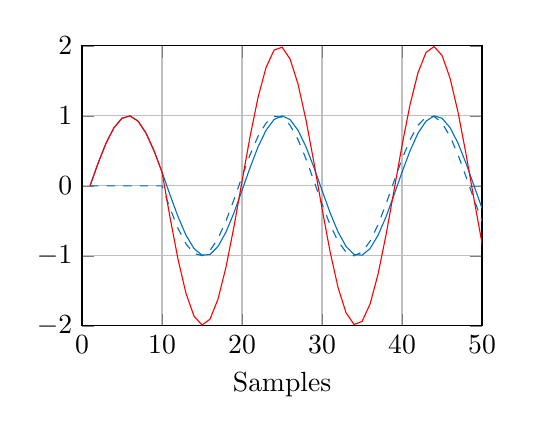
\begin{tikzpicture}

\begin{axis}[%
width=2in,
height=1.4in,
xlabel = {Samples},
%ylabel = {Amplitude}, 
scale only axis,
xmin=0,
xmax=50,
xmajorgrids,
ymin=-2,
ymax=2,
ymajorgrids,
axis background/.style={fill=white}
]
\addplot [color=mycolor1,solid,forget plot]
  table[row sep=crcr]{%
1	0\\
2	0.321439465303162\\
3	0.608761429008721\\
4	0.831469612302545\\
5	0.965925826289068\\
6	0.997858923238603\\
7	0.923879532511287\\
8	0.751839807478978\\
9	0.5\\
10	0.195090322016128\\
11	-0.130526192220051\\
12	-0.442288690219001\\
13	-0.707106781186548\\
14	-0.896872741532688\\
15	-0.99144486137381\\
16	-0.98078528040323\\
17	-0.866025403784439\\
18	-0.659345815100069\\
19	-0.38268343236509\\
20	-0.0654031292301428\\
21	0.25881904510252\\
22	0.555570233019602\\
23	0.793353340291235\\
24	0.946930129495105\\
25	1\\
26	0.946930129495106\\
27	0.793353340291235\\
28	0.555570233019604\\
29	0.258819045102523\\
30	-0.0654031292301431\\
31	-0.38268343236509\\
32	-0.659345815100069\\
33	-0.866025403784438\\
34	-0.98078528040323\\
35	-0.991444861373811\\
36	-0.896872741532689\\
37	-0.707106781186547\\
38	-0.442288690219002\\
39	-0.130526192220051\\
40	0.195090322016127\\
41	0.499999999999999\\
42	0.751839807478976\\
43	0.923879532511286\\
44	0.997858923238604\\
45	0.965925826289069\\
46	0.831469612302546\\
47	0.608761429008723\\
48	0.321439465303162\\
49	-1.16403343982657e-15\\
50	-0.321439465303164\\
51	-0.608761429008723\\
52	-0.831469612302545\\
53	-0.965925826289068\\
54	-0.997858923238603\\
55	-0.923879532511286\\
56	-0.751839807478978\\
57	-0.5\\
58	-0.195090322016128\\
59	0.130526192220052\\
60	0.442288690218998\\
61	0.707106781186548\\
62	0.89687274153269\\
63	0.99144486137381\\
64	0.98078528040323\\
65	0.866025403784438\\
66	0.659345815100069\\
67	0.382683432365093\\
68	0.0654031292301461\\
69	-0.258819045102525\\
70	-0.555570233019603\\
71	-0.793353340291236\\
72	-0.946930129495106\\
73	-1\\
74	-0.946930129495105\\
75	-0.793353340291237\\
76	-0.555570233019604\\
77	-0.25881904510252\\
78	0.0654031292301442\\
79	0.382683432365091\\
80	0.65934581510007\\
81	0.866025403784439\\
82	0.98078528040323\\
83	0.991444861373811\\
84	0.896872741532689\\
85	0.707106781186549\\
86	0.442288690219003\\
87	0.13052619222005\\
88	-0.19509032201613\\
89	-0.499999999999999\\
90	-0.751839807478979\\
91	-0.923879532511286\\
92	-0.997858923238603\\
93	-0.965925826289069\\
94	-0.831469612302548\\
95	-0.608761429008722\\
96	-0.321439465303163\\
97	2.32806687965315e-15\\
};
\addplot [color=mycolor1,dashed,forget plot]
  table[row sep=crcr]{%
1	0\\
2	0\\
3	0\\
4	0\\
5	0\\
6	0\\
7	0\\
8	0\\
9	0\\
10	0\\
11	-0.321439465303162\\
12	-0.608761429008721\\
13	-0.831469612302545\\
14	-0.965925826289068\\
15	-0.997858923238603\\
16	-0.923879532511287\\
17	-0.751839807478978\\
18	-0.5\\
19	-0.195090322016128\\
20	0.130526192220051\\
21	0.442288690219001\\
22	0.707106781186548\\
23	0.896872741532688\\
24	0.99144486137381\\
25	0.98078528040323\\
26	0.866025403784439\\
27	0.659345815100069\\
28	0.38268343236509\\
29	0.0654031292301428\\
30	-0.25881904510252\\
31	-0.555570233019602\\
32	-0.793353340291235\\
33	-0.946930129495105\\
34	-1\\
35	-0.946930129495106\\
36	-0.793353340291235\\
37	-0.555570233019604\\
38	-0.258819045102523\\
39	0.0654031292301431\\
40	0.38268343236509\\
41	0.659345815100069\\
42	0.866025403784438\\
43	0.98078528040323\\
44	0.991444861373811\\
45	0.896872741532689\\
46	0.707106781186547\\
47	0.442288690219002\\
48	0.130526192220051\\
49	-0.195090322016127\\
50	-0.499999999999999\\
51	-0.751839807478976\\
52	-0.923879532511286\\
53	-0.997858923238604\\
54	-0.965925826289069\\
55	-0.831469612302546\\
56	-0.608761429008723\\
57	-0.321439465303162\\
58	1.16403343982657e-15\\
59	0.321439465303164\\
60	0.608761429008723\\
61	0.831469612302545\\
62	0.965925826289068\\
63	0.997858923238603\\
64	0.923879532511286\\
65	0.751839807478978\\
66	0.5\\
67	0.195090322016128\\
68	-0.130526192220052\\
69	-0.442288690218998\\
70	-0.707106781186548\\
71	-0.89687274153269\\
72	-0.99144486137381\\
73	-0.98078528040323\\
74	-0.866025403784438\\
75	-0.659345815100069\\
76	-0.382683432365093\\
77	-0.0654031292301461\\
78	0.258819045102525\\
79	0.555570233019603\\
80	0.793353340291236\\
81	0.946930129495106\\
82	1\\
83	0.946930129495105\\
84	0.793353340291237\\
85	0.555570233019604\\
86	0.25881904510252\\
87	-0.0654031292301442\\
88	-0.382683432365091\\
89	-0.65934581510007\\
90	-0.866025403784439\\
91	-0.98078528040323\\
92	-0.991444861373811\\
93	-0.896872741532689\\
94	-0.707106781186549\\
95	-0.442288690219003\\
96	-0.13052619222005\\
97	0.19509032201613\\
98	0.499999999999999\\
99	0.751839807478979\\
100	0.923879532511286\\
101	0.997858923238603\\
102	0.965925826289069\\
103	0.831469612302548\\
104	0.608761429008722\\
105	0.321439465303163\\
106	-2.32806687965315e-15\\
};
\addplot [color=red,solid,forget plot]
  table[row sep=crcr]{%
1	0\\
2	0.321439465303162\\
3	0.608761429008721\\
4	0.831469612302545\\
5	0.965925826289068\\
6	0.997858923238603\\
7	0.923879532511287\\
8	0.751839807478978\\
9	0.5\\
10	0.195090322016128\\
11	-0.451965657523213\\
12	-1.05105011922772\\
13	-1.53857639348909\\
14	-1.86279856782176\\
15	-1.98930378461241\\
16	-1.90466481291452\\
17	-1.61786521126342\\
18	-1.15934581510007\\
19	-0.577773754381218\\
20	0.0651230629899085\\
21	0.701107735321521\\
22	1.26267701420615\\
23	1.69022608182392\\
24	1.93837499086892\\
25	1.98078528040323\\
26	1.81295553327954\\
27	1.4526991553913\\
28	0.938253665384693\\
29	0.324222174332665\\
30	-0.324222174332663\\
31	-0.938253665384692\\
32	-1.4526991553913\\
33	-1.81295553327954\\
34	-1.98078528040323\\
35	-1.93837499086892\\
36	-1.69022608182392\\
37	-1.26267701420615\\
38	-0.701107735321525\\
39	-0.065123062989908\\
40	0.577773754381217\\
41	1.15934581510007\\
42	1.61786521126341\\
43	1.90466481291452\\
44	1.98930378461241\\
45	1.86279856782176\\
46	1.53857639348909\\
47	1.05105011922773\\
48	0.451965657523213\\
49	-0.195090322016128\\
50	-0.821439465303163\\
51	-1.3606012364877\\
52	-1.75534914481383\\
53	-1.96378474952767\\
54	-1.96378474952767\\
55	-1.75534914481383\\
56	-1.3606012364877\\
57	-0.821439465303162\\
58	-0.195090322016127\\
59	0.451965657523216\\
60	1.05105011922772\\
61	1.53857639348909\\
62	1.86279856782176\\
63	1.98930378461241\\
64	1.90466481291452\\
65	1.61786521126342\\
66	1.15934581510007\\
67	0.577773754381221\\
68	-0.0651230629899055\\
69	-0.701107735321523\\
70	-1.26267701420615\\
71	-1.69022608182393\\
72	-1.93837499086892\\
73	-1.98078528040323\\
74	-1.81295553327954\\
75	-1.45269915539131\\
76	-0.938253665384697\\
77	-0.324222174332666\\
78	0.324222174332669\\
79	0.938253665384694\\
80	1.45269915539131\\
81	1.81295553327955\\
82	1.98078528040323\\
83	1.93837499086892\\
84	1.69022608182393\\
85	1.26267701420615\\
86	0.701107735321523\\
87	0.0651230629899057\\
88	-0.577773754381221\\
89	-1.15934581510007\\
90	-1.61786521126342\\
91	-1.90466481291452\\
92	-1.98930378461241\\
93	-1.86279856782176\\
94	-1.5385763934891\\
95	-1.05105011922772\\
96	-0.451965657523213\\
97	0.195090322016132\\
};
\end{axis}
\end{tikzpicture}%
	 		%\caption{2500 Hz}
	 	\end{center}
		\end{column}
	\end{columns}
\end{frame}

\begin{frame}{Influence of system delay}{Problem of ANC}		
	\begin{center}
	\begin{itemize}
	\item System delay determine the frequency range that can be attenuated
	\item Low frequency are well attenuated by active systems
	\item High frequencies are passively damped by the headphone cup 
	\end{itemize}
	\end{center}
\end{frame}


\begin{frame}{Present Consumer Headphones}{Performance}
	\begin{itemize}	
	\item How well does the consumer headphones ANC attenuate?
	\begin{columns}
		\begin{column}{0.27\textwidth}
		\begin{itemize}
			\item Denon AH-GC20
			\item Bose QC25 
			\item Bose QC15 	
			\item BeoPlay H8 	
		\end{itemize}
		\end{column}
		\begin{column}{0.6\textwidth} 
		\begin{itemize}
			\item[] 2.200 kr (2016)
			\item[] 2.799 kr (2016)
			\item[] 2.696 kr (2011)
			\item[] 3.495 kr (2016)
		\end{itemize}
		\end{column}
	\end{columns}
	\end{itemize}			
	\begin{center}
		% This file was created by matlab2tikz.
%
%The latest updates can be retrieved from
%  http://www.mathworks.com/matlabcentral/fileexchange/22022-matlab2tikz-matlab2tikz
%where you can also make suggestions and rate matlab2tikz.
%
\definecolor{mycolor1}{rgb}{0.00000,0.44700,0.74100}%
\definecolor{mycolor2}{rgb}{0.85000,0.32500,0.09800}%
\definecolor{mycolor3}{rgb}{0.92900,0.69400,0.12500}%
\definecolor{mycolor4}{rgb}{0.49400,0.18400,0.55600}%
%
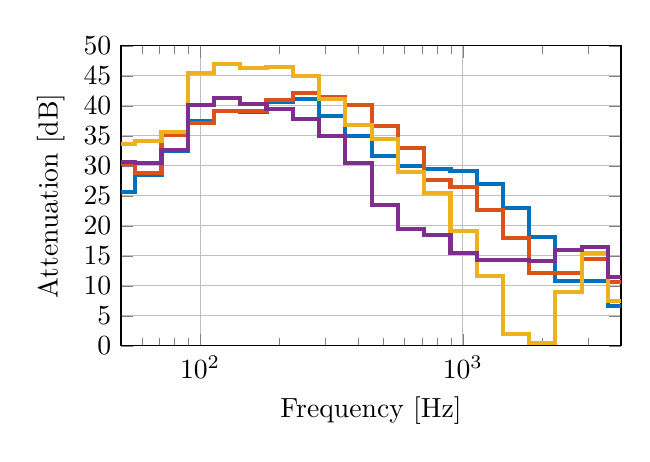
\begin{tikzpicture}

\begin{axis}[%
width=2.5in,
height=1.5in,
at={(1.011in,0.642in)},
scale only axis,
xmode=log,
xmin=50,
xmax=4000,
xlabel={Frequency [Hz]},
xmajorgrids,
%xmajorgrids,
%ymajorgrids,
%xminorgrids,
ymin=0,
ymax=50,
ytick={0,5,...,50},
ylabel={Attenuation [dB]},
ymajorgrids,
axis background/.style={fill=white},
title style={font=\bfseries},
%title={Comparison of Smoothened curves},
legend style={legend cell align=left,align=left,draw=white!15!black}
]
%\addplot[const plot,color=mycolor1,solid,forget plot,thick] plot table[row sep=crcr] {%
%	28.4	15.7\\
%	35.7	15.1\\
%	45	12.4\\
%	56.6	14\\
%	71.3	16.3\\
%	89.7	18.8\\
%	113	19.6\\
%	142	19.5\\
%	179	20.3\\
%	225	20.4\\
%	284	19.2\\
%	357	17.4\\
%	450	15.7\\
%	566	15.1\\
%	713	14.7\\
%	897	14.5\\
%	1.13e+03	13.5\\
%	1.42e+03	11.5\\
%	1.79e+03	9.08\\
%	2.25e+03	5.31\\
%	2.84e+03	5.51\\
%	3.57e+03	3.03\\
%	4.5e+03	2.37\\
%	5.66e+03	2.81\\
%	7.13e+03	3.07\\
%	8.97e+03	3.24\\
%	1.13e+04	1.16\\
%	1.42e+04	0.032\\
%	1.79e+04	0.598\\
%	2e+04	-0.763\\
%};
%\addplot[const plot,color=mycolor2,solid,forget plot,thick] plot table[row sep=crcr] {%
%	28.4	14.7\\
%	35.7	15.3\\
%	45	15.2\\
%	56.6	14.2\\
%	71.3	17.6\\
%	89.7	18.7\\
%	113	19.5\\
%	142	19.5\\
%	179	20.4\\
%	225	21.3\\
%	284	20.8\\
%	357	19.8\\
%	450	18.4\\
%	566	16.5\\
%	713	13.4\\
%	897	13.2\\
%	1.13e+03	11.4\\
%	1.42e+03	8.6\\
%	1.79e+03	6.11\\
%	2.25e+03	6.07\\
%	2.84e+03	7.27\\
%	3.57e+03	4.99\\
%	4.5e+03	2.6\\
%	5.66e+03	2.91\\
%	7.13e+03	1.03\\
%	8.97e+03	2.02\\
%	1.13e+04	-0.338\\
%	1.42e+04	-0.849\\
%	1.79e+04	-0.618\\
%	2e+04	-2.19\\
%};
%\addplot[const plot,color=mycolor3,solid,forget plot,thick] plot table[row sep=crcr] {%
%	28.4	18.1\\
%	35.7	19\\
%	45	17.1\\
%	56.6	16.5\\
%	71.3	18.6\\
%	89.7	22.8\\
%	113	23.6\\
%	142	23.3\\
%	179	23.5\\
%	225	22.6\\
%	284	20.4\\
%	357	18.4\\
%	450	17.2\\
%	566	14.5\\
%	713	12.7\\
%	897	9.48\\
%	1.13e+03	5.89\\
%	1.42e+03	1.04\\
%	1.79e+03	0.132\\
%	2.25e+03	4.45\\
%	2.84e+03	7.76\\
%	3.57e+03	3.73\\
%	4.5e+03	2.58\\
%	5.66e+03	2.46\\
%	7.13e+03	1.18\\
%	8.97e+03	1.16\\
%	1.13e+04	0.0281\\
%	1.42e+04	-0.34\\
%	1.79e+04	-0.623\\
%	2e+04	-1.08\\
%};
%\addplot[const plot,color=mycolor4,solid,forget plot,thick] plot table[row sep=crcr] {%
%	28.4	18.6\\
%	35.7	16.5\\
%	45	15.5\\
%	56.6	15.5\\
%	71.3	16.6\\
%	89.7	20.3\\
%	113	20.4\\
%	142	20\\
%	179	19.6\\
%	225	18.9\\
%	284	17.4\\
%	357	15.3\\
%	450	11.8\\
%	566	9.77\\
%	713	8.89\\
%	897	7.71\\
%	1.13e+03	6.86\\
%	1.42e+03	7.05\\
%	1.79e+03	7.37\\
%	2.25e+03	7.85\\
%	2.84e+03	8.24\\
%	3.57e+03	5.7\\
%	4.5e+03	3.78\\
%	5.66e+03	3.02\\
%	7.13e+03	1.43\\
%	8.97e+03	1.33\\
%	1.13e+04	1.58\\
%	1.42e+04	0.0462\\
%	1.79e+04	-1.02\\
%	2e+04	-0.621\\
%};
%\end{axis}

%% 20 log
\addplot[const plot,color=mycolor1,solid,line width=1.5pt,forget plot] plot table[row sep=crcr] {%
	28.4	30.6\\
	35.7	31.3\\
	45	25.7\\
	56.6	28.5\\
	71.3	32.4\\
	89.7	37.4\\
	113	39.1\\
	142	39\\
	179	40.6\\
	225	41.2\\
	284	38.3\\
	357	35\\
	450	31.7\\
	566	30\\
	713	29.4\\
	897	29.1\\
	1.13e+03	27\\
	1.42e+03	23\\
	1.79e+03	18.2\\
	2.25e+03	10.8\\
	2.84e+03	10.8\\
	3.57e+03	6.62\\
	4.5e+03	4.92\\
	5.66e+03	5.21\\
	7.13e+03	5.95\\
	8.97e+03	5.98\\
	1.13e+04	2.27\\
	1.42e+04	-1\\
	1.79e+04	0.842\\
	2e+04	-1.38\\
};
\addplot[const plot,color=mycolor2,solid,line width=1.5pt,forget plot] plot table[row sep=crcr] {%
	28.4	29.3\\
	35.7	30.1\\
	45	30.3\\
	56.6	28.8\\
	71.3	35.2\\
	89.7	37.2\\
	113	39.1\\
	142	39.2\\
	179	41\\
	225	42.2\\
	284	41.5\\
	357	40.1\\
	450	36.7\\
	566	33\\
	713	27.7\\
	897	26.5\\
	1.13e+03	22.7\\
	1.42e+03	17.9\\
	1.79e+03	12.1\\
	2.25e+03	12.1\\
	2.84e+03	14.4\\
	3.57e+03	10.6\\
	4.5e+03	5.72\\
	5.66e+03	5.17\\
	7.13e+03	2.13\\
	8.97e+03	4.17\\
	1.13e+04	-0.138\\
	1.42e+04	-0.907\\
	1.79e+04	-1.96\\
	2e+04	-4.33\\
};
\addplot[const plot,color=mycolor3,solid,line width=1.5pt,forget plot] plot table[row sep=crcr] {%
	28.4	36.2\\
	35.7	38.5\\
	45	33.6\\
	56.6	34.2\\
	71.3	35.6\\
	89.7	45.5\\
	113	46.9\\
	142	46.3\\
	179	46.5\\
	225	44.9\\
	284	41.1\\
	357	36.8\\
	450	34.5\\
	566	29\\
	713	25.5\\
	897	19.1\\
	1.13e+03	11.6\\
	1.42e+03	1.91\\
	1.79e+03	0.429\\
	2.25e+03	9.03\\
	2.84e+03	15.5\\
	3.57e+03	7.47\\
	4.5e+03	4.95\\
	5.66e+03	4.31\\
	7.13e+03	2.18\\
	8.97e+03	2.87\\
	1.13e+04	0.264\\
	1.42e+04	-0.554\\
	1.79e+04	-2.08\\
	2e+04	-2.36\\
};
\addplot[const plot,color=mycolor4,solid,line width=1.5pt,forget plot] plot table[row sep=crcr] {%
	28.4	37.2\\
	35.7	33.9\\
	45	30.7\\
	56.6	30.4\\
	71.3	32.7\\
	89.7	40.2\\
	113	41.3\\
	142	40.3\\
	179	39.5\\
	225	37.8\\
	284	34.9\\
	357	30.5\\
	450	23.4\\
	566	19.5\\
	713	18.4\\
	897	15.4\\
	1.13e+03	14.3\\
	1.42e+03	14.3\\
	1.79e+03	14.1\\
	2.25e+03	16\\
	2.84e+03	16.4\\
	3.57e+03	11.5\\
	4.5e+03	7.26\\
	5.66e+03	6.34\\
	7.13e+03	2.99\\
	8.97e+03	2.87\\
	1.13e+04	2.9\\
	1.42e+04	0.784\\
	1.79e+04	-1.51\\
	2e+04	-1.74\\
};
\end{axis}
\end{tikzpicture}%
	\end{center}	
\end{frame}

\subsection{Strategy}
\begin{frame}{Strategy}
	\begin{center}
	\begin{itemize}
		\item Improve the frequency range of the attenuation
		\item Reducing system delay
		\begin{itemize}	
		\item Multirate processing
		\item Linear prediction
		\end{itemize}				
	\end{itemize}
	\end{center}
\end{frame}

\begin{frame}{Prediction and feedforward system overview}
	\begin{center}
		\resizebox{1\columnwidth}{!}{
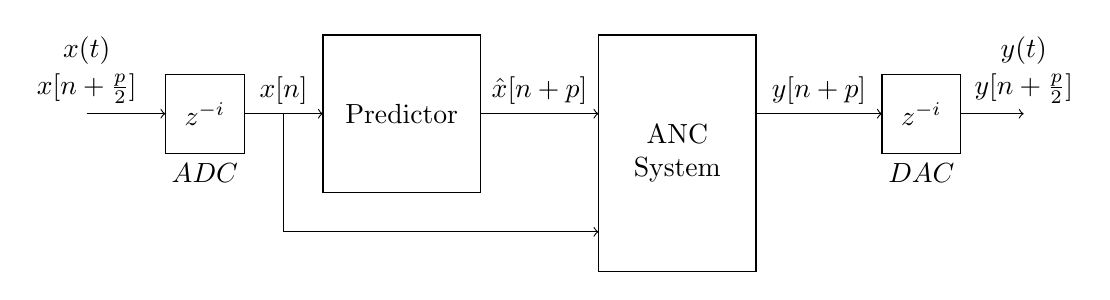
\begin{tikzpicture}
\draw  (-4,1.5) rectangle node {$z^{-i}$} (-5,0.5);
\draw (-4.5,0) node[above]{$ADC$} ;

\draw  (-3,2) rectangle  node[align=center] {Predictor} (-1,0) ;

\draw  (0.5,2) rectangle node[text width=1.5cm,align=center] {ANC System}(2.5,-1);
\draw  (4.1,1.5) rectangle node {$z^{-i}$}(5.1,0.5);
\draw (4.6,0) node[above]{$DAC$} ;

\draw [->](-4,1)  -- (-3,1);


\draw [->](-1,1)  -- node[above]{$\hat{x}[n+p]$}  (0.5,1);
\draw [->](2.5,1) -- node[above]{$y[n+p]$} (4.1,1);

\draw [->](-6,1) node[above]{$x[n+\frac{p}{2}]$} -- (-5,1);
\draw (-6,1.5) node[above]{$x(t)$} ;
\draw [->](5.1,1)-- (5.9,1) node[above]{$y[n+\frac{p}{2}]$} ;
\draw [->](-3.5,1) node[above]{$x[n]$} -- (-3.5,-0.5) -- (0.5,-0.5);
\draw (5.9,1.5) node[above]{$y(t)$} ;
\end{tikzpicture}}	
	\end{center}
\end{frame}
